% ****** Start of file apssamp.tex ******
%
%   This file is part of the APS files in the REVTeX 4 distribution.
%   Version 4.0 of REVTeX, August 2001
%
%   Copyright (c) 2001 The American Physical Society.
%
%   See the REVTeX 4 README file for restrictions and more information.
%
% TeX'ing this file requires that you have AMS-LaTeX 2.0 installed
% as well as the rest of the prerequisites for REVTeX 4.0
%
% See the REVTeX 4 README file
% It also requires running BibTeX. The commands are as follows:
%
%  1)  latex apssamp.tex
%  2)  bibtex apssamp
%  3)  latex apssamp.tex
%  4)  latex apssamp.tex
%
\documentclass[twocolumn,amsmath,amssymb,10pt,groupedaddress,a4paper]{revtex4}
%\documentclass[preprint,showpacs,preprintnumbers,amsmath,amssymb]{revtex4}

% Some other (several out of many) possibilities
%\documentclass[preprint,aps]{revtex4}
%\documentclass[preprint,aps,draft]{revtex4}
%\documentclass[prb]{revtex4}% Physical Review B
%\documentclass[preprint,aps]{revtex4}
%\documentclass[preprint,eqsecnum,aps]{revtex4}
%\documentclass[eqsecnum,aps]{revtex4}
%\tightenlines
%\usepackage[dvips]{graphicx}
%\usepackage{amssymb}
%\usepackage{floatflt}
%\usepackage{array}

%\begin{document}

\usepackage{graphicx}% Include figure files
\usepackage{dcolumn}% Align table columns on decimal point
\usepackage{bm}% bold math
%\usepackage{array}
\usepackage{fancyheadings}
\pagestyle{fancy}
%\usepackage{longtable}
% \usepackage{multirow}
\usepackage[active]{srcltx}
%\usepackage{bibunits}% Separate lists of references
%\usepackage[bookmarksnumbered,colorlinks,backref, bookmarks, breaklinks, linktocpage]{hyperref}
\bibliographystyle{ieeetr.bst}

%\setlongtables
%\nofiles

\begin{document}

\preprint{Nuclear Data Sheets}
%\draft
\title{EMPIRE: Integrated Nuclear Theory System for  Evaluation of Nuclear Reactions }


\author{M. Herman}
\affiliation{National Nuclear Data Center, Brookhaven National Laboratory, Upton~NY~11973-5000}
\author{R. Capote}
\affiliation{Nuclear Data Section, International Atomic Energy Agency, Vienna, Austria}
\author{B. Carlson}
\affiliation{ITA/Centro Tecnico Aeroespacial, Sao Jose dos Campos, Brazil}
\author{P. Oblo\v zinsk\'y}
\affiliation{National Nuclear Data Center, Brookhaven National Laboratory, Upton~NY~11973-5000. }
\author{M. Sin}
\affiliation{Nuclear Physics Department, Bucharest University, Bucharest-Magurele, Romania}
\author{A. Trkov }
\affiliation{Jozef Stefan Institute, Ljubljana, Slovenia}
% \author{S. F. Mughabghab}
% \affiliation{National Nuclear Data Center, Brookhaven National Laboratory, Upton~NY~11973-5000 }
\author{H. Wienke}
\affiliation{Belgonucleaire, B2480, Dessel, Belgium}
\author{V. Zerkin}
\affiliation{Nuclear Data Section, International Atomic Energy Agency, Vienna, Austria }
%\author{T. Kawano}
%\affiliation{T-16, Los Alamos National Laboratory, Los Alamos, NM 87545}
% \author{Young-Sik Cho}
% \affiliation{Korea Atomic Energy Research Institute, Nuclear Data Evaluation Lab., Daejeon, Korea}
% \author{D. Rochman}
% \affiliation{National Nuclear Data Center, Brookhaven National Laboratory, Upton~NY~11973-5000- }

\begin{abstract}

EMPIRE is a modular system of nuclear reaction codes, comprising various
nuclear models, and designed for calculations over a broad range of
energies and incident particles. A projectile can be neutron, proton, any ion
(including Heavy Ions) or a photon. The energy range extends up to few hundred
MeV for Heavy Ion induced reactions while for neutron reactions it covers also
the resonance region through a module accessing Atlas of Neutron Resonances.
The code accounts for the major
nuclear reaction mechanisms, such as optical model, Coupled Channels
and DWBA (ECIS03), deformation dependent Multi-step Direct (ORION + TRISTAN), NVWY Multi-step
Compound, exciton model with cluster emission (PCROSS)  and another one
with full angular momentum coupling (DEGAS) and the full featured Hauser-Feshbach
model with $\gamma$-cascade and widths fluctuations. Advanced treatment of the
fission channel takes into account transmission through a triple humped fission
barrier with absorption in the wells. The fission probability is derived in WKB
approximation within optical model for fission. This formalism is capable of describing the
complex resonant structure in the neutron induced fission on light actinides.
Several options for level
densities include EMPIRE-specific approach accounting for effects of the dynamic deformation
of a fast rotating nucleus, the classical Gilbert-Cameron, and the tables precalculated with
a microscopic model.
Heavy Ion fusion cross section can be calculated within the
simplified coupled channels approach (CCFUS). A comprehensive library
of input parameters covers nuclear masses, optical model parameters,
ground state deformations, discrete levels and decay schemes, level
densities, fission barriers, moments of inertia (MOMFIT),
and $\gamma$-ray strength functions.
The results can be converted into the ENDF-6 format using the accompanying
code EMPEND and completed with neutron resonances extracted from the existing evaluations.
Capabilities of generating covariances, using both KALAMN and Monte Carlo methods,
are the most recent extensions of the system and are still being advanced and refined.
The package contains the full EXFOR
library of experimental data that are automatically retrieved during the
calculations. Publication quality graphs can be obtained using the powerful
and flexible plotting package ZVView. The graphic user interface, written
in Tcl/Tk, provides for easy operation of the system. This paper describes
capabilities of the code, outlines physical models and indicates parameter libraries
used for theory based predictions of cross sections and spectra provided by EMPIRE.

\end{abstract}

\maketitle
\lhead{Nuclear Reaction Evaluation...}
\chead{NUCLEAR DATA SHEETS}
\rhead{M. Herman \textit{et al.}}
\lfoot{}
\rfoot{}
\setlength{\headrulewidth}{0.4pt}
\setlength{\footrulewidth}{0.4pt}

\newpage
\tableofcontents



\newpage
%%%%%%%%%%%%%%%%%%%%%%%%%%%%%%%%%%%%%%%%%%%%%%%%%%%%%%%%%%%%%%%%%%%%%%%%%%%%%%%%%%%%%%%%%%%%%%%%%%%%%%%%%%%%%%%%%%
\section{ToDo and deficiencies}

\begin{itemize}
\item CC and DWBA should be updated
\item Fission should be updated
\item GUI to be included
\item OMP fitting to be included
\item PCROSS to be expanded
\item gamma-strength functions to be expanded with the new ones
\item Plots to be improved
\item Covariances to be written
\item Formatting updated with isomeric cross sections and mixed exclusive/inclusive spectra
\end{itemize}

\section{Overview of the EMPIRE-2 system}

The origin of the EMPIRE-2 system can be traced back to the statistical model
code EMPIRE~\cite{EMPIRE-I} coded by M. Herman and first released in 1980.
This initial version had been extended over following years by adding modern
approaches to preequilibrium emission such as FKK~\cite{FKK} and NVWY~\cite{NVWY}
formulations of the Multi-step Compound mechanism, and combinatorial
calculations of particle-hole level densities. In addition, a version for
Heavy Ion induced reactions (EMPIRE HI) was developed.

EMPIRE-2 is a totally new development although it benefits from the experience
gained with the previous version. The present code
has been rewritten from scratch, using more advanced programming concepts.
It has been designed to be general and flexible, and can been applied
to the calculation of neutron capture in the keV region, as well as
to Heavy Ion (HI) induced reactions at several hundreds of MeV. The aim is to
provide a powerful environment for modeling nuclear reactions that can be used
in basic research as well as for generation of the evaluated nuclear data files.
To achieve this goal we implement in a single system an extensive set of
models that cover all most important nuclear reaction mechanisms up to the
threshold for pion production. At the same time we also provide a complete set of reaction channels and
observables that might be of interest to nuclear applications. These observables include
cross sections, spectra, angular distributions and angle-energy correlated spectra
(double-differential cross sections) for nucleons, $\alpha$-particles, light ions
and $\gamma$-rays, as well as cross sections for population of isomeric levels
(activation cross sections). Such extensive calculations require a considerable amount
of input parameters. To provide them EMPIRE incorporates a comprehensive library of model
parameters, largely based on the IAEA RIPL-2~\cite{RIPL-2} project
although the preliminary recommendations of the follow up edition (RIPL-3) are used when available. The calculated results
can be plotted and compared against available experimental data automatically extracted
from the EXFOR library~\cite{EXFOR}.

The large part of the EMPIRE-2 system is dedicated to the
particular exigencies encountered in nuclear data evaluation. These include ENDF-6 formatting
of the calculated results, verification of the file, its preprocessing, plotting and the ultimate check consisting in processing the file with the NJOY code. Due to the high level of
integration between various components of EMPIRE-2, and intuitive control ensured by the
User Graphic Interface (GUI) the operation of the whole system is very easy.  Most intermediate steps
are transparent to the user.  In an extreme case of accepting all defaults, a complete ENDF-6 formatted file, including graphical comparison with experimental data and full verification with the checking
codes can be created just by typing in atomic and mass numbers for the target followed by a couple of mouse-clicks.

The flowchart of the EMPIRE-2 system is shown in Fig.~\ref{Fig:empire-flowchart}.
The entire EMPIRE-2 system can be divided into four major components:
\begin{enumerate}
\item physics core,
\item input parameter library,
\item scripts and GUIs,
\item utility codes,
\item experimental data library (EXFOR).
\end{enumerate}
The physics core, supported by the input parameter library, is a heart of the system. It consists of a number of modules that implement various nuclear reaction theory models. The selection of these models is very pragmatical - we try to cover all important features of nuclear reactions using modern, physically sound theoretical approaches  that are computationally reasonable.  Accordingly,
we employ DWBA and Coupled-Channels methods to be able to deal with deformed nuclei, classical and quantum-mechanical preequilibrium models to account for precompound effects at higher incident energies, and a sophisticated approach to fission in order to describe structure in the fission cross section on minor actinides. The major part of the incoming flux is treated in terms of the Hauser-Feshbach formalism with account for width fluctuation effects. On the other hand, we put aside certain highly advanced formulations that would result in prohibitively lengthy or complex calculations (e.g., the triple-integral approach to width fluctuations, microscopic calculations of input quantities, exact treatment of the compound nucleus reactions in presence of strong direct channels, etc.). These respectful advances will hopefully become part of the EMPIRE in future but their inclusion in the current version would compromise practical usefulness of the code for a general user. Nevertheless, certain input parameters obtained using microscopic theories  are tabulated and made available to EMPIRE-2 through the RIPL library.

The physics core of EMPIRE is a mixture of the original coding and of several codes, written by different authors, which
were converted into subroutines and adapted for the present use.
In most cases, the modifications concerned input/output interface
and never affected the physical model contained in the original source.
The following codes are incorporated in the core of the EMPIRE:
\begin{description}
\item [\textbf{ECIS03\index{ECIS}}]Coupled-Channels\index{Coupled-Channels}
and DWBA\index{DWBA} code by J. Raynal~\cite{ECIS},
\item [\textbf{CCFUS\index{CCFUS}}]simplified Coupled-Channels calculation
of HI fusion cross section by C.H. Dasso and S. Landowne~\cite{CCFUS},
\item [\textbf{ORION\index{ORION}~\&~TRISTAN\index{TRISTAN}}]TUL\index{TUL}~\cite{TUL}
approach to Multi-step Direct\index{MSD} by H. Lenske~\cite{ORTRI},
\item [\textbf{DEGAS\index{DEGAS}}]exciton model with angular momentum
conservation and $\gamma$ emission~\cite{Degas} by E. B\v et\' ak
and P. Oblo\v zinsk\' y,
\item [\textbf{DDHMS\index{DDHMS}}]Monte Carlo simulation of the preequilibrium
decay by M.B. Chadwick~\cite{DDHMScode}
\item [\textbf{BARMOM\index{BARMOM}}]fission barriers and moments of inertia
by A. Sierk~\cite{sierk}.
\end{description}
The reader is referred to the original papers for a more detailed
description of these incorporated codes. Furthermore, the package
includes a number of stand-alone utility codes that are listed in Sec.~\ref{Sec:utility-codes}


Completeness and ease of use have always been the two functional aspects that guided development of the EMPIRE system.
The utility codes, scripts and GUI's are instrumental in making EMPIRE user friendly. Regrding the other aspect, we strive to provide ultimately all functionalities necessary or useful for nuclear data evaluation. The three recent extensions bring us closer to this goal: (i) the highly automated module for adjustment of optical potential parameters, (ii) the resonance module bringing capability of extracting, analyzing and formating resonance parameters from the Atlas of Neutron Resonances~\cite{Mughabghab:06}, and (iii) the covariance module enabling quantification of nuclear data uncertainties using both Monte Carlo and Kalman methods to combine experimental covariances with the model based ones. The latter two extensions, although well advanced, are still in a phase of development and testing. Therefore, we will not cover them extensively in the present paper

We are pleased to acknowledge existence of similar all-in-one codes that built on a comparable physics, use alike design concepts, aim at analogous targets and address akin users. In the first place we mention the TALYS code~\cite{TALYS}, the original development by the Dutch-French collaboration, and the McGANSH code - being developed at Los Alamos as the successor to the well known and widely used GNASH code. We are also aware of the two independent activities carried out at JAEA in Japan. This healthy and friendly competition is a sign of vigorousness of the field and should bring considerable benefits. The codes differ in the selection of the reaction models, tend to employ somewhat different implementations, and provide unique  features that make them better tailored to particular problems. The comparison of calculated results provides insight into accuracies of the models, approximations involved in their implementation and, last but not least, it helps to discover and correct coding errors that otherwise would be difficult to detect ("errare humanum est perseverare diabolicum" Lucius Annaeus Seneca, ca. 4 BC $-$ AD 65).

In the following sections we outline physics built into various modules of the EMPIRE, contents of the input libraries and particular features offered by the code. The intention of this writeup is to present capabilities of the EMPIRE system and explain means it is using to produce the answer. Even with the relatively generous space available to this review it is not possible to document all minor features and details of the algorithms used in the code. In particular, input preparation and operation of the code are outside the scope of the present paper. Users are advised to consult EMPIRE manual available at www.nndc.bnl.gov/empire and www-nds.iaea.org/empire for more practical instructions. Similarly, we
refer to the Ref.~\cite{Mughabghab:06} for details concerning evaluation of neutron resonances and to RIPL-2 documentation~\cite{RIPL-2} for particulars regarding input parameter library.

\section{Physics core of EMPIRE-2}

%%%%%%%%%%%%%%%%%%%%%%%%%%%%%%%%%%%%%%%%%%%%%%%%%%%%%%%%%%%%%%%%%%%%%%%%%%%%%%%%%%%%%%%%%%%%%%%%%%%%%%%%%%%%%%%%%%
\subsection{Fusion, Optical Model and Direct Reactions}
%%%%%%%%%%%%%%%%%%%%%%%%%%%%%%%%%%%%%%%%%%%%%%%%%%%%%%%%%%%%%%%%%%%%%%%%%%%%%%%%%%%%%%%%%%%%%%%%%%%%%%%%%%%%%%%%%%
\subsubsection{Fusion/reaction cross section\label{sec: fusion}}
The reaction cross section is calculated in terms of transmission
coefficients $T_{l}^{a}(\epsilon)$ using the expression

\begin{eqnarray}
\sigma_{a}(U,J,\pi)&=&\frac{\pi}{k^{2}}\frac{(2J+1)}{(2I+1)(2i+1)}\sum_{S=|I-i|}^{I+i}\sum_{l=|J-S|}^{J+S}\nonumber\\
                   & &f(l,\pi)T_{l}^{a}(\epsilon),
\label{fusion}
\end{eqnarray}

\noindent where $k$ is the wave number of relative motion, $i,I,J,$
and $S$ indicate projectile, target, compound nucleus, and channel
spin, respectively, and $l$ is the orbital angular momentum of the
projectile $a$. The function $f(l,\pi)$ ensures parity conservation.
It is unity if $p*P*(-1)^{l}=\pi$ and zero otherwise. Here $p,\, P,$
and $\pi$ are projectile, target, and compound nucleus parities and
$\epsilon$ and $U$ stand for the projectile and compound nucleus
energy. The way the transmission coefficients entering Eq.~\ref{fusion}
are determined depends on the projectile. For those with mass numbers
A$\leq$4 transmission coefficients are traditionally determined in the frame of
spherical or deformed optical model (see Sec.~\ref{sec:DWBA-CC})
while different approaches are needed for Heavy Ions (HI) and photons.

The model for photoabsorption must account for the different reaction
mechanisms involved in the initial photonuclear excitation process
and can not be decoupled from the
subsequent decay of the excited nucleus by particle and $\gamma$-ray
emission. At low energies, below about 30 MeV, the Giant Dipole Resonance
(GDR) is the dominant excitation mechanism, while at higher
energies photoabsorption on a neutron-proton
pair (a quasi-deuteron, QD) is the dominant mechanism. Since photonuclear
reactions are described in terms of the preequilibrium models we discuss
them in more details in the Sec.~\ref{sec:photonuclear}

The Heavy Ion fusion cross section is calculated using Eq. \ref{fusion}
with transmission coefficients determined according to one of the
following methods:
\begin{itemize}
\item the simplified Coupled-Channels
approach~\cite{CCFUS} (CCFUS). Inelastic excitations
and transfer reaction channels are treated as independent modes which
couple to the initial ground state. The corresponding wave equations
are approximately uncoupled by diagonalizing the interaction at the
barrier. The total transmission probability is then obtained by summing
over the distribution of transmission probabilities for the eigenbarriers,
with weights given by the overlap of the initial state with the eigenchannels.
This is a default option. It takes into account coupling of the excited
collective states in the target and projectile. A detailed description
of the method can be found in the original reference \cite{CCFUS}.

\item the distributed fusion-barrier\index{distributed fusion-barrier}
model \cite{difusb}. This method accounts for the effective lowering
of the one-dimensional fusion barrier by allowing for the additional
dimension and assuming that the barrier distribution in the added
dimension can be represented by a truncated Gaussian. Thus the fusion
barrier distribution $f(B')$ can be characterized by the mean energy
$B$, the standard deviation $\sigma_{B}$, and the truncation parameter
$t$, and is written as
\begin{equation}
f(B')=n_{0}\exp\left(\frac{B-B'}{2\sigma_{B}^{2}}\right)^{2} \label{distbarr}
\end{equation}
\noindent for $\left|B-B'\right|<t\sigma_{B}$ and $f(B')=0$ otherwise. The
parameter $t$ defines the lowest possible value of the fusion barrier
and $n_{0}$ is the normalization factor ensuring that the integral
of Eq.~\ref{distbarr} is 1. The fusion probability for a given angular
momentum $l$ is given by a convolution of the barrier distribution
$f(B')$ and the transmission coefficient $T_{l}(E-B')$
\begin{equation}
p(E,l)=\int_{-\infty}^{\infty}f(B')T_{l}(E-B')dB'\,.
\end{equation}
\noindent The transmission coefficient in the Hill-Wheeler
approach \cite{HillWheeler} reads
\begin{equation}
T_{l}(E-B')=\left\{ 1+\exp\left[-2\pi(E-B'-E_{rot})/(\hbar\omega)\right]\right\} ^{-1}\,,
\end{equation}
\noindent with $E_{rot}$ being rotation energy at angular momentum $l$. The
distributed fusion-barrier option
in EMPIRE allows for the extra-push energy that can be specified in
the input and added to the fusion barrier. The latter, if not specified
in the input, is by default calculated using BAR subroutine of CCFUS
(see above).

\item the fusion cross sections for each $l$ read from the external
file. The code converts them into transmission
coefficients to be used in Eq.~\ref{fusion}. \\
\item the critical angular momentum $l_{cr}$ for compound nucleus
formation specified in input.
\end{itemize}

In the latter two cases the transmission coefficients are assumed
to be of the form

\begin{equation}
T_{l}^{a}(\epsilon)=\frac{1}{1+exp(-\frac{l_{cr}-l}{\delta l})}\,,\label{Tlfus}
\end{equation}

\noindent where $\delta l$ is an input parameter. If the total fusion
cross section is specified in the input, then the code adjusts $l_{cr}$
in order to reproduce the requested value.


\subsubsection{Distorted Wave Born Approximation and Coupled-Channels \label{sec:DWBA-CC}}
ECIS \cite{ECIS} is a well known and highly respected code for calculations
within the generalized optical model and Coupled-Channels model (CC).
These are important for modeling reactions on deformed nuclei and,
in particular, for the correct description of a strong population
of collective discrete levels in the inelastic scattering.  Symmetric
rotational, vibrational-rotational and harmonic-vibrational CC modes
are available. The implementation features automatic preparation of
the ECIS03 input. It uses the RIPL\index{RIPL}-2 \cite{RIPL2} optical
model segment and resorts to the RIPL-2 discrete level schemes and
to the RIPL-2 deformation parameters (quadrupole deformations
$\beta _{2}$) only if these are not included in the optical model
parameter set available from RIPL-2. The
vibrational (dynamical) deformations are defined
 as 0.15 for quadrupole and 0.05 for octupole vibrations.
Calculations can be performed for the majority of deformed nuclei
including rotational and vibrational, even-even and even-A with integer
spins, as well as odd-A with half-integer spins. Vibrational even-even
nuclei and even-A are also covered.

As an example, angular distribution for the neutron elastic scattering on $^{157}$Gd
is presented in Fig.~\ref{njoygd157}.
\begin{figure}[htbp]
\scalebox{0.17}{\includegraphics{njoygd15.eps}}
\caption{Angular distribution for neutron elastic scattering on Gd$^{157}$.}
\label{njoygd157}
\end{figure}

ECIS03\index{ECIS} can be invoked in four different ways. The default  calls
the spherical optical model and suppresses calculation of direct reactions
to the discrete levels. The remaining options are:

\begin{enumerate}
\item  Population of discrete, collective levels in the inelastic
scattering is calculated using the Coupled-Channels
model. The direct cross sections are exact but spherical transmission
coefficients $T_{l}$ are used for subsequent preequilibrium and HF
calculations in the whole energy grid. These results are re-normalized
at the $T_{l}$ level by taking into account direct component. The
total, elastic, absorption and the inelastic cross sections are taken
from the CC calculations if a true Coupled-Channel Optical Model Potential
(CC-OMP) is being used (otherwise, in the case of the Spherical OMP
(S-OMP), only inelastic cross sections are accepted).
This option is fairly fast, though some accuracy may be lost
compared to the second option described below. In general, it should
perform well for the weakly coupled levels. For strong coupling, such
as in the highly deformed rotational bands in heavy nuclei, it should
be used with caution. It is the recommended option if accuracy is
not a critical issue and the appropriate CC-OMP is available.

\item Population of discrete, collective levels in the inelastic
scattering is calculated within the CC as above. Importantly, the
CC is used consistently, considering the ground state and the coupled
levels, to calculate all necessary transmission coefficients for subsequent
preequilibrium and HF calculations. These
CC transmission coefficients define absorption cross section that
is available for the preequilibrium and HF decay. The absorption cross
section sums up with the direct cross sections to collective levels
to the reaction cross section. This exact option considers
flux decrease due to the collective excitations at the level of $T_{l}$.
In the first run, $T_{l}$ values are calculated for
the whole energy grid. These values are stored
for further use. Although the first run takes quite a lot of time,
all successive runs are much faster. This option is recommended
for accurate calculations whenever an appropriate CC-OMP is
available.

\item Population of discrete collective levels in the inelastic
scattering is calculated using the DWBA method providing
approximate direct cross sections. The spherical transmission coefficients
$T_{l}$ are used for the whole energy grid in subsequent preequilibrium
and HF calculations. These results are re-normalized
at the $T_{l}$ level by taking into account direct component.
This option is faster than the previous two, though some accuracy might be lost. In general,
it should perform well for weakly coupled levels. For a strong coupling,
such as in the highly deformed rotational bands in heavy nuclei, it
should be used with caution. The DWBA option has an advantage
if the suitable CC-OMP is not available. In such a case, one can use
S-OMP parameters in the DWBA calculations tuning inelastic cross sections
by adjusting dynamical deformations of collective levels.
\end{enumerate}

\textbf{ROBERTO CHECK BELOW!!!}
The particular feature of EMPIRE is a capability of performing DWBA calculations to the
discrete levels embedded in the continuum to improve descritption of the high energy region
of neutron spectra. The code automatically selects suitable discrete levels from
the complete set available in the RIPL-2 library. The DWBA contribution is then convoluted
with the Gaussian function to simulate experimental energy resolution and summed up with the statistical model contribution. Generally, such calculations coexist with the CC calculations to low lying levels. User may choose to disable the DWBA to the continuum.

\subsection{Preequilibrium Reactions}
%%%%%%%%%%%%%%%%%%%%%%%%%%%%%%%%%%%%%%%%%%%%%%%%%%%%%%%%%%%%%%%%%%%%%%%%%%%%%%%%%%%%%%%%%%%%%%%%%%%%%%%%%%%%%%%%%%

\subsubsection{fMulti-step Direct\label{sec: MSD}}


The approach to statistical Multi-step Direct\index{MSD} reactions
is based on the Multi-step Direct (MSD) theory of preequilibrium scattering
to the continuum originally proposed by Tamura, Udagawa and Lenske
\cite{TUL}. Since then, the approach has been revised, especially
the part related to statistical and dynamical treatment of nuclear
structure leading to ORION and TRISTAN codes that are integrated in
the EMPIRE package. The description of the MSD formalism that follows
is, to a large extent, based on the original write up by Lenske and Wolter and
provides the user with a general understanding of the physics involved
in the MSD calculations performed with EMPIRE.

The evolution of the projectile-target system from small to large
energy losses in the open channel space is described in the MSD theory
with a combination of direct reaction (DR), microscopic nuclear structure
and statistical methods. As typical for the DR-approach, it is assumed
that the closed channel space, i.e. the MSC\index{MSC} contributions,
have been projected out and can be treated separately within the Multi-step
Compound\index{MSC} mechanism.


\paragraph{\label{sec: MSD}Outline of the theory}

In the MSD\index{MSD} theory the effective Hamiltonian in the open
channel space is divided into an energy averaged optical model part
$H^{opt}$, describing the relative motion of projectile $a$ and
target $A$, the intrinsic Hamiltonian $H^{intr}$ of the asymptotically
separated nuclei and the residual effective projectile-target interaction
$V^{res}$ leading to non-elastic processes

\begin{equation}
H=H^{opt}+H^{intr}+V^{res}\quad.\label{fullh}
\end{equation}

\noindent Both $H^{opt}$ and $V^{res}$ are non-hermitian operators. To a large
extent the imaginary parts are related to the flux absorbed into the
closed channels, but those open channels which are not treated explicitly
are also contributing.

The ORION\index{ORION} code solves the Lippmann-Schwinger equation
for the open channel T-matrix where the $n^{th}$-order term

\begin{equation}
T_{\gamma0}^{(n)}=<\chi_{E}^{(-)}|(\gamma|V^{res}(G^{chan}(E)V^{res})^{n-1}|0)|\chi_{0}^{(+)}>\label{tgamman}\end{equation}

\noindent describes the $n-$step transition from the entrance channel with
incoming scattering wave $\chi_{0}^{(+)}$ and the ground state configuration
$|0)=|aA)$ to an exit channel $\gamma$ with outgoing wave $\chi_{E}^{(-)}$
at the energy E \cite{SLW,LW92}. $G^{chan}(E)$ is the Green's function
for the channel. The scattering waves are optical model wave functions.
They are weakly energy dependent on a scale much larger than the one
on which the intrinsic states $\gamma$ vary. The MSD\index{MSD}
approach treats the residual projectile-target interactions perturbatively.
In this sense, MSD theory is a {}``weak coupling'' description of
continuum scattering.

In order to describe the statistical content of pre-equilibrium spectra
the real states $\gamma$ are expanded into \emph{n}-particle and
\emph{n}-hole model states $c$. Explicitly, $H^{intr}$ is chosen
as
\begin{equation}
H^{intr}=H_{0}^{intr}+V^{intr}\quad.\label{hintr}
\end{equation}

\noindent The states $c$ are eigenstates of $H_{0}^{intr}$ and the residual
interaction $V^{intr}$ couples states from different particle-hole
classes only. It is assumed that the configuration mixing between
$np-nh$ classes is stochastic in nature and leads to a random distribution
of amplitudes with mean value zero \cite{LW92}. When the density
matrix is averaged over a finite energy interval, e.g. with a Lorentzian
or Gaussian $g(x)$ of full width $\Delta$ large compared to the
mean level spacing,
\begin{equation}
\hat{\rho}(E)=\int dE'g(E-E')\hat{\rho}_{micro}(E)\label{rhoav}
\end{equation}
\noindent the coherence of the basis states is lost. As a result, the density
matrix becomes a statistical matrix
\begin{equation}
\hat{\rho}(E)=\sum_{n}{\hat{\rho}_{n}(E)}.\label{levelc}
\end{equation}
\noindent The summation extends over the $np-nh$ classes with
\begin{equation}
\hat{\rho}_{n}(E)=\sum_{c=[npnh]}{|c)P_{c}(E)(c|}\label{leveld}
\end{equation}
\noindent and the probability per energy to find the system in the configuration
$c$ is given by the spectroscopic densities,
\begin{equation}
P_{c}(E)=-\frac{1}{\pi}Im[\int dE'g(E-E')(c|G^{intr}(E')|c)]\,,\label{specd}
\end{equation}
\noindent with $G^{intr}(E)$ being the intrinsic Green's function.

The statistical operators carry further properties which are important
for the physical content of the description. Integrating $P_{c}(E)$
over an interval $\Delta E$ one obtains the spectroscopic factor
for the configuration $c$ in $\Delta E$. Irrespective of the representation,
i.e. in either the $\gamma$ or the $c$ basis, the trace of $\hat{\rho}(E)$,
Eq. \ref{rhoav}, gives the total level density\index{level density}
at energy $E$. The partial level density of $np-nh$ states is determined
by $tr(\hat{\rho}_{n})$ (Eq. \ref{leveld}).

Similar to the chaining and never-come-back hypotheses of \cite{FKK}
the interference terms $n\ne k$ are neglected by assuming that in
each step the reaction is dominated by transitions into configurations
with the highest level density at a given excitation energy. This
means, that we neglect de-excitation and re-scattering processes which
decrease or leave the $ph-$number unchanged, respectively. With this
assumption the cross section becomes an incoherent super-position
of $n-$step contributions

\begin{equation}
\frac{d^{2}\sigma}{d\Omega dE}=\sum_{n}{\frac{d^{2}\sigma^{(n)}}{d\Omega dE}}\,,\label{sigma0}
\end{equation}
\noindent where the multi-step cross sections are defined as
\begin{equation}
\frac{d^{2}\sigma^{(n)}}{d\Omega dE}=\sum_{c=[npnh]}{P_{c}(E)|T_{c0}^{(n)}|^{2}}\,.\label{sign}
\end{equation}
\noindent Expanding $V^{res}$ into multi-poles $V_{\lambda}$ and noting that
only $1p-1h$ configurations are directly excited in a one-step process
the $\sigma^{(1)}$ is determined by an average over transitions into
the $1p-1h$ states $c$ around excitation energy $E$ with form factors
\begin{equation}
F_{\lambda}^{c0}=(c|V_{\lambda}|0)\,.
\end{equation}
\noindent Rather than treating each transition separately it is sufficient to
consider averages over the microscopic form factors. Thus, $V^{res}$
is represented in terms of state independent multipole form factors
$F_{\lambda}$ and nuclear transition operators $O_{\lambda}$
\begin{equation}
V^{res}(r,\xi)=\sum_{\lambda}{F_{\lambda}(r)O_{\lambda}(\xi)}.\label{vres}
\end{equation}
\noindent Here, $r$ denotes the relative motion coordinate and $\xi=(\xi_{a},\xi_{A})$
are the intrinsic coordinates including spin and isospin, respectively.
The multipole form factors $F_{\lambda}$ in turn are related to $O_{\lambda}$.
In a self-consistent approach they are obtained by averaging $V^{res}$
over $O_{\lambda}$:
\begin{equation}
F_{\lambda}(r)=(c|O_{\lambda}^{\dag}\hat{\rho}(E)V^{res}|c)/S_{\lambda}(E,c).\label{formf}
\end{equation}
\noindent where the density operator $\hat{\rho}(E)$ is given by
\begin{equation}
\hat{\rho}(E)=-\frac{1}{\pi}Im G^{intr}(E)\,\label{specd}
\end{equation}
\noindent with $G^{intr}(E)$ the intrinsic nuclear Green function.
Here, the general case of a transition starting from an arbitrary
state $c$ is considered which appears in the intermediate steps of
higher order multi-step processes. For one-step reactions the initial
state is the ground state $c=0$. By normalization to the transition
strength function $S_{\lambda}$
\begin{equation}
(c|O_{\lambda'}^{\dag}\hat{\rho}(E)O_{\lambda}|c)=\delta_{\lambda\lambda'}S_{\lambda}(E,c)\label{slambda}
\end{equation}
\noindent the dependence of the form factor on the internal state is removed
to a large extent.
The nuclear transition strength function $S_{\lambda}$ for the external operator
$O_{\lambda}$ describes the transition rate per unit energy, with angular momentum transfer
$\Delta l=\lambda$, from the state
$c$ into the ensemble of states $c'$ centered at energy $E$.

The above relations are appropriate for one-step reactions where $c$
is the ground state. However, in higher steps $c$ is an arbitrary
intermediate $np-nh$ state which is summed over in the cross section.
Thus, for multi-step scattering the form factor, Eq.\ref{formf} actually
utilizes a too microscopic picture. The statistical aspects in multi-step
transitions are taken fully into account by the average multipole
form factors
\begin{equation}
F_{\lambda}=\frac{tr(\hat{\rho}O_{\lambda}^{\dag}\hat{\rho}V^{res})}{tr(\hat{\rho}O_{\lambda}^{\dag}\hat{\rho}O_{\lambda})}\,,\label{fav}
\end{equation}
\noindent which are independent of the initial state and the multi-step order,
respectively. In the applications of the theory these global form
factors together with the response functions of Eq.\ref{slambda}
are used.

With the above results the one-step cross section is expressed as
\begin{equation}
\frac{d^{2}\sigma^{(1)}}{dEd\Omega}=\sum_{\lambda}{S_{\lambda}(E)\overline{\frac{d\sigma^{(1)}}{d\Omega}}\mid_{\lambda}}\,,\label{sigma1}
\end{equation}
\noindent where $\overline{\sigma^{(1)}}$ is a reduced DWBA\index{DWBA} cross
section calculated with the average form factors (Eq.\ref{formf}).

The multi-step part of the theory is discussed here for two-step reactions
only. The state-independent and slowly varying two-step amplitudes
read
\begin{equation}
T_{\lambda_{1},\lambda_{2}}^{(2)}=<\chi_{E}^{(-)}|F_{\lambda_{2}}G^{opt}F_{\lambda_{1}}|\chi_{\alpha}^{(+)}>\,,\label{amp2}
\end{equation}
\noindent with $G^{opt}$ being Green's function for the optical model potential.
The nuclear structure information is now contained completely in
\begin{equation}
(0|O_{\lambda'_{1}}^{\dag}G^{(intr)\dag}(E'_{1})O_{\lambda'_{2}}^{\dag}\hat{\rho}(E)O_{\lambda_{2}}G^{(intr)}(E_{1})O_{\lambda_{1}}|0)\,.\label{two1}
\end{equation}
\noindent By definition, the exit channel configurations are $2p-2h$ states
which are excited from $1p-1h$ states $c_{1}$. Also in the first
step only $1p-1h$ states $a$ are excited. Therefore, we only have
to consider the $1p-1h$ reduced parts of the two Green functions.

To a good approximation the dependence of $S_{\lambda_{2}}(E,c_{1})$
on $c_{1}$ can be replaced by a dependence on $E_{1}$ by considering
that the spectroscopic strength usually is located in the vicinity
of the unperturbed energy. Theoretically, this is achieved by taking
the average over the response functions belonging to states $c_{1}$
at energy $E_{1}$
\begin{eqnarray}
S_{\lambda}(E,E_{1}) & = & \frac{\sum_{c_{1}}{P_{c_{1}}(E_{1})S_{\lambda}(E,c_{1})}}{\sum_{c_{1}}{P_{c_{1}}(E_{1})}}\nonumber \\
 & = & \frac{tr(\hat{\rho}_{1}(E_{1})O_{\lambda}^{\dag}\hat{\rho}(E)O_{\lambda})}{tr(\hat{\rho}_{1}(E_{1}))}\quad.\label{slave}
 \end{eqnarray}
\noindent The final result for the two-step MSD\index{MSD} cross section is
of very intuitive folding structure
\begin{equation}
\frac{d^{2}\sigma^{(2)}}{dEd\Omega}=\sum_{\lambda_{1}\lambda_{2}}{\int dE_{1}S_{\lambda_{2}}(E,E_{1})S_{\lambda_{1}}(E_{1},0)\overline{\frac{d\sigma^{(2)}}{d\Omega}}(E,E_{1})\mid_{\lambda_{1}\lambda_{2}}}.
\label{sigma2}
\end{equation}
\noindent $\overline{\sigma^{(2)}}$ is an averaged cross section defined in
terms of the $T^{(2)}-$matrix elements (Eq.\ref{amp2}), which describes
two-step scattering wave-mechanically as a coherent quantal process.
The total response of the intrinsic system at energy loss $E$ is
contained in the first and second step transition strength functions.
The folding accounts for the partitions of the total energy $E$ into
one- and two-step parts such that $E$ is conserved.

In the present version of the code only one- and two-step MSD\index{MSD}
contributions are considered. In most cases it is a good approximation
to use the ground state response functions also for the second step
but at an energy shifted by the amount of total energy loss in the
first step. This corresponds to the assumption that the structure
of excited nuclei is close to the structure of the ground state as
far as single particle occupancies and other mean-field properties
are concerned.

Summarizing this section, the statistical properties of pre-equilibrium
spectra are used to eliminate interference contributions at various
places. Physically, this corresponds to the neglect of certain intrinsic
correlation functions which only would be observable at an energy
resolution of the order of the average level spacing. This leads to
a representation of pre-equilibrium cross sections as an incoherent
super-position of multi-step contributions. The statistical treatment
is introduced in a minimal way, namely referring only to the intrinsic
systems while multi-step scattering is described quantum-mechanically
as a coherent process at all steps.


\paragraph{Notes on RPA-Description of Transition Strength Functions}
In the MSD\index{MSD} approach continuum scattering is considered
as a sequence of $1p-1h$ transitions and the transition strength
functions, Eq. \ref{slambda}, correspond to response functions of
an external one-body operator acting repeatedly on a nucleus. A reliable
description of one-body response functions is provided by the Random
Phase Approximation theory \cite{Neg,Wal} (RPA\index{RPA}). In RPA
the whole series of $1p-1h$ interaction diagrams is summed exactly.
Thus, an essential contribution to the intrinsic correlations is treated
explicitly. In the notation of Section \ref{sec: MSD} they are part
of $H_{0}^{intr}$. Thus, the $ph-$classes are built from correlated
basis states. This justifies also the \textit{ansatz} of Eq. \ref{hintr}
where $V^{intr}$ was defined as to act only between $ph-$classes.

An important advantage for a reliable description of pre-equilibrium
spectra is that RPA\index{RPA} accounts for collective and non-collective
features on the same theoretical footing \cite{Wal,BM,LW92,SLW,RegT}.
The approach describes at the same time the large amount of weakly
excited background states and the strongly excited giant resonances
$(GR)$ in the continuum together with low-lying surface vibrations.
It is clear that the response functions do not suffer from double
counting of transition strength which appears if collective states
are treated separately. Important quantities like energy weighted
sum rules are known to be conserved by RPA\index{RPA}. Also the enhancement
of the response due to ground state correlations is included.

In view of a large number of $p-h$ configurations which are needed
in order to describe nuclear spectra over a range of excitation energies
of several tens of $MeV$ a fully microscopic calculation is of little
use. In accordance with the statistical description of cross section
statistical considerations are also incorporated into the structure
calculations. Instead of solving the RPA\index{RPA}-eigenvalue problem
by direct diagonalization it is more appropriate to consider the average
properties of excitations. The Green function approach to RPA\index{RPA}
\cite{Wal,LW92} provides the proper theoretical basis for such a
description.

For a general formulation, applicable also to open shell nuclei, the
quasi-particle RPA (QRPA) is used. Thus, a BCS\index{BCS} ground
state and a canonical transformation to quasi-particles is assumed
\cite{RS}. The excitations are then given in terms of two quasi-particle
($2qp$) rather than by $1p-1h$ configurations. Furthermore, in order
to account for the self-energies the $2qp$ energies are taken to
be complex by adding a state dependent damping width $\Gamma_{\alpha}^{\downarrow}$.
The response functions include inelastic events only and are calculated
in linear response theory.

HARM STARTS\\
In the (Q)RPA formalism the intrinsic nuclear Green function $G^{QRPA}(\varepsilon)$ (see also Eq.~\ref{specd}) is obtained from the Bethe-Salpeter equation
%for each $\lambda$:
\begin{equation}
G^{QRPA}(\varepsilon) = G_{0}^{2qp}(\varepsilon)+ G_{0}^{2qp}(\varepsilon)VG^{QRPA}(\varepsilon)\end{equation}
with  $G_{0}^{2qp}(\varepsilon)$ the uncorrelated 2qp Green function and V the residual 2qp interaction.
Originally the single-particle levels and wave functions, which determine the 2qp excitations and
consequently the Green functions and spectroscopic strength functions,
were calculated in TRISTAN assuming the scattering nucleus to be spherical.
This approach predicts
well double-differential neutron emission spectra from spherical nuclei but
falls short of reproducing the inelastic scattering to the continuum in deformed nuclei.
Recently, the TRISTAN module has been extended to allow for obtaining non-degenerate
single particle levels and wave functions from a nuclear potential including a quadrupole deformation term~\cite{Wienke:07}.
The multipole spectroscopic strength function is now given by an explicit summation over the azimuthal projection $k$ of the angular momentum onto the deformation axis

\begin{equation}
S_{\lambda} =-\frac{1}{\pi}Im\sum_k\langle c|\,O_{\lambda,k}^{\dagger
}\,G^{QRPA}(\varepsilon )\,O_{\lambda,k}|c\rangle
\label{sgrpa}
\end{equation}
This modification greatly improves the description of the high energy part of the neutron spectra for some strongly deformed nuclei as illustrated in Fig.~\ref{fig:Th-defMSD}.

In TRISTAN the schematic RPA is used in which a separable residual interaction
of the form
\begin{equation}
V^{sep}(1,2)=\sum_{\lambda(,k)}\kappa _{\lambda(,k)}O_{\lambda(,k)}(1)O_{\lambda(,k)}(2)
\end{equation}
\noindent is assumed.
Thus, results of the MSD\index{MSD} calculations are sensitive to the coupling
constants $\kappa_{\lambda(,k)}$. These are set automatically by the code to reproduce
excitation energies of low-lying surface oscillations and of the Giant
Dipole Resonance.\\
HARM ENDS


%
% Formally, the response functions entering
% into the MSD\index{MSD}-calculation are expressed through the RPA
% polarization propagator $\chi^{RPA}(E)$
%
% \begin{equation}
% S_{\lambda}(E,0)=-\frac{1}{\pi}Im[\chi^{RPA}(E)]\,.\label{sgrpa}
% \end{equation}
HARM CHECK THE PARAGRAPH BELOW - IT MIGHT COLLIDE WITH THE ONE ABOVE (DEFINITION OF 'O' AND USE OF k)

The code TRISTAN assumes $O_{\lambda}=\kappa_{\lambda}U_{\lambda}$,
where the radial part of $U_{\lambda}$ is chosen as the derivative
of the ground state potential and the coupling constants $\kappa_{\lambda}$
are treated as empirical parameters. This phenomenological approach
to RPA\index{RPA} is widely used in structure calculations and has
been found to give reliable results for response functions \cite{BM,Solv}.
The ground state is obtained from a BCS\index{BCS} calculation
in the {}``fixed gap approximation'' with $\Delta_{p}=\Delta_{n}=12.0/\sqrt{(}A)$
MeV for protons and neutrons. This also allows a realistic description
of open-shell nuclei. Correspondingly, the response functions are
calculated with quasi-particle RPA\index{RPA} (QRPA).

In higher steps, where the transition starts from a state $c\not=0$,
the $1p1h$ densities and response functions on the background of
an already excited nucleus are required. At excitation energies per
particle which are well below the Fermi energy the structure remains
close to the ground state. Since this is the region of main interest
for pre-equilibrium scattering Eq.\ref{sgrpa} is used also in two-step
and higher order reactions at the appropriate excitation energy. The
average response functions, Eq.\ref{slave}, are approximated by

\begin{equation}
S_{\lambda}(E,E_{1})\simeq S_{\lambda}(E-E_{1},0)\,,\label{slrpa}
\end{equation}
\noindent where it is assumed that $S_{\lambda}$ depends only on energy difference
$E-E_{1}$ which corresponds to the relative excitation energy. The
form factors of Eq.\ref{fav} are found to be given by folding $V^{res}$
with $\overline{\rho_{\lambda}}$. Thus, the theory leads to a transparent
and consistent description of nuclear structure and reaction dynamics
which accounts for the microscopic and the statistical aspects of
pre-equilibrium reactions.


\begin{figure}[htbp]
\scalebox{0.6}{\includegraphics{Th-defMSD.eps}}
\caption{The effect of accounting for nuclear deformation in MSD calculations on the neutron spectrum emitted at 60 degree from 11.5 MeV neutrons interacting with $^{232}$Th.}
\label{fig:Th-defMSD}
\end{figure}


The $2qp-$spreading width $\Gamma_{\alpha}^{\downarrow}$ which describes
in a global way the internal nuclear dissipation of the model states
is parametrized as

\begin{eqnarray}
\Gamma_{\alpha}^{\downarrow}&=&\Gamma_{0}(\frac{1}{1+exp((E_{\alpha}-E_{thr})/a)} \nonumber \\ &-&\frac{1}{1+exp((-E_{\alpha}-E_{thr})/a)})
\end{eqnarray}

\noindent an odd function of $E_{\alpha}$. The parameters $\Gamma_{0},\, E_{thr},\, a$
are taken equal to the width and energy of the giant dipole resonance.
The maximum $l$-transfer $\lambda$ is internally set between 1 and
4 depending on the maximum $l$ contributing to the reaction cross
section.

\paragraph{Implementation of ORION and TRISTAN\index{TRISTAN} codes in EMPIRE}

Implementation of ORION\index{ORION} and TRISTAN codes in EMPIRE
involves a few modifications that facilitate operation of the codes.
The common input parameters (such as incident channel configuration
and optical model parameters) are passed to ORION and TRISTAN directly
from the EMPIRE. The parameters that are specific to ORION and TRISTAN
are set to default values in EMPIRE and transmitted when ORION and
TRISTAN are called. The latter parameters can be modified by the user
in the optional input to EMPIRE. However, a default MSD\index{MSD}
calculation can be performed without any additional input.

EMPIRE takes care of multiple calls of ORION\index{ORION} with appropriate
energy losses (Q-triangle). In the first set of calls, a standard
averaged form factor is used. Then EMPIRE calls ORION calculations
with the compressional form factor, which is more appropriate for
$\lambda=0$ momentum transfer. The tables resulting from both sets
of calculations are merged in such a way that all $\lambda=0$ momentum
transfers are calculated with the compressional form factor while
the remaining ones are determined with the standard form factor. The
extension of the original version of ORION to the compressional form
factor for $\lambda=0$ was performed according to the suggestions
by H. Lenske)

The TRISTAN\index{TRISTAN} code has been modified to automate blocking
of the shell model orbital by the unpaired nucleon. In the stand alone
version of the code this orbital must be specified in the input. Since
the orbitals are reordered during the calculations two runs are necessary
(the first one without blocking to identify a correct orbital). In
the version of TRISTAN that is included in EMPIRE this preliminary
calculation is performed internally, whenever necessary, and the blocking
is set up.

Results of the MSD\index{MSD} calculations are sensitive to the coupling
constants $\kappa_{\lambda}$. By default, these are determined such
that excitation energies of low-lying 2$^{+}$, 3$^{-}$, and 4$^{+}$collective
levels be reproduced. The code identifies the lowest discrete levels
with the above spins and uses them for for fitting coupling constants
$\kappa_{\lambda}$. However, not always the lowest levels are the
collective ones. If this happens, the user has to fix the energies
of these levels in the input file. The energy of the Giant Dipole
Resonance is used to determine the $\kappa_{1}$ parameter. For $\lambda=0$
transitions the self-consistent coupling constant is used by default.
Also in $\lambda=0$ and $\lambda=1$ cases user may choose to provide
the respective energies in the input. Each of the coupling constants
can also be set to the self-consistent value.

In Fig.~\ref{PrMSD} we present neutron spectrum from the $^{141}$Pr(n,xn) reaction at 14.1 MeV
calculated within the MSD formalism. The MSD results are summed up with the Multi-step Compound (MSC) contribution and the pure statistical model component (Hauser-Feshbach) to cover major mechanisms involved in the reaction. Note that direct inelastic scattering to discrete levels was also treated within the MSD model. We anticipate results obtained with the classical exciton model (PCROSS) and with the Hauser-Feshbach approach to illustrate role of the preequilibrium emission and compare classical and quantum-mechanical treatments. It is remarkable that a simple, classical exciton model provides results that match the base line of the more advanced MSD/MSC approach. The exciton model, however, is not able to account for the structure resulting from the excitation of the collective levels. The latter can only be described in terms of quantum theories such as CC or MSD. It is well known that in the same energy region the compound nucleus contribution is practically negligible.

\begin{figure}[htbp]
\scalebox{0.8}{\includegraphics{msd.eps}}
\caption{Effect of adding (i) quantum-mechanical (MSD+MSC) and (ii) exciton model (PCROSS) contributions to the Hauser-Feshbach (HF) predictions on the spectrum of neutrons emitted in the interaction of an incident
14.1~MeV neutron with $^{141}$Pr.}
\label{PrMSD}
\end{figure}


The current implementation of the TRISTAN
code does not allow for treatment of the charge exchange channels.
Therefore, the MSD cross sections and double-differential
spectra can only be calculated for the inelastic scattering . It should
be stressed, however, that due to the collective nature of the MSD\index{MSD}
approach, its contribution to the inelastic scattering is much bigger
than to the charge-exchange channels and thus the latter ones can
be calculated with the exciton model modules PCROSS or DEGAS (see Section
\ref{PCROSS} and \ref{DEGAS}) or Monte Carlo approach (see Section \ref{DDHMS}) with
reasonable accuracy.


%%%%%%%%%%%%%%%%%%%%%%%%%%%%%%%%%%%%%%%%%%%%%%%%%%%%%%%%%%%%%%%%%%%%%%%%%%%%%%%%%%%%%%%%%%%%%%%%%%%%%%%%%%%%%%%%%%
\subsubsection{Multi-step Compound}

The modeling of Multi-step Compound\index{MSC} (MSC\index{MSC})
processes follows the approach of Nishioka et al. (NVWY\index{NVWY})
\cite{NVWY}. Like most of the precompound models, the NVWY theory
describes the equilibration of the composite nucleus as a series of
transitions along the chain of classes of closed channels of increasing
complexity. In the present context, we define the classes in terms
of the number of excited particle-hole pairs ($n$) plus the incoming
nucleon, {\it i.e.} excitons. Thus the exciton number is $N=2n+1$ for nucleon
induced reactions. Assuming that the residual interaction is a two-body
force only neighboring classes are coupled $(\Delta n=\pm1)$.
According to NVWY\index{NVWY}, the average MSC\index{MSC} cross-section
leading from the incident channel $a$ to the exit channel $b$ is
given by
\begin{equation}
\frac{d\sigma_{ab}}{dE}=(1+\delta_{ab})\sum_{n,m}T_{n}^{a}\Pi_{n,m}T_{m}^{b}\,,
\label{msccs}
\end{equation}
which also has to be summed over spins and parities of the intermediate
states and where we have omitted kinematic and angular-momentum dependent
factors. The summation includes all classes $n$ and $m$. The transmission
coefficients $T_{n}^{a}$ describing the coupling between channel
$a$ and class $n$ are given as
\begin{equation}
T_{n}^{a}=\frac{4\pi^{2}U_{n}^{a}}{\left(1+\pi^{2}\sum_{m}U_{m}^{a}\right)^{2}}\,,
\label{TlMSC}
\end{equation}
\noindent where $U_{n}^{a}=\rho_{n}^{b}<W_{n,a}>$ is microscopically defined
in terms of the average bound level density\index{level density}
$\rho_{n}^{b}$ of class $n$, and in terms of the average matrix
elements $W_{n,a}$ connecting channel $a$ with the states in class
$n$. The probability transport matrix $\Pi_{mn}$ is defined via
its inverse,
\begin{eqnarray}
(\Pi^{-1})_{nm}&=&\delta_{nm}(2\pi\rho_{n}^{b})(\Gamma_{n}^{\downarrow}+\Gamma_{n}^{ext})\nonumber\\
&&-(1-\delta_{nm})2\pi\rho_{n}^{b}\overline{V_{n,m}^{2}}2\pi\rho_{m}^{b}\,.\label{Pi}
\end{eqnarray}
in terms of the mean squared matrix element $\overline{V_{n,m}^{2}}$
coupling states in classes $n$ and $m$, the average spreading width
$\Gamma_{n}^{\downarrow}$ of states in class $n$, and the average
total decay width $\Gamma_{n}^{ext}$in class $n$. The spreading
width $\Gamma_{n}^{\downarrow}$ is again related to the mean squared
matrix element $\overline{V_{n,m}^{2}}$
\begin{equation}
\Gamma_{n}^{\downarrow}=2\pi\sum_{m}\overline{V_{n,m}^{2}}\rho_{m}^{b}\,.
\label{GdownMSC}
\end{equation}
Under the chaining hypothesis $\overline{V_{n,m}^{2}}$ couples only
neighboring classes $(\overline{V_{n,m}^{2}}=0\,{\textrm{unless}}\mid n-m\mid=1)$.
The decay width $\Gamma_{n}^{ext}$ is determined by the sum of the
transmission coefficients $T_{n}^{a}$ over all open channels
\begin{equation}
\Gamma_{n}^{ext}=(2\pi\rho_{n}^{b})^{-1}\sum_{a}T_{n}^{a}\,.
\end{equation}
More explicitly $\Gamma_{n}^{ext}$ may be expressed through the energy
integral of the product of transmission coefficients and level densities\index{level density}
\begin{equation}
\Gamma_{n}^{ext}=(2\pi\rho_{n}^{b})^{-1}\sum_{\alpha}\sum_{m=n-1}^{m=n+1}\int T_{n\rightarrow m}^{\alpha}(\varepsilon)\rho_{m}^{b}(E-Q_{p}-\varepsilon)d\varepsilon\,.
\label{Gammext}
\end{equation}
Here, $\varepsilon$ stands for the ejectile $p$ energy, $Q_{p}$
for its binding in a composite system, and $\alpha$ symbolically
accounts for the angular momentum coupling of the residual nucleus
spin, ejectile spin and orbital angular momentum to the composite
nucleus spin. Again, due to the chaining hypothesis, only those emissions
which change class number by $\mid n-m\mid\leq1$ are allowed.

Following Ref.~\cite{HRW} the microscopic quantities $\overline{V_{n,m}^{2}}$
and $<W_{n,a}>$ are expressed in terms of the macroscopic
ones. To define $<W_{n,a}>$,  Eq. \ref{TlMSC} is used with
 the optical model transmission coefficient. The matrix element
$\overline{V_{n,m}^{2}}$ is related to the imaginary part of the
optical model potential $W(\epsilon)$ using Eq. \ref{GdownMSC} with
$\Gamma_{n}^{\downarrow}=2W(\epsilon)$. Once the matrix $\Pi^{-1}$is determined it
is inverted numerically and used in Eq.\ref{msccs} to calculate MSC\index{MSC}
emission spectra.
EMPIRE decides whether the MSC calculation should be followed by the
Hauser-Feshbach\index{Hauser-Feshbach} one or not. If the number
of MSC classes considered is high enough so that the equilibrium class
is included in the MSC chain the code restricts calculations to the
MSC mechanism only. To this end, the matrix element $\overline{V_{n,n+1}^{2}}$
of Eq. \ref{Pi}, responsible for the transition to a next higher
class, is set to zero for the highest class. This closes the {}``leakage''
of flux from the MSC, which normally would be treated in the frame
of the Hauser-Feshbach\index{Hauser-Feshbach} model. Thus, the whole
flux entering the composite nucleus is consistently treated within
the MSC mechanism. This approach is certainly attractive from the
theoretical point of view. On the practical side, however, there are
severe drawbacks. The most important is that, so far, the discrete
levels in a residual nucleus are not treated in the MSC\index{MSC}
formalism. In fact, EMPIRE, when using MSC mechanism, totally ignores
the discrete level region. In addition, the particle-hole level densities\index{level density},
as used in the MSC, are less realistic than their counterparts used
in the Hauser-Feshbach\index{Hauser-Feshbach} model. The latter ones
have been carefully adjusted to the experimental data, especially
in the low energy region, while the particle-hole level densities,
in most cases, make use of an equidistant spacing model with \emph{g}=A/13.
Therefore, it is recommended to use a few (3 to 5) MSC\index{MSC}
classes, which are generally sufficient to grasp the most important
part of the MSC spectrum and to delegate the rest of the decay to
the Hauser-Feshbach model.


\paragraph{Conditional level densities}
Following Ref. \cite{Stan}, the conditional density of states having
all $p$ particles bound ({\it i.e.} below the binding energy $B$) reads
\noindent \begin{equation}
\rho_{ph}^{B}(E)=\frac{g^{p+h}}{p!h!}\sum_{i=0}^{I}{{p \choose i}}(-1)^{i}\frac{(E-iB)^{p+h-1}}{(p+h-1)!}
\label{condens1}
\end{equation}
for $IB<E\leq(I+1)B$, with $I=0,1,...(p-1)$, and
\begin{eqnarray}
\rho_{ph}^{B}(E)&=&\frac{g^{p+h}}{p!h!}\sum_{i=0}^{p-1}\sum_{m=0}^{h-1}{{p \choose i}}(-1)^{i}\frac{[(p-i)B]^{p+m}}{(p+m)!(h-1-m)!}
\nonumber\\
&&\cdot(E-pB)^{h-1-m}
\label{condens2}
\end{eqnarray}
for $E>pB$. The superscript $B$ indicates that quantity refers to
the bound states embedded in the continuum. For excitation energies
lower than the Fermi energy, which is approximately 40 MeV, it is
not necessary to consider any additional limitations for the energies
of the hole states. For the higher energies, the depth of the potential
well have to be taken into account. Relevant formulas were reported
in Ref. \cite{Oblo}, but for the time being these were not implemented
in the EMPIRE code.
Using Eqs. \ref{condens1} and \ref{condens2} one can calculate energy
dependence of the average escape width and of the damping width, which
both depend on $\rho_{ph}^{B}(U)$. These factors were originally
introduced by Feshbach, Kerman, and Koonin as the $Y$-functions
%(see p.462 of Ref.\cite{FKK}).
(see Ref.\cite{FKK}).
These functions define the density of final
states accessible to different transition modes compatible with two-body
interaction ($\Delta n=-1,0,+1$). For the $\Delta=-1$ transition
one obtains:
\begin{equation}
Y_{n}^{n-1}=\frac{\rho_{21}^{B}(E-U)\rho_{p-2,h-2}^{B}(U)}{\rho_{ph}^{B}(E)}.
\label{Yminus}
\end{equation}
The accessible state density for the $\Delta=0$ transition reads
\begin{eqnarray}
Y_{n}^{n}  &= & Bg^{2}h\frac{\rho_{p-1,h}^{B}(U)}{\rho_{ph}^{B}(E)}\nonumber \\
 &  & +\alpha\frac{1}{2}(h+1)(h+2)\frac{g}{\rho_{ph}^{B}}\biggl[\frac{U-E+2B}{h+2}g\rho_{p-2,h+1}^{B}(U)\label{Yzero}\nonumber\\
 &  & +\beta\rho_{p-2,h+2}^{B}(E-2B)-\rho_{p-2,h+2}^{B}(U)\biggr]\,,
\end{eqnarray}
with $\alpha=1$ for $E\leq2B+U,\,\,\beta=1$ for $E>2B$, and both
equal to 0 elsewhere. The density of states available for the creation
of the particle-hole pair is
\begin{equation}
Y_{n}^{n+1}=g\frac{1}{2}h(h+1)\frac{\rho_{p.h+1}^{B}(U)}{\rho_{ph}^{B}(E)}
\label{Yplus}
\end{equation}
The most complicated expression describes damping width
\begin{eqnarray}
Y_{n}^{n+1}\downarrow & = & g\frac{(h+1)(h+2)}{\rho_{ph}^{B}(E)}\biggl\{\frac{1}{2}h\rho_{p,h+2}^{B}(E)\nonumber\\
&&-\alpha\frac{1}{2}h\rho_{p,h+2}^{B}(E-B)+(h+3)\frac{1}{2}\rho_{p-1,h+3}^{B}(E)\nonumber \\
 &  & -\frac{1}{2}\alpha\biggl[(h+3)\rho_{p-1,h+3}^{B}(E-B)\label{Ydown}\nonumber\\
 &  & +\frac{B^{2}g^{2}}{2(h+2)}\rho_{p-1,h+1}^{B}(E-B)\nonumber \\
&& +Bg\rho_{p-1,h+2}^{B}(E-B)\biggr]\biggr\},
\end{eqnarray}
\noindent with $\alpha$ equal 1 for $E>B$ and 0 for $E\leq B$.

\paragraph{Coupling between MSC\index{MSC} and MSD\index{MSD}}
The NVWY\index{NVWY} theory includes a possibility of feeding higher
MSC classes directly from the MSD\index{MSD} chain, in addition to
the normal transitions between bound states of increasing complexity.
This process is taken in to account by a double sum over classes in
the cross section formula (Eq.\ref{msccs}). The second sum over $n$
refers to the contribution of different classes to the particle emission,
while the first one (over $m$) corresponds precisely to the population
of various classes directly from the open channel space rather than
through the transitions along the MSC chain. This effect is included
%in the EMPIRE code by distributing the incoming channel transmission
by distributing the incoming channel transmission
coefficient over different MSC\index{MSC} classes. For the time being,
it is done according to phase space and global coupling arguments
requiring that the incoming flux splits between the first MSD\index{MSD}
and MSC classes in proportion to the respective state densities and
to the average value of the squared matrix elements coupling unbound
to unbound $(<V_{uu}^{2}>)$ and unbound to bound states $(<V_{ub}^{2}>)$.
Introducing $R=<V_{ub}^{2}>\mid<V_{uu}^{2}>$, denoting the optical
model transmission coefficient by $T_{om}$, the density of bound
and unbound states in class $n$ by $\rho_{n}^{b}$ and $\rho_{n}^{u}$
respectively, and their sum by $\rho$, the transmission coefficient
populating the first MSC\index{MSC} class may be written as
\begin{eqnarray}
T_{1}&=&T_{om}\frac{<V_{ub}^{2}>\rho_{1}^{b}(E)}{<V_{ub}^{2}>\rho_{1}^{b}(E)+<V_{uu}^{2}>\rho_{1}^{u}(E)}\nonumber\\active
&=&T_{om}\frac{R}{(R-1)+\frac{\rho_{1}(E)}{\rho_{1}^{b}(E)}}\label{eq9}
\end{eqnarray}
The same reasoning may be applied to the flux remaining in the open
space, which may enter the MSC\index{MSC} chain in subsequent steps
of the reaction. Assuming $R$ to be independent of the class number
the transmission coefficient $T_{n}$ populating the $n^{th}$ MSC
class is written as
\begin{equation}
T_{n}=\left(T_{om}-\sum_{i=1}^{n-1}T_{i}\right)\frac{R}{(R-1)+\frac{\rho_{n}(E)}{\rho_{n}^{b}(E)}}\label{eq10}\end{equation}
If the MSD\index{MSD} option is selected the absorption cross section
available to MSC ($\sigma_{abs}$) is reduced by the total MSD emission
cross section ($\sigma_{MSD}$) in order to ensure flux conservation
and becomes:
\begin{equation}
\sigma_{abs}(J)=\sigma_{OM}(J)\left(1-\frac{\sigma_{MSD}}{\sigma_{OM}}\right),\label{CNabs}\end{equation}
\noindent where $\sigma_{OM}$ is optical model reaction cross section
and $J$ stands for the compound nucleus spin.
The MSD\index{MSD} emission populates residual nucleus continuum.
Spin distribution of this population is assumed to be proportional
to the spin distribution of 1\emph{p}-1\emph{h} states shifted by
the spin of the target ground state. This approximation is imposed
by the current structure of the ORION\index{ORION} code which performs
summations over angular momentum in the incident channel, thus making
exact angular momentum coupling impossible. Choice of the 1\emph{p}-1\emph{h}
spin distribution reflects dominant contribution of the first step
of the MSD\index{MSD}, which leaves the residual nucleus in the 2-exciton
state.

The MSD\index{MSD} cross section to the discrete states is distributed
arbitrary among 2+, 3-, and 4+ states with relative weights 4:2:1
respectively and inversely proportional to the squared distance between
the energy of the populated level and the energy of the level to which
field parameters in the response functions were fitted. In the case
of an odd nucleus all levels with spins that differ from 2+, 3-, and
4+ by 1/2 are assumed to belong to the respective spin multiplet.
There was no attempt to treat MSD\index{MSD} population of discrete
levels more accurately as this kludge can be removed by using strict
Coupled-Channels calculations.

Figure~\ref{thoriumMSD} presents MSC/MSD modeling of neutron spectra from $^{232}$Th~\cite{crp} at
60 degree for an incident neutron energy of 18~MeV. Improvement in the comparison
with experimental data~\cite{mats} can be noticed compared to the previous evaluation from
ENDF/B-VI.8 and JENDL-3.3.
\begin{figure}[htbp]
\scalebox{0.8}{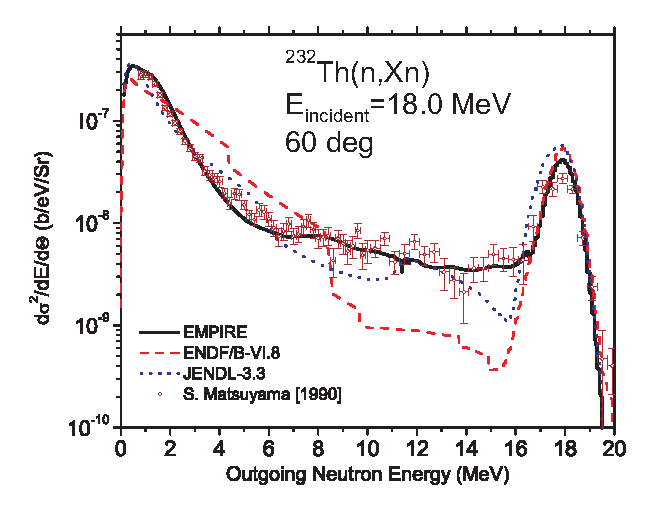
\includegraphics{thorium.eps}}
\caption{EMPIRE calculation for the neutron spectra emission at 60 degree for an incident neutron
 energy of 18.0~MeV on $^{232}$Th, compared to experimental data~\cite{mats} and the ENDF/B-VI.8 and
JENDL-3.3 libraries.}
\label{thoriumMSD}
\end{figure}


\subsubsection{$\gamma$-emission in Multi-step Compound}

The emission of $\gamma$ in the Multi-step Compound\index{MSC} mechanism
is treated in terms of the model proposed by Hoering and Weidenmueller
\cite{GammaMSC}. Application follows the paper by Herman \emph{et
al}. \cite{GammaMSCapp}. The model assumes that $\gamma$ emission
occurs through the deexcitation of the Giant Dipole Resonance (GDR)
built within MSC\index{MSC} classes. Following Brink-Axel hypothesis
\cite{Axel,Brink,Brinka} each nuclear state serves as the basis of
a GDR excitation with identical properties. Moreover, the Tamm-Dancoff
approximation is used and GDR is represented as a linear combination
of correlated 1p-1h states. Each MSC class \emph{M,} now characterized
also by its spin \emph{J,} splits into four sub-classes $M_{n}$.
The states in subclasses $M_{n}$, with \emph{n}=1, 2 and 3 contain
GDR built on states in class \emph{M-1} with spins \emph{J-1, J},
and \emph{J+1}, respectively, and opposite parity. The states in class
$M_{4}$ are pure single particle excitations and contain no GDR.

The pure MSC-contribution to the cross section is obtained while neglecting
the GDR built on the ground state, which leads to the non-statistical
direct-semidirect process. The theory \cite{GammaMSC} allows for
the inclusion of direct-semidirect in the formalism. However, the
implementation of direct-semidirect in the EMPIRE is oversimplified
and has been disabled. On the other hand, an option is provided to
start MSC\index{MSC} calculations right from the first class. This
approach lacks formal justification but brings the model closer to
the treatment of $\gamma$ emission in the classical preequilibrium
models.

The average MSC cross section is given by \begin{equation}
\overline{\sigma_{a,\gamma}^{MSC}}=T_{a,Mm}\Pi_{Mm,Nn}T_{Nn,\gamma},\label{GammaMSCxs}\end{equation}
where \begin{eqnarray}
(\Pi^{-1})_{Mm,Nn} & = & 2\pi\rho_{Mm}v_{Mm,Nn}2\pi\rho_{Nn}\nonumber \\
 &  & +\delta_{M,N}\delta_{m,n}2\pi\rho_{Mm}(\Gamma_{Mm}^{\uparrow}+\Gamma_{Mm}^{\downarrow})\label{Pigamma}\end{eqnarray}
and $T_{a}=\sum_{Mm}T_{aMm}$ are the optical model transmission coefficients.

The transmission coefficients for the \emph{E1}-$\gamma$ channel
are defined, as for the particle channel, in terms of the unitarity
deficit of the average $S$-matrix. \begin{equation}
T_{\gamma}=1-\Big|\overline{S_{\gamma\gamma}}\Big|^{2}.\end{equation}
This is directly proportional to the strength function $f(E)$, which
can be written as a function of the absorption cross section, yielding
\begin{equation}
T_{\gamma}^{E_{1}}=\frac{1}{2\pi}\sigma_{abs}(E_{\gamma}^{E_{1}})\frac{(E_{\gamma}^{E_{1}})^{2}}{(\hbar c)^{2}}.\end{equation}
The absorption cross section has a Lorentzian form and is given by
\begin{equation}
\sigma_{abs}(E_{\gamma}^{E_{1}})=\sigma_{res}\frac{(E_{\gamma}^{E_{1}})^{2}\Gamma_{res}^{2}}{((E_{\gamma}^{E_{1}})^{2}-E_{res}^{2})^{2}+(E_{\gamma}^{E_{1}})^{2}\Gamma_{res}^{2}}.\end{equation}
For the resonance energy $E_{res}$, the resonance width $\Gamma_{res}$,
and the peak cross section $\sigma_{res}$, the experimental or systematics
data are used as input parameters. As in the case of particle emission,
the average matrix element $v_{Mm,Nn}$ coupling non-collective states
of two exciton classes is determined from the imaginary part of the
optical model potential.

Next, we will analyze the individual matrix elements $(\Pi^{-1})_{Mm,Nn}$.
We begin by investigating the non-diagonal block $(\Pi^{-1})_{Mm,(M+1)n}=2\pi\rho_{Mm}v_{Mm,(M+1)n}^{2}2\pi\rho_{(M+1)n}$,
i. e., the transition from a state in exciton class $M$ to a state
in the next higher exciton class $(M+1)$. There are four different
types of matrix elements:

\begin{itemize}
\item decay of a GDR,
\item the single particle transitions leaving the GDR unchanged,
\item transitions among non-collective states,
\item GDR creation.
\end{itemize}
Computation of these four types of matrix elements is discussed below.

\smallskip
\textbf{(i)} The matrix element $(\Pi^{-1})_{Mm,(M+1)4}$, $m=$ 1,
2 or 3 describes the decay of a GDR via coupling to the next higher
exciton class. This process is responsible for the spreading width
of the GDR. In colliding with a bound particle the GDR looses its
coherence and the bound particle is excited into an excited state
thus creating another particle-hole state. This matrix element can
be written as \begin{equation}
2\pi\rho_{Mm}v_{Mm,(M+1)4}^{2}2\pi\rho_{(M+1)4}=2\pi\rho_{Mm}\Gamma_{GDR}^{\downarrow}.\end{equation}
For the width of the GDR the experimental value is used. Unfortunately,
there is little literature on how this width is separated into spreading
and decay width. It is known that for heavy nuclei the spreading width
is dominant, whereas for light nuclei the reverse is true. For $^{208}$Pb
approximately 90\% of the width is due to the spreading width. For
$^{16}$O, on the other hand, 90\% of the width is due to the decay
width \cite{BBB83}. This separation can be entered into the calculations
as an input parameter. The result depends only weakly on this coefficient.
The level densit\index{p-h level density}ies $\rho_{Mm}^{J,\pi}(E)$
for m=1,2,3 are given by the exciton level densities $\rho_{M-1}^{(J-1),-\pi}(E-E_{GDR})$,
$\rho_{M-1}^{J,-\pi}(E-E_{GDR})$ and $\rho_{M-1}^{(J+1),-\pi}(E-E_{GDR})$,
respectively. These correspond to the level densities of the non-collective
states on which GDR is built. Implicitly, all of them are for bound
configurations.

\smallskip
\textbf{(ii)} The matrix element $(\Pi^{-1})_{Mm,(M+1)n}$, m, n=1,
2, 3 describes the transition of a GDR-state in class $M$ to a GDR-state
in class $(M+1)$. In such a transition the GDR is not affected and
is just a \char`\"{}spectator\char`\"{}. This is again a consequence
of the two-body nature of the residual interaction. The subclasses
1, 2, 3 differ only in the angular momenta of the non-collective states
the GDR is built on. Since a transition among these states must not
change the angular momentum this part is diagonal in the subclass
indices, i. e. $(\Pi^{-1})_{Mm,(M+1)m}\not=0$, only. Thus, these
matrix elements are given by \begin{equation}
(\Pi^{-1})_{Mm,(M+1)m}=2\pi\rho_{Mm}v_{n.c.}^{2}2\pi\rho_{Mm\rightarrow(M+1)m}^{acc},\end{equation}
where $\rho_{Mm}^{J}(E)$, m=1,2,3, is the exciton level densit\index{p-h level densities}y
$\rho_{M-1}^{(J^{\prime},-\pi)}(E-E_{GDR})$ with $J^{\prime}=(J-1),J,(J+1)$
$\rho_{Mm\rightarrow(M+1)m}^{acc}(E)$, m=1, 2, 3 are the accessible
state densities $\rho_{(M-1),J\rightarrow M,J^{\prime}}^{acc}(E-E_{GDR})$
with $J^{\prime}=(J-1),\,,J,\,(J+1)$, respectively. $v_{n.c.}$ stands
for the average transition matrix element between two non-collective
states of neighboring exciton classes.

\smallskip
\textbf{(iii)} The matrix element $(\Pi^{-1})_{M4,(M+1)4}$ describes
transitions between non-collective states only. The matrix element
is again expressed through the average transition strength $v_{n.c.}$
between two non-collective states \begin{equation}
(\Pi^{-1})_{M4,(M+1)4}=2\pi\rho_{M4}(E)v_{n.c.}^{2}2\pi\rho_{M4\rightarrow(M+1)4}^{acc}(E).\end{equation}

\smallskip
\textbf{(iv)} The matrix element $(\Pi^{-1})_{M4,(M+1)m}$ with $m$
= 1, 2, and 3 describes the creation of a GDR in the next higher exciton
class. In the current version of EMPIRE the total GDR width is taken
to describe this process%
\footnote{This may overestimate creation rate of the GDR. Other approaches are
to use non-collective matrix element or the GDR width split among
the neighboring classes. To activate these possibilities the user
has to edit MSC\index{MSC}-NVWY\index{NVWY}.f file and uncomment
adequate lines in both of the following ranges 1028-1036 and 1093-1106.%
}. However, the creation of a GDR is possible only if a particle or
a hole has enough energy to create the GDR state. This is another
consequence of the two-body nature of the residual interaction. A
particle with the excitation energy of the GDR resonance is generally
unbound. Thus, only a hole can contribute. The probability for a hole
to have the required energy $\epsilon$ within the configuration with
the total exciton number $(p+h)$ is given by \begin{equation}
P(\epsilon)=N\frac{\rho(p,h-1,E-\epsilon)}{\rho(p,h,E)},\end{equation}
where $\rho(p,h-1,E-\epsilon)$ is the level density\index{p-h level densities}
of the remaining excitons after removing a hole of the energy $\epsilon$.
$\rho(p,h,E)$ is the total level density at energy $E$ for $(p+h)$
excitons. $N$ is the normalization constant. \begin{equation}
\frac{1}{N}=\int_{0}^{E}\frac{\rho(p,h-1,E-\epsilon)}{\rho(p,h,E)}d\epsilon=\frac{\rho(p,h-1,E)}{\rho(p,h,E)(p+h-1)}.\end{equation}
Hence, the probability for a hole to have the energy $E\geq E_{GDR}$
is given by \begin{eqnarray}
\int_{E_{GDR}}^{E}P(\epsilon)d\epsilon & = & \frac{(p+h-1)}{\rho(p,h-1,E)}\int_{E_{GDR}}^{E}\rho(p,h-1,E-\epsilon)d\epsilon\nonumber \\
 & = & \frac{\rho(p,h-1,E-E_{GDR})}{\rho(p,h,E)}.\end{eqnarray}
Collecting everything yields \begin{equation}
(\Pi^{-1})_{M4,(M+1)m}=2\pi\rho_{M4}(E)\Gamma_{GDR}^{\downarrow}\frac{\rho(p,h-1,E-E_{GDR})}{\rho(p,h,E)}.\end{equation}


Thus, all four types of matrix elements within the block $(M,M+1)$
have been determined. The matrix element $(\Pi^{-1})_{(M+1)m,Mn}$
is obtained using the symmetry properties of the matrix $\Pi^{-1}$.
The diagonal elements of this matrix are then obtained by summation:
\begin{eqnarray}
(\Pi^{-1})_{Mm,Mm} &=& \sum_{n=1}^{4}(\Pi^{-1})_{Mm,(M+1)n}  \\
&+& \sum_{n=1}^{4}(\Pi^{-1})_{Mm,(M-1)n} + \sum_{c}T_{Mm,c} \hspace{1pt}.\nonumber
\end{eqnarray}
The matrix $\Pi^{-1}$is inverted numerically and used in Eq.\ref{GammaMSCxs}
to calculate $\gamma$-emission spectra.



%%%%%%%%%%%%%%%%%%%%%%%%%%%%%%%%%%%%%%%%%%%%%%%%%%%%%%%%%%%%%%%%%%%%%%%%%%%%%%%%%%%%%%%%%%%%%%%%%%%%%%%%%%%%%%%%%%
\subsubsection{Exciton model DEGAS\label{DEGAS}}

The module DEGAS\index{DEGAS} is the exciton model
code with angular-momentum conservation written by E. B\v et\' ak
as an improved version of the code PEGAS \cite{Degas} by E. B\v et\' ak
and P. Oblo\v zinsk\' y.  Certain features of the DEGAS code
were intentionally disabled for compatibility with other models.
%present in the EMPIRE code.
Thus, $\gamma$-cascade has been limited to primary
$\gamma$s in the composite nucleus and multiple preequilibrium emissions
have been blocked. In particular, DEGAS treatment of the equilibrium
emission was disabled and left to the Hauser-Feshbach\index{Hauser-Feshbach}
model.
% coded in EMPIRE.
Within the above simplifications DEGAS\index{DEGAS} solves the classical
(apart of spin) set of master equations
\begin{eqnarray}
\frac{dP(E,J,n,t)}{dt} & = & P(E,J,n-2,t)\lambda^{+}(E,J,n-2)\nonumber \\
 & + & P(E,J,n+2,t)\lambda^{-}(E,J,n+2)\nonumber \\
 & + & P(E,J,n,t)\left[\lambda^{+}(E,J,n)\right]\nonumber\\
 & + & P(E,J,n,t)\left[\lambda^{-}(E,J,n)+L(E,J,n)\right]\label{mastereq}\nonumber\\
 & + & \sum_{J^{'},n^{'},x}\int P(E^{'},J^{'},n^{'},t)\lambda_{x}\nonumber\\
 &&\text{x} \left(\left[E^{'},J^{'},n^{'}\right]\rightarrow\left[E,J,n\right]\right)d\varepsilon,
\end{eqnarray}
\noindent where $P(E,J,n,t)$ is the occupation probability of the composite
nucleus at the excitation energy $E$, spin $J$ and the exciton number
$n$, $\lambda^{+}$ and $\lambda^{-}$ are the transition rates for
decay to neighboring states, and $L$ is the total integrated emission
rate for particles (protons $\pi$ and neutrons $\nu$) and $\gamma$-rays.
Note, that the last term ensures coupling of different spins. The
nucleon emission rate per energy and time is
\begin{eqnarray}
\lambda_{\pi,\nu}\left(\left[E,J,n\right]\rightarrow\left[U,S,n-1\right]\right)&=&\\
\frac{1}{h}\frac{\omega(n-1,U,S)}{\omega(n,E,J)}\Re_{\pi,\nu}(n)&\text{x}& \sum_{j=\mid S-1/2\mid}^{S+1/2}\sum_{l=\mid J-j\mid}^{J-j}T_{l}(\varepsilon),\nonumber
\end{eqnarray}
\noindent where $\omega(n,E,J)$ is the particle-hole state density, $T_{l}$s
are the transmission coefficients of the emitted nucleon, and $\Re_{x}(n)$
is a fraction of $x$-type nucleons in the $n$-th stage. The particle-hole
state density is
\begin{equation}
\omega(n,E,J)=\frac{g(gE-A_{p,h})^{n}}{p!h!(n-1)!}R_{n}(J),
\end{equation}
\noindent where $g$ is the single-particle level density\index{p-h level densities}y,
$p$ and $h$ are number of particles and holes ($n=p+h$), and $A_{p,h}$
is the Pauli correction term. The spin distribution reads
\begin{equation}
R_{n}(J)=\frac{2J+1}{2}exp\left(-\frac{(J+1/2)^{2}}{2\sigma_{n}^{2}}\right),
\end{equation}
 with $\sigma_{n}$ being the spin cut-off parameter ($\sigma_{n}^{2}=(0.24+0.0038\cdot E)\cdot nA^{2/3}).$
Treatment of the intranuclear cascade rates follows the FKK \cite{FKK}
approach. The energy and spin dependence are assumed to factorize
\begin{equation}
\lambda^{\pm}(E,J,n)=\frac{2\pi}{\hbar}|M|^{2}Y_{n}^{\downarrow}X_{nJ}^{\downarrow},
\end{equation}
\noindent where $|M|^{2}$ is the energy part of the average squared transition
matrix element of the residual interaction, $Y_{n}^{\downarrow}$
is the energy part of the density of accessible final states,  and
the $X_{nJ}^{\downarrow}$ factor takes care of angular momentum coupling.
The latter two read
\begin{equation}
Y_{n}^{\downarrow}=\frac{g}{2(n+1)}\frac{(gE-A_{p+1,h+1})^{n+1}}{(gE-A_{ph})^{n-1}},
\end{equation}
 and
\begin{equation}
X_{nJ}^{\downarrow}=\frac{1}{R_{n}(J)}\sum_{j_{4}Q}R_{1}(Q)\widetilde{F}(Q)R_{n-1}(j_{4})\Delta(Qj_{4}J),
\end{equation}
 with $\Delta(Qj_{4}J)=1$ for $|Q-j_{4}|\leq J\leq Q+j_{4}$ and
0 otherwise. The function $\widetilde{F}(Q)$ is given by
\begin{equation}
\widetilde{F}(Q)=\sum_{j_{3}j_{5}}(2j_{5}+1)R_{1}(j_{5})(2j_{3}+1)F(j_{3})\left(\begin{array}{ccc}
j_{5} & j_{3} & Q\\
\frac{1}{2} & 0 & -\frac{1}{2}\end{array}\right)^{2},
\end{equation}
 and the angular momentum density of the pair of states is
\begin{equation}
F(j_{3})=\sum_{j_{1}j_{2}}(2j_{1}+1)R_{1}(j_{1})(2j_{2}+1)R_{1}(j_{2})\left(\begin{array}{ccc}
j_{1} & j_{2} & j_{3}\\
\frac{1}{2} & -\frac{1}{2} & 0\end{array}\right)^{2}.
\end{equation}
The averaged squared matrix element $|M|^{2}$ is related to the spin-independent
estimate of Kalbach \cite{Kalbach}
\begin{equation}
|M_{nonspin}|^{2}=KA^{-1/3}\varepsilon^{-1},
\end{equation}
\noindent where $\varepsilon=E/n$ is the energy per single exciton. The more
complicated expressions \cite{Kalbach} are used if $\varepsilon$
is outside the 7-15 MeV range. In the current, spin-dependent formulation
the averaged squared matrix element is chosen in such a way that,
after performing additional averaging over spin, the non-spin value
is recovered
\begin{equation}
|M|^{2}\left\langle X_{nJ}^{\downarrow}\right\rangle =|M_{\text{non spin}}|^{2}.
\end{equation}
\begin{figure}[htbp]
\scalebox{0.8}{\includegraphics{ir193.eps}}
\caption{Neutron capture cross section for $^{193}$Ir. }
\label{ir193}
\end{figure}

For the $K$ constant the standard value of 100 MeV$^{3}$ is adopted.
The coding of $\gamma$-emission makes use of the Brink-Axel hypothesis
\cite{Axel,Brink,Brinka} and Giant Dipole Resonance $\gamma$-ray
strength function for the $E1$ transitions. In the angular momentum
coupling formalism the $\gamma$ emission rate $\lambda_{\gamma}$
from an $n$-exciton state is
\begin{eqnarray}
\lambda_{\gamma}\left(\left[E,J,n\right]\rightarrow\left[E-E_{\gamma},S,n\right]\right)&=&\\
\frac{E_{\gamma}^{2}\sigma_{GDR}(E_{\gamma})}{3\pi^{2}\hbar^{3}c^{2}}&\times&\frac{b_{nS}^{nJ}\omega(n,E-E_{\gamma},S)}{\omega(n,E,J)}
\nonumber,
\end{eqnarray}
 if emission of a $\gamma$ occurs with no change in the exciton number,
or
\begin{eqnarray}
\lambda_{\gamma}\left(\left[E,J,n\right]\rightarrow\left[E-E_{\gamma},S,n-2\right]\right)&=&\nonumber\\
\frac{E_{\gamma}^{2}\sigma_{GDR}(E_{\gamma})}{3\pi^{2}\hbar^{3}c^{2}}&\times&\nonumber\\
\frac{b_{n-2,S}^{nJ}\omega(n-2,E-E_{\gamma},S)}{\omega(n,E,J)},&&
\end{eqnarray}
 in the case of annihilation of one particle-hole pair. The photoabsorption
cross section $\sigma_{GDR}(E_{\gamma})$ is written in the Lorentzian
form
\begin{equation}
\sigma_{GDR}(E_{\gamma})=53.2mb\frac{NZ}{A}\frac{E_{\gamma}^{2}\Gamma^{2}}{\left(E_{\gamma}^{2}-E_{GDR}^{2}\right)^{2}+E_{\gamma}^{2}\Gamma^{2}},
\end{equation}
with $\Gamma=5$ MeV and
\begin{equation}
E_{GDR}=29\sqrt{\left(1+2/A^{1/3}\right)/A^{1/3}}\,\,[MeV].
\end{equation}
 The branching ratios are
\begin{equation}
b_{nS}^{nJ}=\frac{y_{m}^{n}x_{mS}^{nJ}}{y_{m}^{m}x_{mS}^{mJ}+y_{m}^{m+2}x_{mS}^{m+2,J}},
\end{equation}
\noindent where
\begin{eqnarray}
y_{n}^{n} & = & gn,\nonumber \\
y_{n}^{n+2} & = & g^{2}\varepsilon,
\end{eqnarray}
and the spin coupling terms read
\begin{eqnarray}
x_{nS}^{nJ} & = & \frac{3(2J+1)}{R_{n}(S)}\nonumber\\
& \times &\sum_{j_{1}j_{2}j_{3}}(2j_{1}+1)R_{1}(j_{1})(2j_{2}+1)R_{1}(j_{2})R_{n-1}(j_{3})\nonumber \\
 & \times & \left(\begin{array}{ccc}
j_{2} & 1 & j_{1}\\
\frac{1}{2} & 0 & -\frac{1}{2}\end{array}\right)^{2}\left\{ \begin{array}{ccc}
j_{2} & j_{3} & S\\
J & 1 & j_{1}\end{array}\right\} ^{2}
\end{eqnarray}
and
\begin{eqnarray}
x_{nS}^{n+2,J}&=&\frac{2J+1}{2S+1}\nonumber\\
&\times&\sum_{j_{1}j_{2}}(2j_{1}+1)R_{1}(j_{1})(2j_{2}+1)R_{1}(j_{2})\nonumber\\
&\times&\left(\begin{array}{ccc}
j_{2} & j_{1} & 1\\
\frac{1}{2} & -\frac{1}{2} & 0\end{array}\right)^{2}\Delta(S1J).
\end{eqnarray}
DEGAS\index{DEGAS} solves the set of master equations (Eq. \ref{mastereq})
and calculates integrals of occupation probabilities
\begin{equation}
\tau(E,J,n)=\int_{0}^{\infty}P(E,J,n,t)dt,
\end{equation}
and preequilibrium emission cross sections
\begin{eqnarray}
\frac{d\sigma_{x}}{d\varepsilon_{x}}&=&\sum_{J_{c},J_{r},n}\int\sigma(E_{c},J_{c})\tau(E_{c},J_{c},n)\lambda_{x}\nonumber\\
&\times&\left(\left[E_{c},J_{c},n\right]\rightarrow\left[E_{r},J_{r},n-1\right]\right)dE_{r}.
\end{eqnarray}
Here, subscripts $c$ and $r$ refer to the composite and residual
nuclei respectively.

An example of an improved calculation of neutron capture reaction on $^{193}$Ir is presented
in Fig.~\ref{ir193}. Two calculations, with and without the DEGAS modelization shows the increase
of the capture cross section above 3~MeV.



\subsubsection{Exciton model PCROSS\label{PCROSS}}
The module PCROSS includes a preequilibrium mechanism for clusters in the incoming and outgoing
channels by including the Iwamoto-Harade model~\cite{Iwamoto} parameterized and improved
in~\cite{Sato,Zhang1,Zhang2}. In this model, the formation probability of a cluster takes into
account excitons below and above the Fermi surface and avoids free parameters. In Fig.~\ref{goldna},
the Iwamoto-Harada model brings an essential improvement into the treatment of the $\alpha$-particle
 emission in the $^{197}$Au(n,$\alpha$) reaction.
\begin{figure}[htbp]
\scalebox{0.61}{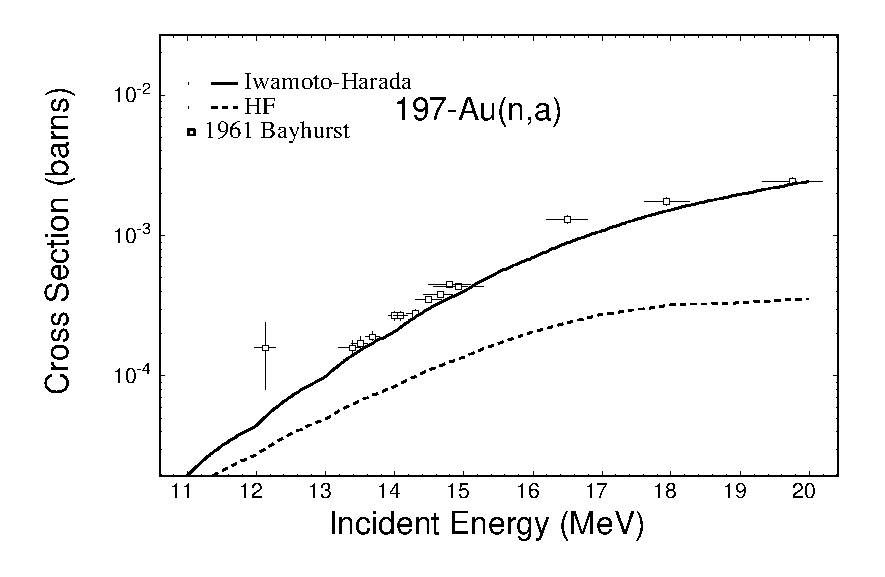
\includegraphics{hermanm1_f4.eps}}
\caption{Improvement achieved with the Iwamoto-Harada model for $^{179}$Au(n,$\alpha$) reaction.}
\label{goldna}
\end{figure}




%%%%%%%%%%%%%%%%%%%%%%%%%%%%%%%%%%%%%%%%%%%%%%%%%%%%%%%%%%%%%%%%%%%%%%%%%%%%%%%%%%%%%%%%%%%%%%%%%%%%%%%%%%%%%%%%%%
\subsubsection{Monte Carlo Preequilibrium\label{DDHMS}}
The Hybrid Monte-Carlo Simulation (HMS) approach to the preequilibrium
emission of nucleons  has
been formulated by M. Blann \cite{Blann-HMS} as a hybrid model
\cite{hybrid,hybrid1,hybrid2,hybrid3}
inspired version of the intranuclear cascade approach. Contrary to
other classical preequilibrium models, this approach avoids multi-exciton
level densities\index{p-h level densities}, which were shown by Bisplinghoff
\cite{Bisplinghoff} to be used inconsistently in the exciton and
in the hybrid formulations. The HMS\index{HMS} model has a number
of attractive features. First of all, there are no physical limits
on a number of preequilibrium emissions (apart from energy conservation).
With the addition of linear momentum conservation by M. Chadwick and
P. Oblo\v zinsk\' y (DDHMS), the model provides a nearly complete
set of observables. These include cross sections for the production
of residuals, light-particle double-differential spectra and spectra
of recoils. Spin and excitation-energy dependent populations of residual
nuclei can also be obtained, an essential feature for coupling the
preequilibrium mechanism to the subsequent Compound Nucleus decay.
The binding energies in the HMS\index{HMS} model are thermodynamically
correct. The DDHMS model proved to perform very well
%up to at least 250 MeV, extending energy range of the EMPIRE applicability
up to at least 250 MeV.
%to the desired limit.
The calculation flow in the DDHMS model can be summarized in terms
of the following steps:
\begin{enumerate}
\item draw collision partner for the incoming nucleon (2p-1h state created)
\item draw energy ($\varepsilon$) of the scattered nucleon (if bound go
to step 5)
\item draw scattering angles for both particles
\item decide whether the scattered nucleon will be emitted, re-scattered
or trapped
\begin{enumerate}
\item if emitted appropriate cross section is augmented
\item if re-scatters additional particle-hole is created and we return to
step 2
\item if trapped, go to step 5
\end{enumerate}
\item draw excitation energy of a particle in the remaining 1p-1h configuration
(between 0$\div(U-\varepsilon)$), if unbound go to step 3, if bound
choose another existing 1p-1h pair and repeat step 5.
\end{enumerate}

\begin{figure}[htbp]
\scalebox{0.75}{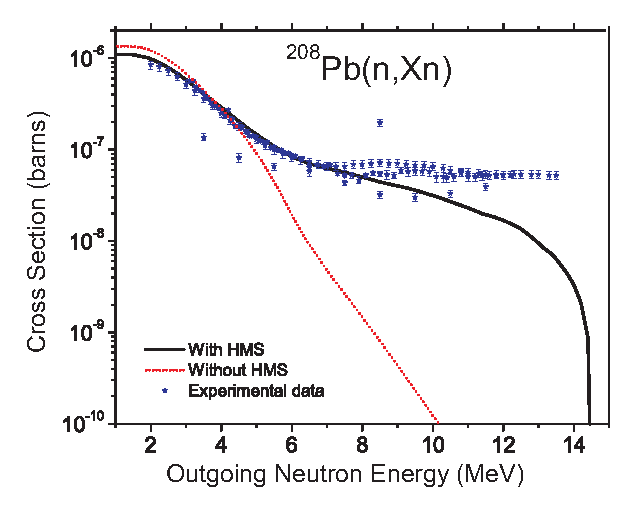
\includegraphics{pb208.eps}}
\caption{Neutron emission for $^{208}$Pb(n,xn) reaction with and without HMS.}
\label{pb208HMS}
\end{figure}




All excitons (including holes) are treated on equal footing and each
of them is given a chance to interact or being emitted with \emph{a
priori} equal probability. The cascade ends when all excitons are
bound. Below, we summarize various probability distributions which
are used in concert with a random number generator.
For choosing a collision partner it is assumed that the unlike interaction
is 3 times more probable than the like one ($\sigma_{np}=3\sigma_{nn}$).
Thus, for the incident neutron we have $P_{nn}$ and $P_{np}$ for
the probability of exciting neutron and proton respectively
\begin{equation}
P_{nn}=\frac{(A-Z)}{(A-Z)+3Z},\label{Pnn}\end{equation}

\begin{equation}
P_{np}=1-P_{nn}\label{Pnp}\end{equation}
 and similarly for the incident proton
\begin{equation}
P_{pp}=\frac{Z}{Z+3(A-Z)},\label{Ppp}\end{equation}
\begin{equation}
P_{pn}=1-P_{pp}.\label{Ppn}\end{equation}
The energy distribution of the scattered particles $P(\varepsilon)$
is given by the ratio of the $(n-1)-$ and $n$-exciton level densities\index{p-h level densities}
$\rho_{n}$
\begin{equation}
P(\varepsilon)d\varepsilon=\frac{\rho_{n-1}(E-\varepsilon)g}{\rho_{n}(E)}d\varepsilon,\label{Penergy}\end{equation}
with $n=2\, or\,3$ and\begin{equation}
\rho_{2}(E)=\frac{g(gV)}{2}\,\,\, if\,\,\, E>V,\label{ro2u}\end{equation}
\begin{equation}
\rho_{2}(E)=\frac{g(gE)}{2}\,\,\, if\,\,\, E\leq V,\label{ro2d}\end{equation}
\begin{equation}
\rho_{3}(E)=\frac{g^{3}\left[V(2E-V)\right]}{4}\,\,\, if\,\,\, E\geq V.\label{ro3}\end{equation}
 Here, $V$ is a potential well depth. The emission probability is
calculated as
\begin{equation}
P_{\nu}(\varepsilon-Q)=\frac{\lambda_{c}(\varepsilon-Q)}{\lambda_{c}(\varepsilon-Q)+\lambda_{+}(\varepsilon)},\label{Pnu}\end{equation}
with the emission rate being
\begin{equation}
\lambda_{c}(\varepsilon-Q)\sim\frac{\sigma_{\nu}(\varepsilon-Q)(\varepsilon-Q)(2S+1)\mu_{\nu}}{g}.\label{lambdac}\end{equation}
$\sigma_{\nu}$ is an inverse reaction cross section, $Q$ is a binding
energy, $g$ is a single particle density, $S$ denotes nucleon spin,
and $\mu_{\nu}$ stands for the reduced nucleon mass. Following the
hybrid\index{HYBRID} model, $\lambda_{+}(\varepsilon)$ is calculated
from the mean free path of a nucleon in nuclear matter.
The version which is actually implemented in EMPIRE has been coded
by M. Chadwick and extended to double-differential cross sections
in collaboration with P. Oblo\v zinsk\' y \cite{DDHMScode}.

Figure~\ref{pb208HMS} presents two calculations, with and without (compound nucleus only) the HMS model for the
neutron emission on $^{208}$Pb at an incident neutron energy of 14.6~MeV. A good agreement is obtained in the
case of the HMS calculation.

\subsubsection{Compatibility of Preequilibrium Models}
Possible inclusions of different preequilibrium models in a single
calculation run rises a problem of double-counting. The current version
of EMPIRE has 5 modules for preequilibrium decay: MSD,
MSC, DEGAS and HMS and PCROSS.
While MSD and MSC describe different reaction mechanisms and are complementary,
neither of them is compatible with DEGAS, HMS or PCROSS. Therefore,
neither of the latter three can be used together with MSD or MSC in
the same exit channel. Also DEGAS, HMS and PCROSS mutually exclude
each other. However, these models can be combined if used in different
exit channels, e.g., neutron inelastic scattering may be calculated
using MSD\&MSC while the emission of protons can be treated within
the exciton model using PCROSS. We also note that summing $\gamma$-emission
spectra from more than one of the three possible mechanisms (MSC,
DEGAS, and PCROSS) would be obvious
multiple-counting and must be avoided.
An additional complication is introduced by the possibility of using
ECIS03, which calculates Coupled-Channel
or DWBA contributions to the collective discrete levels. In general, these
contributions are so strong that adding those provided by the exciton
model leave the results practically unchanged. Thus, ECIS03 can be
considered compatible with HMS since the latter does not include
collective excitations. By the same token ECIS03 is not
compatible with MSD as both include collectivity of discrete
levels. However, ECIS03 and MSD can be combined providing that only
the continuum contribution from the MSD is retained.
To avoid double-counting when combining different models EMPIRE applies
the following priorities:
\begin{description}
\item [ECIS03] provides inelastic scattering to collective
levels independently of the settings for the remaining models.
\item [MSD] provides inelastic continuum independently of other
settings. It also provides vibrational inelastic to discrete levels unless
it is suppressed by the active ECIS03 option.
A user, at his own discretion, may retain MSD contribution and sum it
up with the results of the CC calculations. This option might be physically
acceptable for deformed nuclei to account for both rotational (CC) and
vibrational (MSD) contributions. Note the provision for the second-chance preequilibrium
emission after MSD.
\item [MSC] results are taken for the inelastic to the continuum.
Charge-exchange to the continuum is accepted if not suppressed by
use of DEGAS, HMS or PCROSS.
\item [PCROSS] provides inelastic and charge-exchange to
the continuum if MSD and MSC are not active. Provides $\gamma$-emission if not suppressed by $\gamma$-emission
from MSC or DEGAS. Provides preequilibrium emission of clusters independently
of settings for other models.
\item [DEGAS] provides inelastic and charge-exchange to  the
continuum if these are not provided by any of the above listed
models. Gamma emission from DEGAS overwrites that from PCROSS and
is used if not provided by the MSC.
\item [HMS] provides inelastic and charge-exchange to the continuum
and to discrete levels if MSD and MSC are
not active. Otherwise only the charge-exchange contribution is used.
Suppresses DEGAS and PCROSS results for particle emission if such
was calculated. HMS does not provide $\gamma$-rays, thus
MSC, DEGAS or PCROSS results (in this order!) are adopted.
\end{description}
This scheme allows the user to activate any combination of reaction
mechanisms while the code ensures the internal consistency of calculations.
Overlapping contributions from various models are summed up and the
Compound Nucleus contribution is added in all cases. A concise summary
explaining use of the models is printed as a table at the beginning
of the EMPIRE output. An example is reproduced below:

\begin{verbatim}
Use of preequilibrium models
-------------------------------------------
Exit channel ECIS MSD MSC DEGAS HMS PCROSS
neut. disc.   0    1   0    0    0    0
neut. cont.   0    1   1    0    0    0
prot. disc.   0    0   0    0    0    1
prot. cont.   0    0   0    0    0    1
gammas        0    0   0    1    0    0
alpha cont.   0    0   0    0    0    1
-------------------------------------------
\end{verbatim}

\noindent 1 indicates that the contribution of the model is included,
and 0 means that it is not calculated or ignored. In the above example,
MSD\index{MSD}, MSC\index{MSC}, DEGAS\index{DEGAS} and PCROSS\index{PCROSS}
were invoked, and priority rules caused PCROSS neutron contribution
to be suppressed as well as all DEGAS contributions except emission
of gammas.
Selecting DIRECT =1 (or 2 or 3), MSD=1, MSC=1, PCROSS=1 is supposed
to give the best results at low incident energies (say up to 30 MeV).
At higher incident energies the preference should be given to the
HMS\index{HMS} model, which accounts for the multiple preequilibrium
emission. When selecting appropriate models the user should take into
account that not all of them provide the same set of observables.
In particular, DEGAS\index{DEGAS} is missing angular distributions,
which are calculated by thePCROSS and HMS. On the other hand, preequilibrium
$\gamma$-emission can be obtained from DEGAS, PCROSS or MSC
but not from HMS. Finally, we note that DEGAS is the only $\gamma$-emission
preequilibrium model with proper angular momentum coupling.


\subsubsection{\label{sec:photonuclear} Photonucler reactions}
A model of photonuclear reactions must account for the different reaction
mechanisms involved in the initial photonuclear excitation process
and the subsequent decay of the excited nucleus by particle and gamma-ray
emission. At low energies, below about 30 MeV, the Giant Dipole Resonance
(GDR) is the dominant excitation mechanism, where a collective bulk
oscillation of the neutrons against the protons occurs. At higher
energies, up to approximately 150 MeV, photoabsorption on a neutron-proton
pair (a quasi-deuteron, QD), which has a large dipole moment, is the
dominant mechanism.
In EMPIRE, the photoabsorption cross section is calculated as the
sum of two components~\cite{PHNuc},
\begin{equation}
\sigma_{abs}(E_{\gamma})=\sigma_{GDR}(E_{\gamma})+\sigma_{QD}(E_{\gamma}).
\end{equation}
The GDR component, $\sigma_{GDR}(E_{\gamma})$, is given by a Lorentzian
shape, with parameters describing the total absorption of the giant
dipole resonance. The expression used is given in detail in 2.9.5,
but takes the basic form
\begin{equation}
\sigma_{GDR}(E_{\gamma})=\sum_{i}\sigma_{i}\frac{(E_{\gamma}\Gamma_{i})^{2}}{(E_{\gamma}^{2}-E_{i}^{2})^{2}+(E_{\gamma}\Gamma_{i})^{2}}\,,
\end{equation}
\noindent where $\sigma_{i}$, $E_{i}$ and $\Gamma_{i}$ are the GDR peak cross
section, energy and width, respectively. The summation is limited
to $i=1$ for spherical nuclei, while for deformed nuclei the resonance
is split and one uses $i=1,2$. As a rule, the parameters are derived
from fits to experimental data or from systematics~\cite{RIPL2}.
The QD component, $\sigma_{QD}(E_{\gamma})$, is taken from the model
of Chadwick~\emph{et al.}~\cite{chadQD}, which uses a Levinger-type
theory. It relates the nuclear photoabsorption cross section to the
experimental deuteron photodisintegration cross section, $\sigma_{d}(E_{\gamma})$,
as
\begin{equation}
\sigma_{QD}(E_{\gamma})=L\frac{NZ}{A}\sigma_{d}(E_{\gamma})\, f(E_{\gamma})\,.
\end{equation}
Here, the Levinger parameter was derived as $L=6.5$ and $f(E_{\gamma})$
is the Pauli-blocking function, which reduces the free deuteron cross
section $\sigma_{d}(E_{\gamma})$ to account for Pauli blocking of
the excited neutron and proton by the nuclear medium. The experimental
deuteron photodisintegration cross section was parametrized as
\begin{equation}
\sigma_{d}(E_{\gamma})=61.2\frac{(E_{\gamma}-2.24)^{3/2}}{E_{\gamma}^{3}}\,,
\end{equation}
with $E_{\gamma}$ in MeV and $\sigma_{d}$ in mb. The Pauli-blocking
function was found by Chadwick \emph{et al.} to be a multidimensional
integral whose solution could be well approximated in the energy range
20 -- 140 MeV by the polynomial expression
\begin{eqnarray}
f(E_{\gamma}) & = & \;8.3714\times10^{-2}-9.8343\times10^{-3}E_{\gamma}\nonumber\\
&+&4.1222\times10^{-4}E_{\gamma}^{2} -3.4762\times10^{-6}E_{\gamma}^{3}\nonumber\\
&+&9.3537\times10^{-9}E_{\gamma}^{4}\,,
\end{eqnarray}
with $E_{\gamma}$ in MeV. In Ref.~\cite{chadQD}, the Pauli-blocking
function was not parametrized below 20 MeV, where it tends to zero,
or above 140 MeV, where it tends to unity. As the contribution need
to be defined at all energies considered, EMPIRE follows the example
of Ref.~\cite{PHNuc} and uses an exponential shape, $f(E_{\gamma})=\exp(-D/E_{\gamma})$,
for energies below 20 MeV and above 140 MeV, with $D=73.3$ MeV for
$E_{\gamma}<20$ MeV and $D=24.2$ MeV for $E_{\gamma}>140$ MeV.
This form has the correct behavior in that it tends to zero at $E_{\gamma}=0$
and to unity for large $E_{\gamma}$, and is continuous with the previous
equation at 20 and 140 MeV.
Preequilibrium reaction mechanisms become important for incident photon
energies above 10 to 15 MeV. In the photoabsorption mechanisms described
above, the initial nuclear excitation can be understood in terms of
particle-hole excitations ($1p1h$ for the GDR; $2p2h$ or $2p1h$
for QD processes) and thus it is natural to use a preequilibrium theory
of particle-hole processes to describe the preequilibrium emission
and damping to equilibrium during the evolution of the reaction. Such
models can be used to calculate photonuclear reactions for incident
photons with energies up to about 140 MeV, which is the threshold
for pion production.
\begin{figure}[htbp]
\scalebox{0.16}{\includegraphics{u235abs.eps}}
\caption{Comparison of EMPIRE calculation and experimental data for
photo-absorption on $^{235}$U.}
\label{u235abs}
\end{figure}

At present, EMPIRE permits the calculation of
preequilibrium emission in photonuclear reactions using either the
exciton model module PCROSS\index{PCROSS} or the Hybrid Monte-Carlo
Simulation module HMS\index{HMS}. Both implementations of photoabsorption
represent the GDR fraction as an initial $1p1h$ excitation and the
QD fraction as an initial $2p2h$ excitation. The implementation of
photoabsorption in PCROSS does not take into account the correlation
of the two holes created through the QD mechanism, which would require
an initial configuration closer to a $2p1h$ one than to a $2p2h$
one~\cite{PHNuc}. The implementation in HMS takes this correlation
into account in a manner consistent with the model of Ref.~\cite{chadQD}.
Following the possible emission of preequilibrium particles, the remaining
nuclear system reaches equilibrium, after which it decays by sequential
particle or gamma-ray emission (or possibly fission) until the nuclear
ground state is reached. In EMPIRE, the Hauser-Feshbach theory is
used to calculate cross sections for these processes.
Much more information on photonuclear reactions can be found in
Ref.~\cite{PHNuc}, which served as the basis for this brief description
of these processes.
For illustration of the capability of the EMPIRE code, figure~\ref{u235abs}
compares calculated and experimental photo-absorption
cross sections on $^{235}$U using ML01 $\gamma$-ray strength
function~\cite{mike2}.



%%%%%%%%%%%%%%%%%%%%%%%%%%%%%%%%%%%%%%%%%%%%%%%%%%%%%%%%%%%%%%%%%%%%%%%%%%%%%%%%%%%%%%%%%%%%%%%%%%%%%%%%%%%%%%%%%%
\subsection{Compound Reactions}


%The statistical model used in the EMPIRE is an advanced implementation
The statistical model used in the EMPIRE is an advanced implementation
of the Hauser-Feshbach\index{Hauser-Feshbach} theory. The exact angular
momentum and parity coupling is observed. The emission of neutrons,
protons, $\alpha$-particles, and a light ion is taken into account
along with the competing fission channel. The full $\gamma$-cascade
in the residual nuclei is considered. Particular attention is dedicated
to the determination of the level densities\index{level densities},
which can be calculated in the non-adiabatic approach allowing for
the rotational and vibrational enhancements. These collective effects
are gradually removed above a certain energy. Level densities acquire
dynamic features through the dependence of the rotational enhancement
on the shape of a nucleus.
In the frame of the statistical model of nuclear reactions the contribution
of the Compound Nucleus (CN) state $a$ with spin $J$, parity $\pi$,
and excitation energy $E$ to a channel $b$ is given by the ratio
of the channel width $\Gamma_{b}$ to the total width $\Gamma_{tot}=\sum_{c}\Gamma_{c}$
multiplied by the population of this state $\sigma_{a}(E,J,\pi)$.
This also holds for secondary CNs that are formed due to subsequent
emissions of particles. The only difference is that while the first
CN is initially excited to the unique (incident channel compatible)
energy, the secondary CNs are created with excitation energies which
spread over the available energy interval. Each such state contributes
\noindent
\begin{equation}
\sigma_{b}(E,J,\pi)=\sigma_{a}(E,J,\pi)\frac{\Gamma_{b}(E,J,\pi)}{\sum_{c}\Gamma_{c}(E,J,\pi)}
\label{Hauser}
\end{equation}
\noindent to the cross section. These have to be summed over spin $J$ and parity
$\pi$, and integrated over excitation energy $E$ (in case of daughter
CN) to obtain observable cross sections. The particle decay width
is given by
\begin{eqnarray}
\Gamma_{c}(E,J,\pi)&=&\frac{1}{2\pi\rho_{CN}(E,J,\pi)}\nonumber\\
&\times&\sum_{J'=0}^{\infty}\sum_{\pi'}\sum_{j=J'-J}^{J+J'}\int_{0}^{E-B_{c}}\rho_{c}(E',J',\pi')\nonumber\\
&\times&T_{c}^{l,j}(E-B_{c}-E')dE',\label{pwidth}
\end{eqnarray}
\noindent where $B_{c}$ is the binding energy of particle $c$ in
the compound nucleus, $\rho$ is the level density\index{level density},
and $T_{c}^{l,j}(\epsilon)$ stands for the transmission coefficient
for particle $c$ having channel energy $\epsilon=E-B_{c}-E'$ and
orbital angular momentum $l$, which together with the particle spin
$s$ couples to the channel angular momentum $j$. For the discrete
levels (characterized by the energy $E_{i}$, spin $J_{i}$, and parity
$\pi_{i}$) the level density $\rho(E,J',\pi')$ reduces to $\delta(E-E_{i})\delta_{(J',J_{i})}\delta_{(\pi',\pi_{i})}$.
The parity selection rules are implicit in
Eq. \ref{pwidth}.

\subsubsection{Level densities}
EMPIRE accounts for various models describing level densities\index{level densities}
and includes several respective parameterizations. In each case equal
parity distribution $\rho(E,J,\pi)=\frac{1}{2}\rho(E,J)$ is assumed.
Choice of the proper representation depends on a case being considered.
For the nucleon induced reactions, with CN excited up to about 20
MeV, the Gilbert-Cameron approach is recommended. It assures the most
accurate description of level densities in the energy range up to
the neutron binding energy. The collective effects are included in
the level density parameter $a$, providing reasonable estimate of
the level densities as long as damping of the collective effects is
irrelevant. The relatively low angular momentum introduced by the
incident projectile justifies neglect of dynamical effects.

\paragraph{Gilbert-Cameron level densities}
The Gilbert-Cameron approach \cite{gc} splits excitation energy in
two regions. Different functional forms of level densities\index{level densities}
are applied in each of them. At low excitation energies (below the
matching point $U_{x}$) the constant temperature formula is used
\begin{equation}
\rho_{T}(E)=\frac{1}{T}exp\left[(E-\Delta-E_{0})/T\right],
\label{lgcld}
\end{equation}
\noindent where $T$ is the nuclear temperature, $E$ is the excitation energy
($E=U+\Delta$ with $\Delta$ being the pairing correction), and $E_{0}$
is an adjustable energy shift. Above $U_{x}$ the Fermi gas formula
is applied
\begin{equation}
\rho_{F}(U)=\frac{exp(2\sqrt{aU})}{12\sqrt{2}\sigma^3(U)a^{1/4}U^{5/4}}.
\label{ferld}
\end{equation}
The level density parameter $a$ is assumed to be energy independent.
The spin cut-off factor $\sigma(U)$ is given by
\begin{equation}
\sigma^{2}(U)=0.146A^{2/3}\sqrt{aU}.
\label{sigld}
\end{equation}
Three model parameters, $T,\, U_{x},$ and $E_{0}$, are determined
by the requirement that the level density and its derivative are continuous
at the matching point $U_{x}$, and by fitting cumulative number of
discrete levels with the integral of Eq. \ref{lgcld}. The first of
the conditions implies
\begin{equation}
\frac{1}{T}=\sqrt{a/U_{x}}-\frac{3}{2U_{x}}.
\label{condUT}
\end{equation}
The systematics of the level density parameter $a$ used by EMPIRE,
account for the shell effects, which fade-out
with increasing energy implying energy dependence of the $a$ parameter.
The general form of this dependence was proposed by Ignatyuk~\cite{ignaa}
\begin{equation}
a(U)=\widetilde{a}[1+f(U)\frac{\delta W}{U}],
\label{apiccoloGC}
\end{equation}
\noindent where $\delta W$ is the shell correction, $\widetilde{a}$ is the
asymptotic value of the $a$-parameter and
\begin{equation}
f(U)=1-exp(-\gamma U).
\label{shellGC}
\end{equation}
The three relevant systematics available in EMPIRE are:
\begin{description}
\item[Ignatyuk~\emph{et al.}~\cite{ignaa}]: $\widetilde{a}=0.154A+6.3\cdot10^{-5}A^{2}$
and $\gamma=-0.054$
\item[Arthur~\cite{arthura}]: $\widetilde{a}=0.1375A-8.36\cdot10^{-5}A^{2}$
and $\gamma=-0.054$
\item[Iljinov~\emph{et al.}~\cite{Mebel}]: $\widetilde{a}=0.114A+9.80\cdot10^{-2}A^{2/3}$
and $\gamma=-0.051$
\end{description}
We stress that Gilbert-Cameron approach does not account explicitly
for the collective enhancements of the level densities\index{level densities}.
These are included implicitly in the $\widetilde{a}$ when fitting
neutron resonance spacings. Such an approach leads to the over-estimation
of the level densities above, say, 20 MeV.

\paragraph{EMPIRE-specific level densities}
The dynamic approach to the level densities\index{level densities}
is specific to the EMPIRE code. It takes into account collective enhancements
of the level densities due to nuclear vibration and rotation. The
formalism uses the super-fluid model below critical excitation energy
and the Fermi gas model above. Differently from other
similar formulations, the latter one accounts explicitly for the rotation
induced deformation of the nucleus, which becomes spin dependent.
The deformation enters level densities
formulas through moments of inertia and through the level density
parameter \emph{a} that increases with increase in the surface of
the nucleus.
Assuming that the prolate nuclei rotate along the axis perpendicular
to the symmetry axis the explicit level density formulas reads
\begin{eqnarray}
\rho(E,J,\pi) & = & \frac{1}{16\sqrt{6\pi}}\left(\frac{\hbar^{2}}{\Im_{\Vert}}\right)^{\frac{1}{2}}a^{1/4}\sum_{K=-J}^{J}\left(U-\frac{\hbar^{2}K^{2}}{2\Im_{eff}}\right)^{-\frac{5}{4}}\nonumber \\
 &  & \exp\left\{ 2\left[a\left(U-\frac{\hbar^{2}K^{2}}{2\Im_{eff}}\right)\right]^{\frac{1}{2}}\right\} .\label{ro1}
\end{eqnarray}
In the case of the oblate nuclei which are assumed to rotate parallel
to the symmetry axis we have
\begin{eqnarray}
\rho(E,J,\pi) & = & \frac{1}{16\sqrt{6\pi}}\left(\frac{\hbar^{2}}{\Im_{\Vert}}\right)^{\frac{1}{2}}a^{1/4}\nonumber \\
 &  & \sum_{K=-J}^{J}\left(U-\frac{\hbar^{2}\left[J\left(J+1\right)-K^{2}\right]}{2|\Im_{eff}|}\right)^{-\frac{5}{4}}\label{ro2}\\
 &  & \exp\left\{ 2\left[a\left(U-\frac{\hbar^{2}\left[J\left(J+1\right)-K^{2}\right]}{2|\Im_{eff}|}\right)\right]^{\frac{1}{2}}\right\} .\nonumber
 \end{eqnarray}
$a$ is a level density\index{level density} parameter, $J$ is a
nucleus spin and $K$ its projection, $E$ is the excitation energy
and $U$ is the excitation energy less pairing ($\Delta$). The effective
moment of inertia $\Im_{eff}$ is defined in terms of the perpendicular
$\Im_{\Vert}$and parallel $\Im_{\bot}$moments through the difference
of their inverses
\begin{equation}
\frac{1}{\Im_{eff}}=\frac{1}{\Im_{\Vert}}-\frac{1}{\Im_{\bot}}.\label{mom-iner}
\end{equation}
The saddle-point moments of inertia are calculated using Sierk's routine
MOMFIT \cite{sierk}, which provides a fit to the advanced liquid-drop
model calculations.
It should be stressed that Eqs. \ref{ro1} and \ref{ro2} include
summation over projection of the angular momentum $K$ and thus automatically
account for the rotational enhancement. The yrast line is obtained,
setting level densities to 0 whenever the
rotational energy becomes larger than $U$. In addition to the rotational
enhancement the model accounts also for the vibrational enhancement.
To this end Eqs. \ref{ro1} and
\ref{ro2} are multiplied by $K_{vib}$
\begin{equation}
K_{vib}=exp\left\{ 1.7\left(\frac{3m_{0}A}{4\pi h^{2}S_{drop}}\right)^{2/3}T^{4/3}\right\} \label{Kvib}
\end{equation}
with $S_{drop}=17/4\pi r_{^{2}0}$ and $r_{0}=1.26$.
Damping of the rotational enhancement is achieved by multiplying Eqs.
\ref{ro1} and \ref{ro2} by
\begin{equation}
1-Q_{rot}\left(1-\frac{1}{\hbar^{2}/\Im_{\bot}t}\right)\label{damp}
\end{equation}

\noindent where $Q_{rot}=2/\left[\exp(E_{cor}/t)+1\right]$ is a damping function
which tends to 0 for low temperatures $t$, and approaches 1 for $t\rightarrow\infty$.
The Coriolis energy is given by
\begin{equation}
E_{cor}\simeq\hbar\omega_{0}\mid\delta_{osc}\mid=41A^{-1/3}\mid\delta_{osc}\mid.\label{Coriolis}
\end{equation}


\noindent Following Junghans \emph{et al.} \cite{Ignadamp} $Q_{rot}$
is assumed to be deformation independent
\begin{equation}
Q_{rot}=\frac{1}{1+exp\left(-\frac{E_{cr}}{d_{cr}}\right)}-\frac{1}{1+exp\left(-\frac{E-E_{cr}}{d_{cr}}\right)}\label{Qrot}
\end{equation}
 \noindent with $E_{cr}=40$ MeV and $d_{cr}=10$ MeV. The two terms
in Eq. \ref{Qrot} ensure that $Q_{rot}=0$ at $E=0$ and tends to
1 for $E\rightarrow\infty$. We note that $\hbar^{2}/\Im_{\bot}t$
is approximately equal to the rotational enhancement and therefore
multiplication of the level densities\index{level densities} by Eq.
\ref{damp} actually removes rotational enhancement when $Q_{rot}=1$.
As nuclear temperature $T$ increases the vibrational enhancement
is damped by multiplying Eqs. \ref{ro1} and \ref{ro2} by the factor
\begin{equation}
Q_{vib}=exp^{-1}\left(1-\frac{T-T_{1/2}}{DT}\right)\,.\label{Qvib}
\end{equation}
 $T_{1/2}=1$ MeV and $DT=0.1$ MeV are taken as default.

The low-energy part of level densities
is calculated in terms of the super-fluid (BCS\index{BCS}) model
\cite{igna}. With the pairing gap $\Delta=12/\sqrt{A}$ the critical
temperature $T_{crt}$ is
\begin{equation}
T_{crt}=0.567\Delta.\label{Tcrt}
\end{equation}
The critical value of the level density parameter \emph{a} is then
determined by the iteration procedure
\begin{equation}
a_{crt}^{(0)}=\widetilde{a}\left(1+\gamma\delta_{W}\right)\label{ait0}
\end{equation}
\begin{equation}
U^{(n)}=a_{crt}^{(n)}T_{crt}^{2}\label{Uit}
\end{equation}
\begin{equation}
a_{crt}^{(n+1)}=\widetilde{a}\left[1+\frac{\delta_{W}}{U^{(n)}}\left(1-\exp\left(-\gamma U^{(n)}\right)\right)\right]\,.\label{ait}
\end{equation}
$\widetilde{a}$ is the asymptotic value of the level density parameter.
Eqs. \ref{Uit} and \ref{ait} are iterated until the condition
\begin{equation}
\frac{\left|a^{(n+1)}-a^{(n)}\right|}{a^{(n+1)}}<0.001\label{itercond}
\end{equation}
is fulfilled. The condensation energy $E_{cond}$, critical energy
$U_{crt}$, a critical value of the determinant $Det_{crt}$, and
critical entropy $S_{crt}$ are defined by the following expressions
\begin{equation}
E_{cond}=1.5a_{crt}\Delta^{2}/\pi^{2},\label{Econd}
\end{equation}
\begin{equation}
U_{crt}=a_{crt}T_{crt}^{2}+E_{cond}\,,\label{Ucrt}
\end{equation}
\begin{equation}
Det_{crt}=\left(\frac{12}{\sqrt{\pi}}\right)^{2}a_{crt}^{3}T_{crt}^{5}\,,\label{Detcrt}
\end{equation}
\begin{equation}
S_{crt}=2a_{crt}T_{crt}\,.\label{Scrt}
\end{equation}
At excitation energies below $U_{crt}$ ({\it i.e.}, in the energy range
\noindent where the BCS\index{BCS} model applies) we define the parameter $\varphi$
\begin{equation}
\varphi=\sqrt{1-U/U_{crt}}\,,\label{fiign}
\end{equation}
which allows to express all thermodynamical quantities in terms of
their critical values
\begin{equation}
T=2T_{crt}\varphi\ln^{-1}\left(\frac{\varphi+1}{1-\varphi}\right)\,,\label{Tign}
\end{equation}
\begin{equation}
S=S_{crt}T_{crt}(1-\varphi^{2})/T\,,\label{Sign}
\end{equation}
\begin{equation}
Det=Det_{crt}(1-\varphi^{2})(1+\varphi^{2})^{2}\,.\label{Detign}
\end{equation}
The parallel and orthogonal moments of inertia below the critical
temperature $T_{crt}$ are
\begin{equation}
\Im_{\parallel}^{BCS}=\Im_{\parallel}T_{crt}(1-\varphi^{2})/T\label{momparign}
\end{equation}
and
\begin{equation}
\Im_{\perp}^{BCS}=\frac{1}{3}\Im_{\perp}+\frac{2}{3}\Im_{\perp}T_{crt}(1-\varphi^{2})/T\label{momortign}
\end{equation}
respectively (see the following section for the definitions of $\Im_{\parallel}$
and $\Im_{\perp}$). Using these results squares of the effective
spin cut-off parameters are defined as
\begin{equation}
\begin{array}{ll}
\sigma_{eff}^{2}=\Im_{\parallel}^{BCS}T & \,\,\, for\,\,\alpha_{2}<0.005\,,\\
\sigma_{eff}^{2}=\left(\Im_{\parallel}^{BCS}\right)^{1/3}\left(\Im_{\perp}^{BCS}\right)^{2/3}T & \,\,\, for\,\,\alpha_{2}>0.005\,,\end{array}\label{sigeffign}
\end{equation}
with $\alpha_{2}$ being ground state deformation. The BCS\index{BCS}
level densities\index{level densities} are calculated according to
the expression
\begin{equation}
\rho_{BCS}(U,J)=\frac{2J+1}{2\sqrt{2\pi}\sigma_{eff}^{3}\sqrt{Det}}\exp\left(\frac{S-J(J+1)}{2\sigma_{eff}^{2}}\right)\label{roBCS}
\end{equation}
 Finally, Eq. \ref{roBCS} is corrected for rotational and vibrational
collective effects in the non-adiabatic mode ({\it i.e.}, including their
damping with increasing temperature), that results in
\begin{equation}
\rho(U,J)=\rho_{BCS}(U,J)Q_{rot}^{BCS}K_{rot}Q_{vib}K_{vib}\,.\label{roBCScol}
\end{equation}
The vibrational enhancement $K_{vib}$ and its damping $Q_{vib}$
are given by Eqs. \ref{Kvib} and \ref{Qvib} respectively. The rotational
enhancement is
\begin{equation}
K_{rot}=\Im_{\perp}T\label{KrotBCS}
\end{equation}
and is damped with the function
\begin{equation}
Q_{rot}^{BCS}=1-Q_{rot}\left(1-\frac{1}{\Im_{\perp}T}\right)\,,\label{QrotBCS}
\end{equation}
\noindent where $Q_{rot}$ has been defined by Eq. \ref{Qrot}.
The level density
parameter $a$ is assumed to be energy (temperature)
dependent and calculated following Ignatyuk \emph{et al.} \cite{ignaa}
as
\begin{equation}
a(U)=\widetilde{a}[1+f(U)\frac{\delta_{W}}{U}],\label{apiccolo}
\end{equation}
\noindent where $\delta_{W}$ is the shell correction and $\widetilde{a}$ is
the asymptotic value of the $a$-parameter given by,
\begin{equation}
\widetilde{a}=\eta A+\zeta A^{2/3}F_{surf}(R_{max}/R_{min}),\label{aassym}
\end{equation}
and
\begin{equation}
f(U)=1-exp(-\gamma U).\label{shell}
\end{equation}
Compared to the original formulation of Ignatyuk \emph{et al.} \cite{ignaa},
there is an additional factor $F_{surf}(R_{max}/R_{min})$ in Eq.
\ref{apiccolo}. It accounts for the dependence of the level density
parameter on nuclear deformation. This factor is a function of the
ratio of nuclear axes $R_{max}$ and $R_{min}$ and was provided by
Igor Gontchar \cite{gontchar} in a tabular form .
The level density \emph{a}-parameters at neutron binding energy $a_{B_{n}}$
were extracted using Eqs. \ref{ro1} through \ref{Qvib} from average
neutron resonance spacings $D_{obs}$ compiled by Iljinov {\it et al.}~\cite{Mebel}.
These \emph{a} values were fitted with Eqs. \ref{apiccolo} through
\ref{shell} to obtain \emph{$\eta$, $\zeta$,} and \emph{$\gamma$}
parameters. Depending on the choice of shell-corrections the two sets
of parameters were derived. For the Nix-Moller shell corrections \cite{masses}
the parameters are:
\begin{equation}
\begin{array}{ccccccc}
\eta= & 0.094431 &  & \eta= & 0.117113\\
\xi= & -0.08014 & for\, Z<85 & \xi= & -0.09939 & for\, Z\geq85\\
\gamma= & 0.075594 &  & \gamma= & 0.094447\end{array}\end{equation}
When Myers-Swiatecki shell-corrections are being used the parameters
become:\begin{equation}
\begin{array}{ccc}
\eta= & 0.052268\\
\xi= & 0.13395 & for\, Z<85\\
\gamma= & 0.093955\end{array}\begin{array}{ccc}
\eta= & 0.067645\\
\xi= & 0.173358 & for\, Z\geq85\\
\gamma= & 0.121465\end{array}\end{equation}
Actually, EMPIRE looks in the \emph{data/ldp.dat} file for the experimental
values of the $a$-parameter. Experimental results are given priority
over the systematics prediction. The average ratio of the experimental
values to the results of Eq. \ref{aassym} is used to normalize systematics
predictions for the nuclei for which there are no experimental results.
This way a sort of the \char`\"{}local systematics\char`\"{} is constructed
for the nuclei involved in the calculation run. In both cases, level
densities\index{level densities} below $U_{crt}$ are calculated
in the frame of the super-fluid model \cite{igna} with the pairing
gap $\Delta=12/\sqrt{A}$.

\paragraph{Hartree-Fock-BCS level densities}
EMPIRE can read precalculated level densities\index{level densities}
from the RIPL\index{RIPL}-2 library, which contains tables of level
densities~\cite{HFBCS} for more than 8000 nuclei calculated in the
frame of the Hartree-Fock-BCS approach. These microscopic results
include a consistent treatment of shell corrections, pairing correlations,
deformation effects and rotational enhancement. The results were re-normalized
to the experimental \emph{s}-wave neutron resonance spacings and adjusted
to the cumulative number of discrete levels, so that the degree of
accuracy is comparable to the phenomenological formulae.
Using the partition function method, the state density can be obtained
as
\begin{equation}
\omega(U)=\frac{e^{S(U)}}{(2\pi)^{3/2}\sqrt{Det(U)}}.
\label{statdens}
\end{equation}
 Entropy \emph{S} and excitation energy \emph{U} are derived from
the summation over single particle levels and \emph{Det} stands for
the determinant. Pairing correlations are treated within the standard
BCS theory in the constant-\emph{G} approximation with blocking. Consequently
single-particle energies are replaced by their quasi-particle equivalents
with BCS\index{BCS} equations determining gap parameter $\Delta$
and the chemical potential $\lambda$. Spherical and deformed nuclei
are treated in a distinct mode. The level density\index{level density}
for spherical nuclei is simply related to the state density (Eq. \ref{statdens})
\begin{equation}
\rho_{sph}(U,J)=\frac{2J+1}{2\sqrt{2\pi^{3}}}e^{-J(J+1)/(2\sigma^{2})}\omega(U),
\label{rhosph}
\end{equation}
while for deformed nuclei the formula is similar to the one used in
the EMPIRE-specific level densities (Eqs. \ref{ro1} and \ref{ro2})
\begin{eqnarray}
\rho_{def}(U,J)&=&\frac{1}{2}\sum_{K=-J}^{J}\frac{1}{\sqrt{2\pi\sigma^{2}}}\\
&\times&e^{-[J(J+1)/(2\sigma_{\bot}^{2})+K^{2}(1/\sigma^{2}-1/\sigma_{\perp}^{2})/2]}\omega(U),\nonumber
\label{rhodef}
\end{eqnarray}
in which $\sigma$ is the spin cut-off parameter and $\sigma_{\perp}$the
perpendicular spin cut-off parameter, both affected by the pairing
correlations, and $\sigma_{\perp}$being related to the perpendicular
moment of inertia. It should be stressed that similarly to Eq. \ref{ro1}
and \ref{ro2}, Eq. \ref{rhodef} comprises rotational enhancement.
As in the case of EMPIRE-specific level densities\index{level density},
this enhancement has to disappear with increasing excitation energy.
To this end, a phenomenological damping function $f_{dam}$ is introduced
\begin{equation}
f_{dam}(U)=\frac{1}{1+e^{(U-E_{def})/d_{U}}}\left[1-\frac{1}{1+e^{(\beta_{2}-\beta^{*})/d\beta}}\right]'
\label{dampgor}
\end{equation}
 which contains energy and deformation dependent factors. The deformation
energy is the difference between the energy in the spherical configuration
and at the equilibrium deformation. The parameter $d_{U}$ describes
how fast the sphericity is recovered at energies above $E_{def}=E_{sph}-E_{eq}$.
$\beta^{*}$ defines an actual deformation when moving between spherical
and deformed shape. The above parameters were taken as $d_{U}=2..5$
MeV, $\beta^{*}=0.15$ and $d_{\beta}=0.01$. With this damping function
the level density\index{level density} formula reads
\begin{equation}
\rho(U,J)=\left[1-f_{dam}(U)\right]\rho_{sph}(U,J)+f_{dam}(U)\rho_{def}(U,J).
\label{rogor}
\end{equation}
HF-BCS\index{HF-BCS} calculations depend on the single-particle schemes
used to determine the thermodynamic quantities, in particular on the
single-particle state density around the Fermi energy. The calculations
under discussion are based on schemes obtained using the Hartree-Fock
method with MSk7 Skyrme type force. These single-particle levels perform
very well in predicting nuclear masses and other ground state properties,
which increases the confidence in the level densities\index{level densities}
calculated by this approach.
\begin{figure}[htbp]
\scalebox{0.8}{\includegraphics{levden.eps}}
\caption{Neutron capture cross section for $^{160}$Gd obtained with three different
level density representations.}
\label{levdens}
\end{figure}

 As mentioned earlier, final results were
adjusted to resonance spacings at the neutron binding energy and to
the cumulative number of discrete levels by applying shift to the
excitation energy and a multiplicative factor to the entropy. Therefore,
no further phenomenological adjustment needs to be performed by EMPIRE.
Level density tables contain numerical values for 30 spins and extend
up to 150 MeV, which sets limits on their possible utilization, although
spin restriction should not be an issue for nucleon induced reactions.
Before concluding this section we would like to note certain affinity
between the HF-BCS\index{HF-BCS} and the default, EMPIRE-specific,
level densities\index{level densities}. Both approaches use the BCS\index{BCS}
model at low energies, incorporate rotational enhancement directly
into the level density formula, and apply phenomenological (although
functionally different) damping of rotational effects. Both take into
account deformation effects (in EMPIRE-specific densities these are
not only temperature but also spin dependent), and are adjusted to
the available experimental information. The EMPIRE-specific densities
also include a vibrational enhancement factor. However, the most essential
difference between the two approaches is the use of a phenomenological
\emph{a}-parameter and closed formula in the EMPIRE-specific approach,
while HF-BCS\index{HF-BCS} level densities\index{level densities}
are derived directly from the microscopic single-particle schemes.
The latter approach is expected to be more reliable away from valley
of stability.

A comparison of  calculation of the neutron capture cross section on $^{160}$Gd
with different level densities is presented in Fig.~\ref{levdens}. These
calculations were obtained with default parameters for the models.


\subsubsection{Nuclear deformation and moments of inertia\label{sec: defor}}
The shape of each nucleus affects such parameters as the Giant Dipole
Resonance, level density parameters \emph{a} and rotational enhancement
of the level densities\index{level densities}. This shape is estimated
by the code by summing up ground state deformation and dynamic deformation
induced by the rotation of the nucleus . The ground state deformation
%is read from the file \textit{data/nix-moller.dat} \cite{masses},
is taken from Nix \& Moller~\cite{masses},
and the dynamic deformation is taken to be proportional to the square
of the angular momentum $I$. Ground state deformation $\alpha_{g.s.}$
is damped with the increasing nuclear temperature, since nuclei are
known to become spherical at high excitation energies. The dynamic
deformation $\alpha_{2dyn}$ is calculated following Vigdor and Karwowski
\cite{VK}
\begin{equation}
\alpha_{2dyn}\approx b(-1.25y/(1-x)),
\label{defor}
\end{equation}
\noindent where $b$ is treated as an adjustable parameter. The angular momentum
parameter $y$ is given by
\begin{equation}
y=1.9249I(I+1)\frac{I(I+1)}{\eta A^{7/3}}
\end{equation}
and the fissility parameter is given by
\begin{equation}
x=0.01965\frac{Z^{2}}{\eta A},
\end{equation}
\noindent where $\eta$ is the neutron-proton difference term
 \begin{equation}
\eta=1-1.7826(N-Z)^{2}A^{-2}.
\end{equation}
 Accordingly, the deformation is parametrized as
\begin{equation}
\alpha_{2}(T,I)=\alpha_{g.s.}h(T)+\alpha_{2dyn}
\label{totdefor}
\end{equation}
\noindent where $h(T)=1/\{1+\exp[(T-2)/0.5]\}$ damps the ground state
deformation with increasing excitation and reduces the value by 50~\%
at temperature $T=2$ MeV. This value seems a reasonable estimate
corresponding to about 50 MeV of excitation energy. Obviously, such
a procedure is an approximation, but a more rigorous approach (e.g.
using Cranking Model to determine potential surface minima at different
spins and temperatures) would require prohibitive calculation times,
due to to the large number of intermediate nuclei involved. However,
we believe that the approximation used is sufficient to provide the
leading term of the effect. We note that when using this prescription,
a nucleus that is deformed in the ground state will tend (at low spins)
to become spherical with increasing energy. This is because of the
temperature damping of the ground state and negligible contribution
of the dynamic deformation at low spins. On the other hand, for $b>0$,
a prolate nucleus will tend to become spherical and eventually oblate
with increasing angular momentum. Qualitatively, such behavior agrees
with the results of the more rigorous calculations \cite{and76}.
Moments of inertia for the yrast states (not the saddle-point) are
calculated for deformation $\alpha_{2}(T,I)$ using expressions proposed
by Vigdor and Karwowski \cite{VK}
\begin{eqnarray}
\Im_{\parallel}=\Im_{0}(1-\alpha_{2}+0.429\alpha_{2}^{2}+0.268\alpha_{2}^{3}-0.212\alpha_{2}^{4}\nonumber \\
-1.143\alpha_{2}\alpha_{4}+0.494\alpha_{2}^{2}\alpha_{4}+0.266\alpha_{4}^{2})\label{MOMpar}\end{eqnarray}
\begin{eqnarray}
\Im_{\perp}=\Im_{0}(1+0.5\alpha_{2}+1.286\alpha_{2}^{2}+0.581\alpha_{2}^{3}-0.451\alpha_{2}^{4}\nonumber \\
+0.571\alpha_{2}\alpha_{4}+1.897\alpha_{2}^{2}\alpha_{4}+0.700\alpha_{4}^{2})\label{MOMort}\end{eqnarray}
with the rigid-sphere moment of inertia \begin{equation}
\Im_{0}/\hbar^{2}=0.01448A^{5/3}\,\,\, MeV^{-1},\end{equation}
and \begin{equation}
\alpha_{4}=\frac{\alpha_{2}^{2}(0.057+0.17x+c_{2}y)+c_{3}\alpha_{2}y}{1-0.37x-c_{1}y}.\end{equation}
The coefficients \emph{c} are \begin{equation}
\begin{array}{llll}
c_{1}=-0.266 &  & c_{1}=-0.70\\
c_{2}=-0.896 & for\,\,\alpha_{2}<0 & c_{2}=0.663 & for\,\,\alpha_{2}>0\,.\\
c_{3}=-0.571 &  & c_{3}=0.286\end{array}\end{equation}
The three principal-axis moments of inertia for the saddle-point are
calculated with the routine MOMFIT \cite{sierk} by Sierk. MOMFIT
is a fit to moments of inertia calculated in 1983-1985 by Sierk at
Los Alamos National Laboratory, using Yukawa-plus-exponential double-folded
nuclear energy, exact Coulomb diffuseness corrections, and diffuse-matter
moments of inertia. The parameters of the model are those derived
by Moller and Nix in 1979: $r_{0}=1.16$ fm, $a_{s}=21.13$ MeV, $\kappa_{s}=2.3$,
and $a=0.68$ fm. The diffuseness of matter and charge distributions
used correspond to a surface diffuseness parameter of 0.99 fm.
It should be stressed that the above mentioned computations of moments
of inertia are valid up to the liquid drop stability limit. Both calculation
methods (MOMFIT and expressions proposed by Vigdor and Karwowski \cite{VK})
will provide this limit. As a default, the code will restrict calculations
to the partial waves below the liquid drop stability limit (even if
the fusion cross section extends above this value). The user can increase
this limit to the \emph{l}-value at which the fission barrier disappears
(including shell correction) or to specify a value in the input. In
both cases, the rigid sphere moments of inertia will be taken above
the liquid drop stability limit.


\subsubsection{$\gamma$-ray emission}
The E1, E2, and M1 transitions are taken into account in the statistical
model (Hauser-Feshbach\index{Hauser-Feshbach}) calculations using
the Giant Multipole Resonance model known as Brink-Axel hypothesis \cite{Axel,Brink,Brinka}.
The Brink-Axel hypothesis allows the cross section for photoabsorption
by an excited state to be equated with that of the ground state. Introducing
the $\gamma$-ray strength function $f_{Xl}(E_{\gamma})$, the transmission
coefficient can be written as
\begin{equation}
T_{Xl}^{GMR}=2\pi f_{Xl}(E_{\gamma})E_{\gamma}^{2l+1}\,.
\label{tgGMR}
\end{equation}
The Giant Dipole Resonance (GDR) shape is generally described by the
sum of two Lorenzians with energy-dependent width. The $\gamma$-ray
strength function is given by the expression
\noindent
\begin{eqnarray}
f_{E1}(E_{\gamma})&=&\sum_{i=1}^{2}\sigma_{i}\Gamma_{i}\left[\frac{E_{\gamma}\Gamma_{i}(E_{\gamma},T)}{(E_{\gamma}^{2}-E_{i}^{2})^{2}+E_{\gamma}^{2}\Gamma_{i}(E_{\gamma})^{2}}\right]\nonumber\\
&+&\sum_{i=1}^{2}\sigma_{i}\Gamma_{i}\left[\frac{0.7\Gamma_{i}4\pi^{2}T^{2}}{E^{5}}\right]
\label{lorenz}
\end{eqnarray}
\noindent where $\sigma_{i}$, $\Gamma_{i}$, and $E_{i}$ are the peak cross
section, the width, and the energy of the \emph{i}-th hump of the
GDR, and the energy dependent width is given by
\begin{equation}
\Gamma_{i}(E_{\gamma},T)=\Gamma_{i}\frac{E_{\gamma}^{2}+4\pi T^{2}}{E_{i}^{2}}\,.
\end{equation}
By default, the parameters of the GDR are estimated from the systematics
based on the Dietrich and Berman compilation \cite{die88}, containing
150 experimental data for nuclei ranging from mass $A=51$ up to $A=239$.
EMPIRE includes also series of E1 $\gamma$-ray strength functions
proposed in RIPL-2 \cite{RIPL2}. We refer to the RIPL-2 TECDOC available
at www-nds.iaea.org/RIPL-2/handbook/ripl2.pdf for detailed description
of these advanced approaches.

Six different
shapes of $\gamma$-ray strength function can be selected in the EMPIRE code:
\begin{itemize}
\item  EGLO: Enhanced Generalized Lorentzian~\cite{kop01}
\item  MLO1, MLO2, ML03: Modified Lorentzian~\cite{plu01,plu02,plu03}
\item  GFL: Generalized Fermi Liquid Model~\cite{mug01}
\item  SLO: Standard Lorentzian~\cite{bri01}
\end{itemize}
Depending on the formalism chosen, the shape of $f_{Xl}(E_{\gamma})$ is modified, especially at low $\gamma$ emission
 energies that are mostly responsible for the capture cross sections. The capture cross sections calculated
with these different representations are presented in Fig.~\ref{unresolved01}.
\begin{figure}[htbp]
\scalebox{0.8}{\includegraphics{gdr.eps}}
\caption{Comparison of the capture cross section for $^{99}$Tc calculated with
different $\gamma$-ray strength functions.}
\label{unresolved01}
\end{figure}



%%%%%%%%%%%%%%%%%%%%%%%%%%%%%%%%%%%%%%%%%%%%%%%%%%%%%%%%%%%%%%%%%%%%%%%%%%%%%%%%%%%%%%%%%%%%%%%%%%%%%%%%%%%%%%%%%%
\subsubsection{Width fluctuation correction}
To account for the correlation between incident and exit channels in
elastic scattering we use model proposed by Hofmann, Richert, Tepel
and Weidenmueller~\cite{HRTW} (HRTW). In the case of no direct reaction
contribution, the averaged$S$-matrix element connecting channels $a$ and
$b$ can be written as
\begin{equation}
<S>_{ab}=\delta_{ab}e^{i\varsigma_{ab}}(1-T_{a})^{1/2},
\label{Sab}
\end{equation}
\noindent where
\begin{equation}
T_{a}=1-|<S>_{aa}|^{2}
\label{Ta}
\end{equation}
is an optical model transmission coefficient. The HRTW model assumes
that the Compound Nucleus (CN) cross sections factorize and
can be expressed through a product of the channel dependent quantities
$\xi$. This would be the famous Bohr's assumption if not for the
elastic enhancement factor $W_{a}$, which has been introduced by
HRTW in order to account for the elastic channel correlation
\begin{equation}
<\sigma_{ab}^{fl}>=\xi_{a}\xi_{b}\quad a\neq b\qquad and\qquad<\sigma_{a}^{fl}>=W_{a}\xi_{a}^{2}.
\label{Sig-fluc}
\end{equation}
 Setting
\begin{equation}
\xi_{a}=\frac{V_{a}}{\sqrt{\sum_{c}V_{c}}}
\label{ksi}
\end{equation}
we get for the CN cross section
\begin{equation}
\sigma_{ab}^{CN}\equiv<\sigma_{ab}^{fl}>=V_{a}V_{b}\left(\sum_{c}V_{c}\right)^{-1}\left[1+\delta_{ab}\left(W_{a}-1\right)\right].
\label{Sig-flucV}
\end{equation}
Taking into account that the incoming flux has to be conserved (unitary
condition) we find the relation between $V$s, the elastic enhancement
factor ($W_{a}$), and the transmission coefficient ($T_{a}$)
\begin{equation}
V_{a}=T_{a}\left[1+\frac{V_{a}}{\left(\sum_{c}V_{c}\right)}\left(W_{a}-1\right)\right]^{-1}.
\label{Va}
\end{equation}
This equation can be solved for $V_{a}$ by iteration once all $W_{a}$
are known. The current version of EMPIRE uses $W_{a}$ derived from
the analysis of numerically generated sets of $S$-matrices~\cite{HHM}.
The resulting formula for the elastic enhancement factor is
\begin{equation}
W_{a}=1+2\left[1+T_{a}^{F}\right]^{-1}+87\left(\frac{T_{a}-T_{ave}}{\sum_{c}T_{c}}\right)^{2}\left(\frac{T_{a}}{\sum_{c}T_{c}}\right)^{5},
\label{Wa}
\end{equation}
with
\begin{equation}
F=4\frac{T_{ave}}{\sum_{c}T_{c}}\left(1+\frac{T_{a}}{\sum_{c}T_{c}}\right)\left(1+3\frac{T_{ave}}{\sum_{c}T_{c}}\right)^{-1},
\label{Wa-F}
\end{equation}
which completes formulation of the model.
By default, we use the HRTW model below 5 MeV incident
energy.


%%%%%%%%%%%%%%%%%%%%%%%%%%%%%%%%%%%%%%%%%%%%%%%%%%%%%%%%%%%%%%%%%%%%%%%%%%%%%%%%%%%%%%%%%%%%%%%%%%%%%%%%%%%%%%%%%%
\subsubsection{Fission}

The relation used in the statistical model for the fission cross section
calculation is
\begin{equation}
\sigma_{a,f}(E)=\sum_{J\pi}\sigma_{a}(EJ\pi)P_{f}(EJ\pi),
\end{equation}
\noindent where $\sigma_{a}(EJ\pi)$ is the population of the fissioning nucleus
in the state $EJ\pi$ and $P_{f}(EJ\pi)$ represents the fission probability.
Depending on the type of particle which induces fission, EMPIRE
offers two formalisms (selected by the directive input FISSHI) to
calculate fission probability . The default value (FISSHI = 0) selects
the optical model for fission (or its simplified version) to calculate
fission induced by light particles or photons, FISSHI = 1 selects
the Sierk model adequate for heavy ion induced fission, and FISSHI
= 2 turns off any fission calculation.
The default option (FISSHI = 0)  describes transmission through single-,
double- and triple-humped fission barriers starting from sub-barrier
excitation energies up to about 200 MeV. For multi-humped barrier,
an expression for the fission probability is derived in the frame
of the optical model for fission. In case of double-humped barrier,
the expression is generalized for the case of multi-modal fission.
For light actinides, a triple-humped fission barrier with a shallow
tertiary well, which accommodates undamped vibrational states can
be employed. This fission model can provide good description of experimental
data (including gross vibrational resonant structure at sub-barrier
energies), reasonably good predictive power and improved methodology
for determination of fission barrier parameters.

\paragraph{Fission barriers}
The optical model for fission considers the possible transmission
mechanisms using a complex potential ($V_{f}=V+iW$) to describe the
uni-dimensional multi-humped fission barrier (Figures~\ref{cap:Double-humped-fission-barriers}
, \ref{cap:Triple-humped-fission-barriers}).
%
\begin{figure}[htbp]
\scalebox{0.65}{\includegraphics{emp-2bar1.eps}}
\caption{\label{cap:Double-humped-fission-barriers}Double-humped fission
barriers}
\end{figure}
%
\begin{figure}[htbp]
\scalebox{0.65}{\includegraphics{emp-3bar1.eps}}
\caption{\label{cap:Triple-humped-fission-barriers}Triple-humped fission
barriers}
\end{figure}
The real part of the barriers, associated with the discrete transition
states, are parameterized as a function of the quadrupole deformation
using smoothly joined parabolas
\begin{equation}
V_{i}(\beta)=E_{fi}+(-1)^{i}\frac{1}{2}\mu\hbar^{2}\omega_{i}^{2}(\beta-\beta_{i})^{2},
\label{vfund0}
\end{equation}
\noindent where $i=1$ for a single barrier, runs from 1 to 3 for a two-humped
barrier, and from 1 to 5 for a three-humped one. The energies $E_{fi}$
represent maxima of $V_{i}$ in odd regions (humps) and minima in
Triple-humped-fission-barriers the seven regions (wells), $\beta_{i}$ are the corresponding abscissae,
the harmonic oscillator frequencies $\omega_{i}$ define the curvature
of each parabola and $\mu$ is the inertial mass parameter, assumed
independent of $\beta$ and approximated by the semi-empirical expression
$\mu\approx0.054A^{5/3}MeV^{-1}$, where $A$ is the mass number.
The discrete transition states are rotational levels built on vibrational
or non-collective band-heads, characterized by a given set of quantum
numbers (angular momentum $J$, parity $\pi$ and angular momentum
projection on the nuclear symmetry axis $K$) with excitation energies
\begin{equation}
E_{i}(J,K,\pi)=E_{fi}+\epsilon_{i}(K,\pi)+\frac{\hbar^{2}}{2I_{i}}[J(J+1)-K(K+1)],
\label{tsrot}
\end{equation}
\noindent where $\epsilon_{i}(K,\pi)$ are the excitation energies of the band-heads,
and $\hbar^{2}/2I$ are inertial parameters (the Coriolis term for
$K=1/2$ is neglected). To each transition state associated is a parabolic
barrier with the height $E_{i}(J,K,\pi)$ and the curvature $\hbar\omega_{i}$.
The transition state spectrum consists of a discrete part below a
certain energy $E_{ci}$ and a continuum described by the level density
functions $\rho_{i}(EJ\pi)$.
Assuming Brosa's channel concept and the hypothesis that the bifurcation
points appear in the deformation region corresponding to the second
minimum~\cite{Brosa:90}, different discrete and continuous spectra
for the transition states at the outer saddle are considered for each
mode. This is illustrated in Figure \ref{cap:Double-humped-fission-barriers-multimodal}
for two modes known as super-long symmetric (SL) and standard asymmetric
(S1).
%
\begin{figure}[htbp]
\scalebox{0.65}{\includegraphics{emp-mod1.eps}}
\caption{\label{cap:Double-humped-fission-barriers-multimodal}Double-humped
fission barriers used in multi-modal calculations}
\end{figure}
For the case of a triple-humped barrier, it is reasonable to assume
that with increasing excitation energy the shell effects, which cause
splitting of the outer hump, decrease and the outer humps lump into
a single one. Therefore, in the present formalism the triple-humped
barriers are only associated with the discrete transition states.
Accordingly, the continuum contribution to the fission coefficient
is calculated considering a double-humped barrier with the second
peak representing a single barrier equivalent to the two outer humps
(Figure~\ref{cap:Triple-humped-fission-barriers}). The parameters of the equivalent barrier
are determined by imposing equal transmission.
The negative imaginary potential $iW$ is introduced in the deformation
range corresponding to the second well for both double- and triple-humped
barriers to simulate damping of the class II vibrational states, hence,
the absorption of the incoming flux in this well~\cite{Back:74,Bhandari:79,Bjornholm:80}.
For the triple-humped barrier the tertiary well is supposed to be
shallow enough to neglect damping of class III vibrational states.
The strength $W$ depends quadratically on deformation and increases
with the excitation energy
\begin{equation}
W(\beta)=-\alpha[E-V(\beta)]
\end{equation}
 The input parameter $\alpha$, which controls the strength of the
imaginary part of the fission potential, should be chosen to fit the
width of the resonances in sub-barrier fission cross section and to
be consistent with physical values for the transmission coefficients
at higher energies.
In the following sections we shall denote humps with capital letters
A,B,C (i=1,3,5) and wells with Roman figures II (i=2) and III (i=4).

\paragraph{Transmission mechanisms}
Figure~\ref{cap:Transmission-mechanisms-through-double} shows the
transmission mechanisms through a double-humped fission barrier for
excitation energies below both humps and above at least one of them.
The incoming flux can be transmitted directly through the barrier
or can be absorbed in the isomeric well. The fraction absorbed in
the isomeric well can: (i) be re-emitted in the fission channel (indirect
prompt fission), (ii) return back to a class I state or (iii) undergo
$\gamma$-transition to the isomeric state. The isomeric state, in
turn, can decay by delayed (isomeric) fission\index{isomeric fission}
or by shape transition to class I states.
%
\begin{figure}[htbp]
\scalebox{0.7}{\includegraphics{emp-2mec1.eps}}
\caption{\label{cap:Transmission-mechanisms-through-double}Transmission mechanisms
through a double-humped fission barrier}
\end{figure}
%
\begin{figure}[htbp]
\scalebox{0.7}{\includegraphics{emp-3mec1.eps}}
\caption{\label{cap:Transmission-mechanisms-through-triple}Transmission mechanisms
through a triple-humped fission barrier}
\end{figure}
Similar transmission mechanisms are encountered in the case of the
triple-humped barrier (Figure~\ref{cap:Transmission-mechanisms-through-triple}),
the main difference consisting in replacing the transmission through
a single outer hump by the direct transmission trough the second and
third hump. The transmission coefficients through the humps ($T_{A}$,
$T_{B}$, $T_{C}$), for direct transmission ($T_{dir}$, $T_{BC}$)
and absorption in the isomeric\index{isomeric fission} well ($T_{abs}$)
are calculated in WKB approximation for complex potentials~\cite{Back:74,Bhandari:79,Ventura-3hump}.
In the simplest version of the model (FISOPT=0), the transmission
coefficients through the humps ($T_{A}$, $T_{B}$, $T_{C}$) of a
barrier corresponding to a particular discrete transition state, are
calculated with Hill-Wheeler formula
\begin{equation}
T_{ij}(EKJ\pi)=\frac{1}{1+\exp\{-(2\pi/\hbar\omega_{i})[E-E_{i}]\}}\quad i=A,B,C.
\label{thw}
\end{equation}
 The total transmission coefficient through a hump is sum of two contributions
corresponding to the discrete and continuous part of the transition
state spectrum
\begin{eqnarray}
T_{i}(EJ\pi)&=&\sum_{K\leq J}T_{i}(EKJ\pi)\\
&+&\int_{E_{ci}}^{\infty}\frac{\rho_{i}(\varepsilon J\pi)d\varepsilon}{{1+\exp\left[-\frac{2\pi}{\hbar\omega_{i}}(E-V_{i}-\varepsilon)\right]}\quad i}=A,B\nonumber
\label{tjt}
\end{eqnarray}
 Increasing the excitation energy, the strength of the imaginary potential
increases and the entire flux transmitted through the inner hump is
absorbed in the second (isomeric) well ($T_{abs}\rightarrow T_{A}$),
and the direct transmission through the entire barrier disappears
($T_{dir}\rightarrow0$). Therefore, the direct fission occurs only
for sub-barrier excitation energies and occurs only through discrete
channels
\begin{equation}
T_{dir}(EJ\pi)=\sum_{K\leq J}T_{dir}(EKJ\pi),
\label{tdirt}
\end{equation}
 while the absorption in the isomeric well occurs through all fission
channels. In full $K$-mixing approximation all the discrete channels
with the same $J\pi$ contribute irrespective of their $K$ value
to the total absorption coefficient. The continuum fission channels
contribute at higher energies, where the class II states are completely
damped and the entire flux transmitted through the inner barrier is
absorbed in the isomeric\index{isomeric fission} well
\begin{eqnarray}
T_{abs}(EJ\pi)&=&\sum_{K\leq J}T_{abs}(EKJ\pi)\\
&+&\int_{E_{cA}}^{\infty}\frac{\rho_{A}(\varepsilon J\pi)d\varepsilon}{{1+\exp\left[-\frac{2\pi}{\hbar\omega_{A}}(E-V_{A}-\varepsilon)\right]}}\nonumber
\label{tabst}
\end{eqnarray}
 In the case of the triple-humped barrier, the total direct transmission
through the outer humps is the sum of the transmissions through discrete
barriers and the continuum built above the equivalent barrier
\begin{eqnarray}
T_{BC}(EJ\pi)&=&\sum_{K\leq J}T_{BC}(EKJ\pi)\\
&+&\int_{E_{ceq}}^{\infty}\frac{\rho_{eq}(\varepsilon J\pi)d\varepsilon}{{1+\exp\left[-\frac{2\pi}{\hbar\omega_{eq}}(E-V_{eq}-\varepsilon)\right]}}\nonumber
\label{tdir23t}
\end{eqnarray}

\paragraph{Decay probabilities: Double-humped barrier, multi-modal fission}
The most general expressions used in EMPIRE for the fission probability
calculation were derived extending the procedure of Back~\cite{Back:74}
for multi-modal fission. For a particular mode ($m$), the decay probabilities
for direct ($P_{dir}$), indirect ($P_{ind}$), and delayed ($P_{iso}$)
fission read (the dependence on $EJ\pi$ is implicit)
\begin{equation}
P_{dir,m}=\frac{T_{dir,m}}{\sum_{m}T_{dir,m}+\sum_{d}T_{d}}\left(1-\frac{1}{a}\right)
\end{equation}
\begin{equation}
P_{ind,m}=\frac{T_{B,m}}{\sum_{m}T_{B,m}+T_{\gamma_{II}}}\cdot\frac{1}{a}
\end{equation}
\begin{equation}
P_{iso,m}=\frac{R_{f,m}^{iso}T_{\gamma_{II}}}{\sum_{m}T_{B,m}+T_{\gamma_{II}}}\cdot\frac{1}{a}
\end{equation}
 In order to preserve unitarity the decay probability for competing
channels ($P_{d}$) takes the form
\begin{equation}
P_{d}=\frac{T_{d}}{\sum_{m}T_{dir,m}+\sum_{d}T_{d}}\left(1-\frac{1}{a}\right)
\end{equation}
\noindent where: \[
a=\left[1+b^{2}+2b\coth\left(\frac{T_{A}+\sum_{m}T_{B,m}+T_{\gamma_{II}}}{2}\right)\right]^{1/2}\]
 \[
b=\frac{(\sum_{m}T_{dir,m}+\sum_{d}T_{d})(T_{A}+\sum_{m}T_{B,m})}{T_{abs}(\sum_{m}T_{B,m}+T_{\gamma_{II}})}\]
 $T_{\gamma_{II}}$ represents $\gamma$-decay transmission coefficient
in the isomeric well and $R_{f}^{iso}$ is the branching ratio for
fission of the isomeric state. In the present version of the code,
$T_{\gamma_{II}}$ and consequently the isomeric\index{isomeric fission}
fission are considered negligible and are not calculated. The fission
probability for mode $m$ reads
\begin{equation}
P_{f,m}=P_{dir,m}+P_{ind,m}+P_{iso,m}
\end{equation}
 and the total fission probability is obtained by summing over all
modes:
\begin{equation}
P_{f}=\sum_{m}P_{f,m}
\end{equation}
 At over-barrier energies the class II vibrational states become completely
damped, the entire flux penetrating the inner barrier is absorbed
in the isomeric well ($T_{abs}\rightarrow T_{A}$), the direct transmission
disappears ($T_{dir}\rightarrow0$), the population probability of
the isomeric\index{isomeric} state becomes negligible ($T_{\gamma_{II}}\rightarrow0$)
and the decay widths of the class II state exceed the distance between
them ($\coth[(T_{A}+\sum_{m}T_{B,m}+T_{\gamma_{II}})/2]\rightarrow1$).
In these conditions, the fission probability becomes
\begin{equation}
P_{f,m}=\frac{T_{B,m}}{\sum_{m}T_{B,m}}\cdot\frac{1}{1+b}=W_{m}\cdot\frac{T_{f}}{T_{f}+\sum_{d}T_{d}}
\label{wm}
\end{equation}
\noindent where $W_{m}$ is the mode weight ($W_{m}=T_{B,m}/\sum_{m}T_{B,m}$)
and $T_{f}$ is the total fission coefficient
\begin{equation}
T_{f}=\frac{T_{A}\sum_{m}T_{B,m}}{T_{A}+\sum_{m}T_{B,m}}
\end{equation}
 The decay probability through a competitive channel $d$ recovers
the well-known form
\begin{equation}
P_{d}=\frac{T_{d}}{T_{f}+\sum_{d}T_{d}}
\end{equation}

\paragraph{Decay probabilities: Triple-humped barrier, single-mode fission}
In the case of a triple-humped fission barrier with a shallow tertiary
well, accommodating undamped vibrational states, the fission probability
is given by the previous formulae (particularized for single-mode
fission) where the transmission coefficient through the outer hump
$T_{B}$ is replaced by the direct transmission coefficients through
the outer humps $T_{BC}$.


The fission subroutine FISFIS can be invoked by EMPIRE in two
ways:
\begin{itemize}
\item default option: corresponds to the simplified version
of the model and requires the minimum fission input. It's the only
possible option for the single-humped barrier and is recommended for
multi-humped barrier at over-barrier excitation energies for all fissioning
nuclei or for odd-odd fissioning nuclei for the entire energy range.
It considers the humps of the fission barrier to be completely decoupled
and approximated by independent parabolas (Figure \ref{cap:Fission-barrier-parametrization-0}),
therefore no information about the wells and the imaginary potential
are needed. The fission probability is given by
\begin{equation}
P_{f}=\frac{T_{f}}{T_{f}+\sum_{d}T_{d}}
\end{equation}
 with\\
\begin{tabular}{ll}
 $T_{f}=T_{A}$&
 single-humped barrier\tabularnewline
 $T_{f}=\frac{T_{A}T_{B}}{(T_{A}+T_{B})}$&
 double-humped barrier\tabularnewline
 $T_{f}=\frac{T_{A}T_{B}T_{C}}{(T_{A}+T_{B}T_{C})}$&
 triple-humped barrier \tabularnewline
\end{tabular}
\item alternative option: it selects the optical model for fission which may be applied
for the multi-humped barriers at any excitation energy, but requires
complete information about the complex fission potential.  This option
is recommended for multi-humped barriers at excitation energies lower
or around their heights, especially for even-even fissioning nuclei,
but can not be used for single barriers. The fission coefficients
and the decay probabilities for fission and for the competitive channels
are calculated using the formulae presented in the previous section.
\end{itemize}
%
\begin{figure}[top]
\scalebox{0.65}{\includegraphics{emp-2ba01.eps}}
\caption{\label{cap:Fission-barrier-parametrization-0}Fission barrier parametrization
and transmission mechanisms corresponding to FISOPT = 0 option}
\end{figure}
The fission input parameters can be automatically retrieved from the
built-in systematics and/or libraries, or can be provided by the user.
For example, the parameters of the fundamental fission barrier are
chosen by EMPIRE following three possibilities:
\begin{itemize}
\item default option: the heights of the fission barrier calculated
within the Extended Thomas-Fermi plus Strutinsky Integral (ETFSI)
method are retrieved from RIPL-2~\cite{RIPL2}. This compilation
includes fission barriers (and level densities at saddles) for 2301
nuclei with $78<Z<120$. For the single-humped barriers the code considers
for the width the default value $\hbar\omega_{A}=1.00$ MeV. For the
double-humped barriers, the following default values (in MeV) for
the widths of the humps are provided by the code:
\\
\begin{tabular}{lll}
 $\hbar\omega_{A}=1.04$&
 $\hbar\omega_{B}=0.60$&
 even-even nuclei\tabularnewline
 $\hbar\omega_{A}=0.80$&
 $\hbar\omega_{B}=0.52$&
 odd-A nuclei\tabularnewline
 $\hbar\omega_{A}=0.65$&
 $\hbar\omega_{B}=0.45$&
 odd-odd nuclei \tabularnewline
\end{tabular}\\
%Because no information about the wells are provided, this option can
%not be used in conjunction with FISOPT = 1.
\item the heights and widths are retrieved from an internal library
\noindent where the user can store the desired barrier parameters.
% It's the
%only option which can be used in conjunction with FISOPT = 1, and
%the only one allowing for a triple-humped fission barrier. The internal
%library \emph{(empire/data/fisbar.dat)} contains the following quantities
%for each included nuclide: $Z$ (atomic number), $A$ (mass number),
%NRPARAB (number of parabolas describing the fission barrier), NRWELL
%(number of wells), $V_{i},\,\hbar\omega_{i}$ (heights and widths
%of humps, $i$ runs from 1 to NRPARAB-NRWELL), $V_{j},\,\hbar\omega_{j}$
%(depth and widths of wells, $j$ runs from 1 to NRWELL).
\item  similar to the default option, excepting that the code retrieves
from RIPL-2 'experimental' heights of the fission barriers rather
then theoretical ETFSI results.
\end{itemize}
Above the fundamental fission barrier, there are barriers associated
 with the transition states.
Two options can be chosen concerning the transition state spectrum controlled
by FISDIS:
\begin{itemize}
\item default option: the entire transition state spectrum is
considered continuous and described by the level densities at saddles.
\item alternative option: the transition state spectrum has a discrete part. A maximum
number of NFDIS rotational band-heads states can be considered. Each
band-head is characterized by excitation energy (with respect to the
fundamental barrier), spin projection on the symmetry axis and parity.
The widths of the parabolas which define barrier associated to a certain
transition state are also input parameters. By default they are equal
to the widths of the fundamental barrier. If the optical model for fission is applied
for the multi-humped barriers, the number
of discrete transition states and their spin projection-parity sequence
should be the same for every hump and well. When creating the fission
input, EMPIRE introduces four discrete states only to help the user
to input his own values. The maximum number of discrete band-heads
is 30. On each band-head EMPIRE builds rotational levels according
to \ref{tsrot}. The default values for the inertial parameters agree
with RIPL-2 recommendations (the perpendicular moments of inertia
are equal to 100$\hbar^{2}$/MeV for the inner barrier and 200$\hbar^{2}$/MeV
for the outer barrier).
\end{itemize}
There are two available options for the level density at saddles
\begin{itemize}
\item default option: the level densities at saddles are calculated
using the same EMPIRE-specific dynamical approach as used for normal
states (BCS + modified Fermi Gas) except for the following differences:
\begin{itemize}
\item equilibrium deformation is replaced by the saddle deformation,
\item pairing at saddles is parameterized following RIPL-2 as $\Delta_{f}=14A^{1/2}$,
\item shell corrections at saddles are calculated as recommended in RIPL-2:
\begin{eqnarray}
\delta W_{A}&=&\left\{ \begin{array}{lr}
2.6 & Z\leq97\\
2.6-0.1(Z-97) & Z>97\end{array}\right.\nonumber\\
\delta W_{B}&=&\left\{ \begin{array}{lr}
0.6+0.1(Z-97)+0.04(N-143) & Z<97\\
0.6+0.04(N-143) & Z\geq97\end{array}\right.\nonumber
\end{eqnarray}
\item collective enhancements corresponding to the nuclear shape asymmetry
at each saddle are calculated following the prescription in RIPL-2.
The following shape asymmetries can be considered:
\begin{tabular}{ll}
 bff=1 &
 axial, mirror symmetry\tabularnewline
 bff=2 &
 axial asymmetry, mirror symmetry\tabularnewline
 bff=3 &
 axial symmetry, mirror asymmetry\tabularnewline
 bff=4 &
 axial, mirror asymmetry \tabularnewline
\end{tabular}
\end{itemize}

\item alternative option: microscopic Hartree-Fock-BCS calculations of level densities
at saddles retrieved from RIPL-2.
\end{itemize}
For both options, the energy dependence of level densities
can be adjusted by multiplying level densities with a quadratic function
$a_{0}+a_{1}E+a_{2}E^{2}$ with coefficients chosen by the user.
Depending on the number of fission mode chosen, EMPIRE performs
single- or multi-modal fission calculations:
\begin{itemize}
\item default option: single-mode fission is considered.
\item alternative option: A number of two or three  fission modes are considered by
introducing for each mode a complete set of outer barrier parameters,
including discrete and continuous transition state spectra.
%The maximum number of modes is 3, but it can be increased by modifying NFISMOD
%in \emph{empire/source/global.h}.
By default, except the symmetry,
the parameters of all outer barriers are identical, leaving to the
user the responsibility of finding proper parameters. In the present
version of the code this option is not valid for the triple-humped
fission barrier.
\end{itemize}
The adjustable parameters are:
\begin{itemize}
\item - $V_{i}$ - maxima (and minima) of the real part of the fission potential
\item - $\beta_{i}$ - corresponding deformations
\item - $(\hbar^{2}/2I)_{i}$ - inertial parameters
\item - $w_{j}$ - the polynomial coefficients defining the parameter which
controls the strength of the imaginary potential
\item - the number of discrete states (rotational band-heads) for each hump
and well
\item - $\epsilon_{i},\, K$ - the excitation energy and spin projection
of the transition states
\item - $\hbar\omega_{i}$ - the associated barrier's width
\item - $V_{eq},\,\hbar\omega_{eq}$ the height and width of the equivalent
barrier (if triple-humped barrier is considered)
\item - $bff_{i}$, $\delta W_{i}$, $\Delta_{fi}$, $\gamma_{i}$, $\tilde{a}_{fi}/\tilde{a}$
- asymmetry type of nuclear shape, shell correction, correlation factor
(pairing), damping parameter in Ignatyuk's formula, branching ratio
of asymptotic values of $a$ parameter for saddle and normal states
\item - $a_{j}$ the polynomial coefficients adjusting level densities at
saddles.
\end{itemize}
The fission cross section for each fissioning nucleus and the total
fission cross section are printed in EMPIRE output files.
 Beside input parameters, it contains
fission half-life, level density related quantities at critical energy,
 fission coefficients for each spin and parity, fission
cross sections and weights for all individual modes, and total fission
cross section. Such a set of data is provided for each fissioning
nucleus.

As an example of calculation with the triple-humps barrier, the fission cross
section of $^{231}$Pa~\cite{sin01} obtained with the EMPIRE code is presented
in Fig.~\ref{pa231}.
\begin{figure}[htbp]
\scalebox{0.8}{\includegraphics{Pa231.eps}}
\caption{\label{pa231}Neutron-induced fission cross section of $^{231}$Pa compared to
experimental data.}
\end{figure}

\subsection{Spectra of Recoils}
Energy spectra of recoils are calculated taking into account correlations
between the excitation energy of the nucleus and the emission energy
of the particle. In order to do so, the recoil energies are followed
throughout the deexcitation cascade. A recoil spectrum is ascribed
to each excitation energy bin for each nucleus involved in the decay
chain. Emission of a particle depletes the spectrum bin of the parent
and accumulate in the recoil spectrum bin of the daughter nucleus.
$\gamma$ emissions are assumed to produce no recoil but shift respective
portions of the recoil spectrum to the the lower excitation energy
bin in the same nucleus. Transitions to discrete levels are summed
directly to the ground state recoil spectrum, since particle emission
from discrete levels is not considered and $\gamma$-emission does
not change the recoil spectrum. At the end of the decay cascade all
the recoil spectra for energy bins embedded in the continuum are null,
and the final result is given by the ground state recoil spectra.
The following assumptions are made in the course of these calculations:
\begin{itemize}
\item Particle emission from a nucleus at a certain excitation energy is
independent of the actual recoil energy of the nucleus. The center
of mass motion of a nucleus (recoil) is assumed to have no effect
on the emission of particles, as the latter involves internal degrees
of freedom. Statistically, any emission depletes the recoil spectrum
of the parent uniformly, so that for each emission the whole recoil
spectrum corresponding to the parent energy bin is reduced by a constant
factor.
\item Compound Nucleus emissions are isotropic and uncorrelated between
each other. However, forward peaked angular distributions of nucleons
emitted through the preequilibrium or direct mechanisms and the center
of mass motion of the first Compound Nucleus are retained and taken
into account in constructing recoil spectra. We note that recoils
are given in the laboratory system.
\end{itemize}
Ejectile emission energy is denoted by $\varepsilon$, excitation
energy by $E$, nucleus recoil energy by $e$, and $r$ and $p$ subscripts
are used to mark residuals and parent nuclei respectively. The $d\sigma(e,E)/de$
stands for the recoil spectrum at the excitation energy $E$ summed
over spin and parity. Consider a single emission of an ejectile with
energy $\varepsilon$; the contribution of this emission to the recoil
spectrum of the residual can be quantified. We apply momentum conservation
in binary reactions to calculate the {}``recoil kick'' energy ($\Delta e$)
for this single emission event
 \begin{equation}
\Delta e=\frac{m_{ejc}}{m_{r}}\varepsilon,
\label{Erec}
\end{equation}
in which $m_{ejc}$ and $m_{r}$ are the ejectile and recoil mass
respectively. Similarly, the contribution to the residue recoil spectrum
is obtained from the emission spectrum by applying the reverse factor
\begin{equation}
\frac{d\sigma(\Delta e,E_{r})}{d(\Delta e)}=\frac{m_{r}}{m_{ejc}}\frac{d\sigma(\varepsilon,E_{r})}{d\varepsilon}.
\label{CSkick}
\end{equation}
The recoil energy of the residue is obtained by adding the ejectile
momentum and the momentum of the parent nucleus vectorially. We can
express the residue recoil energy $e_{r}$ through the {}``recoil
kick'' (Eq. \ref{Erec}) and the recoil energy of the parent $e_{p}$
before emission
\begin{equation}
e_{r}(e_{p},\theta)=\Delta e+e_{p}+2\sqrt{\Delta e\cdot e_{p}}\cos(\theta),
\label{Eresrec}
\end{equation}
\noindent where $\theta$ is the angle between the momentum of the parent and
the {}``recoil kick''. Thus the contribution to the recoil spectrum
in the residue can be defined as
\begin{eqnarray}
\frac{d\sigma(e_{r},E_{r})}{de_{r}}&=&\int_{0}^{\infty}\int_{0}^{\pi}\delta\left(e_{r}-e_{r}(e_{p},\theta)\right)\left[\frac{d\sigma(e_{p},E_{p})}{de_{p}}\right]_{n}\nonumber\\
&\times&\frac{d\sigma(\Delta e,E_{r},\theta)}{d(\Delta e)}\sin(\theta)d\theta de_{p}.
\label{CSrec}
\end{eqnarray}
\noindent where the $\delta$ function ensures selection of the correct recoil
energy and the square brackets $\left[\right]_{n}$ around the parent
recoil spectrum indicate that the integral was normalized to unity:
\begin{equation}
\int_{0}^{\infty}\frac{d\sigma(e_{p},E_{p})}{de_{p}}de_{p}=1.
\end{equation}
Integration in Eq.~\ref{CSrec} is limited by the range of possible
recoil energies. We note that Eq.~\ref{CSrec} distributes the recoil
cross section related to a single emission event over various recoil
energies. The reason for this spread is two-fold: (i) vectorial coupling
of momenta and (ii) recoil spectrum of the parent nucleus. Even in
the case of a delta-function parent spectrum (the first CN), the residual
spectrum covers the range from $\Delta e+e_{p}-2\sqrt{\Delta e\cdot e_{p}}$
to $\Delta e+e_{p}+2\sqrt{\Delta e\cdot e_{p}}$ , as results from
Eq.~\ref{Eresrec}. The $d\sigma(\Delta e,E_{r},\theta)/d(\Delta e)$
is assumed to be isotropic ($\theta$ independent) except for the
MSD\index{MSD} and direct inelastic contributions, for which angular
distributions are preserved in Eq.~\ref{CSrec}. The recoil spectrum
of the Compound Nucleus is single valued and differs from zero only
at the energy of the Center of Mass motion. This is also the first-parent
spectrum to which Eq. \ref{CSrec} is sequentially applied. We note
that Eq.~\ref{CSrec} refers to the emissions of a single type ejectile
with a given emission energy. Eq.~\ref{CSrec} is  applied to all
possible emissions including summation over different ejectile types
and parent/residue excitation energies.

\subsection{Exclusive Spectra}
EMPIRE may rearrange emission spectra to conform to the ENDF representation,
which require that for a given reaction all pertinent subsequent emissions
are summed up to produce effective spectra (for each ejectile) associated
with the reaction. For example, neutron spectrum from the (n,2n) reaction
should contain a sequence of two neutron emissions, which is followed
by the $\gamma$-cascade only. Thus the contribution of the first
neutron should be subtracted from the (n,n) and added to the (n,2n)
spectrum.
A new alghorithm for calculation of the exclusive spectra has been
developed and implemented in EMPIRE. It is based on the concept
of the 'population spectra', also used for the recoils, and avoids
approximations inherent in the previous method. The new algorithm
is more precise, never produces negative cross sections, and can treat
an arbitrary number of emissions.

Figure~\ref{exclusive} sketches the procedure involved in the calculation.
The separate 'population spectra' are associated with each energy bin in the
discretized continuum. They represent cumulative spectra for each type of ejectile
that contributed to the population of a given energy bin in the residue.
\begin{figure}[htbp]
\scalebox{0.5}{\includegraphics{hermanm1_f3.eps}}
\caption{\label{exclusive} Schematic representation  of the algorithm for calculation
of exclusive spectra.}
\end{figure}

\section{ENDF-6 Formating and Utility Codes}
Essential reaction calculations are performed by the EMPIRE physics core. Most of nuclear physicists
would not need any further processing except automatic graphical comparison with the experimental data, which greately facilitates adjustment of model parameters to reproduce measurements. For the nuclear data evaluator, this point is only the beginning of the lengthy process. Further steps include ENDF-6 formating, including neutron resonances, checking file consistency and integrity, verification of the ENDF-6 formating, pre-processing  (resonance reconstruction and Doppler broadening) and comparison against experimental data, generation of the processed file suitable for transport calculations (e.g., processing with the NJOY code) and final validation against integral benchmark experiments.

The most critical step on the way to the evaluated data file is organizing the results of the model calculation according to the internationally adopted ENDF-6 format~\cite{ENDF-102}.
The ENDF option in the input file instructs EMPIRE to
write all necessary information to the dedicated output file.
This file is processed by the utility
code EMPEND\index{EMPEND}, which creates the ENDF-6 formatted file.
Two distinct options are avilable and have to be specified in the EMPIRE input
\begin{itemize}
\item exclusive spectra (classical ENDF-6 representation)
\item mixed exclusive/inclusive spectra.
\end{itemize}
While the physical calculations performed by EMPIRE in both
cases are the same, the results are transferred for formatting in
a different form. Rather than providing exclusive cross sections and
associated spectra for each of the reactions separately, EMPIRE outputs
inclusive cross sections, spectra and double-differential cross sections for
reactions involving more than a specified number of emissions.
In other words, total emission spectra of neutrons, protons, $\alpha$-particles
and $\gamma$s are printed instead of individual contributions from
various reactions. For example, if two
emissions are specified (n,n'), (n,p), and (n,2n) reactions will be treated as exclusive while
(n,3n), (n,p2n), etc. as inclusive.
EMPEND automatically recognizes
the ENDF options and acts accordingly using MT=5 and specifying relative
yields of the products in MF=6 if inclusive spectra are requested.
The ENDF formatted
output file has to obey the rule of defining the reactions in increasing
order by MT reaction number, so several sweeps of the EMPIRE output file
are made:
\begin{itemize}
\item first sweep: the cross sections and the corresponding reaction Q-values
are extracted,
\item second sweep: all reactions are identified for which particle spectra
are given,
\item third sweep: to identify each reaction requiring an ENDF file-4 section;
these data are entered for discrete level reactions,
\item fourth sweep: to identify each reaction that has outgoing energy-angle
correlated particle distributions,
\item finally, a sweep is made for the remaining reactions, particularly
the (n,$\gamma$) reaction, for which the distributions are coded
in ENDF Files-12, 14 and 15.
\end{itemize}
The cross section data found on the file are fitted by a cubic spline
and entered into the output ENDF file  on a user-defined
dense energy grid, thinned to the specified tolerance and taking reaction
thresholds into account. If desired, the spline interpolation may
be suppressed and the energy points found on the file are entered
directly into the ENDF formatted file.
The angular distributions for discrete level reactions that appear
in the ENDF file-4 sections are extracted from the spectra on the
EMPIRE output file, and interpolated to the appropriate
energy, if necessary.
The correlated energy-angle distributions for continuum reactions
that appear in ENDF file-6 sections are entered as Legendre polynomial
representations in the center-of-mass coordinate system. The maximum
Legendre order is limited to 12. For reactions with relatively smooth
angular distributions, the number of coefficients is reduced accordingly.
Photon production reactions, particularly
the (n,$\gamma$) reaction, are given in the ENDF files-12, 14 and
15. Photon multiplicity is stored in file-12. Isotropic angular distribution
is assumed and written to file 14. The particle energy distribution
is written to file 15.
The formatting process is recorded for quality assurance purposes
by writing the details in the log file. A limited amount
of checking is done. An entry is added to the log file in the following
cases:
\begin{itemize}
\item The cross section obtained by integrating the spectrum should agree
with the value given directly in the EMPIRE output file.
If the difference exceeds 2\%, a warning message is written.
\item The angular distributions are fitted to determine the Legendre polynomial
expansion coefficients. If the distribution reconstructed from the
Legendre polynomial coefficients differs from the point-wise values
on the EMPIRE output file by more than 5\%, a warning message is written.
\end{itemize}
Additional messages monitor the progress of the data formatting process.

To expediate a long chain of operations to be executed once ENDF-6 formatting is completed
the EMPIRE system incorporates a number of stand-alone codes:
\begin{itemize}
\item \textbf{ENDRES\index{ENDRES}}: merges existing resonance parameters
into ENDF-6 formatted file produced by EMPEND (written by A. Trkov),
\item \textbf{X4TOC4\index{X4TOC4}}: converts experimental data retrieved
from EXFOR into computational format (written by D. E. Cullen)~\cite{PREPRO},
\item \textbf{C4SORT\index{C4SORT}}: sorts experimental data in the computational
format file by MAT/MF/MT numbers and incident energy (written by A. Trkov)~\cite{ENDVER},
\item \textbf{FIXUP\index{FIXUP}}: used to reconstruct MT=4, 103, and
107 (written by D.E. Cullen)~\cite{PREPRO},
\item \textbf{LEGEND\index{LEGEND}}: calculates linearly interpolable
angular distributions from ENDF data (written by D. E. Cullen)~\cite{PREPRO},
\item \textbf{LSTTAB\index{LSTTAB}}: tabulates ENDF and EXFOR data in
PLOTTAB format (written by A.Trkov)~\cite{ENDVER},
\item \textbf{SIXTAB\index{SIXTAB}}: converts ENDF file MF6 to Law 7 representation
(written by A.Trkov)~\cite{ENDVER},
\item \textbf{PLOTC4\index{PLOTC4}}: plots comparison between EMPIRE results
and EXFOR data (written by D. E. Cullen and A. Trkov)~\cite{ENDVER},
\item \textbf{CHECKR\index{CHECKR}}: performs format checking of the ENDF-6
formatted file (written by Ch. Dunford)
\item \textbf{FIZCON}: performs physics check of the ENDF-6 formatted file
(written by Ch. Dunford)
\item \textbf{PSYCHE}: performs more physics checking of the ENDF-6 formatted
file (written by Ch. Dunford)
\item \textbf{LINEAR}: converts MF=3 (cross sections) of the ENDF-6 file
into a linear-linear interpolable form (written by D. E. Cullen)~\cite{PREPRO}
\item \textbf{PLTLST}: prepares list of possible plots by matching experimental
data against ENDF-6 file
\item \textbf{RECENT}: reconstructs the resonance contribution to the cross
section in linearly interpolable form (written by D. E. Cullen)~\cite{PREPRO}
\item \textbf{SIGMA1}: Doppler broaden neutron induced cross section (written
by D. E. Cullen)~\cite{PREPRO}
\item \textbf{STANEF}: Standardizes ENDF-6 formatted file
\item \textbf{zvvddx}: Produces plots of angular distributions, spectra
and double differential cross sections using ZVView package (written
by V. Zerkin).
\item \textbf{c4zvd}: ZVView\textbf{\index{ZVView}} plotting package by
V. Zerkin~\cite{ZVView}.
\end{itemize}

These codes are coveniently linked via bash scripts and operated from the main EMPIRE GUI. They can be executed with a simple mouse click while the system takes care of preparing input files for each code and transfering outputs between the codes. This system extends up to the creation of the input for the processing code NJOY~\cite{NJOY} and executing NJOY calculations. Actually, the NJOY code is the only one not provided with the EMPIRE package. It has to installed seprately but once present its execution can be controlled via EMPIRE main GUI. In all cases, default calculations are completely transparent to the user that does not need to

\section{Input Libraries}
The EMPIRE system is provided with a complete set
of input parameters that allow to perform default calculations with user's
input reduced to the specification of the incident channel (projectile, target, and incident energy). The major sources of these parameters are RIPL-2~\cite{RIPL-2} and the preliminary RIPL-3 libraries that include experimental results and/or theoretical predictions for:
\begin{itemize}
\item ground state properties (masses, deformations, spins, parities, shell corrections, abundances)
\item optical model potential parameters including CC coupling schemes and deformations
\item discrete level's energies, spins, parities, half-lives and $\gamma$-ray decay transitions with respective internal coversion coefficients
\item $\gamma$-ray strength functions including Giant Dipole parameters
\item average resonance parameters for s-wave and p-wave neutron resonances
\item level density parameters for EMPIRE-spacific and Gilbert-Cameron models
\item microscopically calculated level densities including those at saddle points
\item fission barriers
\end{itemize}
The EMPIRE system incorporates RIPL libraries in their original format and structure.
Accordingly, RIPL-2 documentation can be consulted for more details.
The advent of the more complete
and more up to date RIPL-2 database has reduced the original \emph{empire/data}
library to a few EMPIRE-specific files and neutron resonance parameters
from ENDF/B-VII.0.

The second source of input parameters are internal systematics that provide input parameters if they are not available from the input parameter libraries. These include systematics for EMPIRE-specific and Gilbert-Cameron level density parameters, shell corrections acording to Swiatecki, single-humped fission barriers and moemnts of inertia according to Sierk~\cite{sierk}, nuclear masses by Duflo-Zuker~\cite{Duflo:96}, and Giant Dipole resonances not mentioning numerous global parameters embedded in the nuclear reaction models.

Finally, EMPIRE is equipped with alghorithms to produce derived input parameters. The typical examples are automatic selection of target levels to be coupled in the CC calculations, section of collective levels to adjust field strength parameters in the MSD calculations and adjusting level density parameters by fitting cumulative number of discrete levels.

Below, we shortly describe contents and origin of major input libraries used by the EMPIRE.


\subsection{Masses}
Combined set of experimental~\cite{Audi} and predicted ground state
properties. The atomic mass excesses and nuclear ground-state deformations
are tabulated for 9066 nuclei ranging from neutron and proton up to
{[}Z=136 A=339{]}. Calculations are based on the finite-range droplet
macroscopic model and the folded-Yukawa single-particle microscopic
model~\cite{Moller95}. The values of only nine constants are determined
directly from a least-squares adjustment to the ground-state masses
of 1654 nuclei ranging from O-16 to {[}Z=106, A=263{]} and to 28 fission-barrier
heights. The error of the mass model is 0.669 MeV for the entire region
of nuclei considered, but is only 0.448 MeV for the region N greater
than or equal to 65. Included are microscopic corrections $E_{mic}$
that correspond to the difference between the total binding energy
and the spherical macroscopic (droplet) energy. If the isotop is not included
in the combined tables it is calculated using 10-parameter formula by Duflo and Zuker ~\cite{Duflo:96}.

\subsection{Discrete levels}

The discrete level library used in EMPIRE-2.19 adopts
preliminary recommendations of the RIPL-3 project. The library is derived
from the ENSDF as of October 2004 and contains 2868 nuclear level schemes, with at least
1 known level, within mass range A=1-289 and Z=0-114. The basic set
includes 126360 levels (all with known energies) and 185740 $\gamma$-transitions.
The cut-off energy (E$_{{max}}$) and the corresponding
cumulative number of levels (N$_{{max}}$) up to which schemes can
be assumed complete are also provided, although EMPIRE uses
smaller number of levels in the default runs.

For the purpose of reaction calculations the library was completed
by estimating data missing in the basic ENSDF set:
\begin{itemize}
\item unique spins and parities for all levels below the cutoff energy E$_{{max}}$
were generated by (i) analyzing $\gamma$-transitions, (ii)
drawing from the assumed spin distribution, and (iii) selecting
from the list suggested in ENSDF.
\item Internal Conversion Coefficients (ICC) for electromagnetic transitions
not available in the original ENSDF data set were calculated by
interpolation of values tabulated
by Hager and Seltzer for the K, L, and M shells and by Dragoun, Plajner,
and Schmetzler for the N+O+... shells.
\item if ENSDF reported de-exciting transitions from a level but did not
specify the decay modes, 100\% electromagnetic decay was assigned
to the level. If other decay modes were indicated, the percentage
of the electromagnetic mode was obtained from the available information
on the decay modes.
\end{itemize}
Details concerning the above assignments have been published in the
RIPL\index{RIPL}-2 documentation.

\subsection{Optical model parameters\label{sec:RIPLomp}}
The RIPL-2 optical model parameters
(omp) library, which was compiled within an IAEA Coordinated Research
Project~\cite{RIPL2} greatly simplifies use of the EMPIRE. The original RIPL-2
library contains 409 sets of omp for nuclei
up to Lr (Z=103) for neutrons, protons, $\alpha$-particles, d, t,
and $^{3}$He up to 400 MeV (mass and energy ranges vary for different
target-projectile combinations). The library contains omp for single
isotopes (or for a limited range of isotopes) and global systematics
valid over a wide range of masses. The current version implemented in EMPIRE
is an expanded data set, being developed within the RIPL-3
IAEA Coordinated Research Project. The total number of potentials was
increased up to 450. Many new coupled-channels potentials have been added
to the library, including global CC for actinides (2601 and 5601) and
global dispersive spherical potential (2407) for neutron induced reactions.
The possibility to use dispersive coupled-channel potentials is also available
(e.g., 608 and 4608).

\subsection{Experimental Giant Dipole Resonance parameters}
Giant Dipole Resonance parameters representing Lorentz curves fit
to the total photo-neutron cross section data as compiled by Dietrich
and Berman~\cite{die88} for 102 nuclides raging from
$^{51}$V to $^{239}$Pu in 1987. Data for $^{12}$C, $^{14}$N, $^{16}$O, $^{27}$Al and $^{28}$Si
were estimated by Liu Jianfeng and Su Zongdi in 1995.

\subsection{Calculated Giant Dipole Resonance energies and widths}
Predictions of the Giant Dipole Resonance (GDR) energies and widths
for about 6000 nuclei with Z starting with 14 up to 110 lying between
the proton and the neutron driplines. The GDR is represented in the
Goldhaber-Teller model \cite{Goldhaber48} where the neutron and proton
densities perform an out-of-phase vibration around their center of
mass. The dynamics of the oscillation is assumed to be dominated by
the np-interaction \cite{Isacker92}. The present table gives the
GDR energies predicted by \cite{Isacker92} with a renormalized np-interaction
of strength derived from a least-square fit to the experimental GDR
energies \cite{Goriely98}. The nucleon density distribution and ground-state
deformation are taken from the Extended Thomas-Fermi plus Strutinsky
Integral (ETFSI) compilation \cite{Goriely2000,Aboussir95}. The expression
for the shell-dependent GDR width is taken from \cite{Thielemann1983}
using the newly-determined GDR energies and the ETFSI shell corrections.
Such predictions include the shell-dependent GDR broadening due to
the coupling between the dipole oscillations and the quadrupole surface
vibrations. Comparison between predicted and experimental GDR energies
and widths can be found in \cite{Goriely98}. In case of deformed
nuclei, the GDR splits into two peaks for oscillations parallel to
the axis of rotational symmetry and perpendicular to it.

\subsection{Tabulated HF-BCS level densities}
This directory contains tabulated level densities\index{level densities}
and is a part of the RIPL\index{RIPL}-2 library. It consists of separate
files for 103 elements between Z=8 and Z=110, each of them containing
a number of isotopes. The level densities were calculated using Hartree-Fock-BCS
model and adjusted to discrete levels schemes and neutron resonance
spacings. The maximum numbers of discrete levels up to which the scheme
was considered to be complete are listed in the file Nmax\_Umax placed
in the same directory. The level densities are given for spins up
to 30$\hbar$ and excitation energies up to 150 MeV. More details
about the calculations can be found in Ref.~\cite{HFBCS}.


\subsection{Experimental fission barriers}
Fission barrier parameters recommended for the trans-thorium nuclei
by Maslov and for the pre-actinides by Smirenkin. Parameters include:
barrier height and  saddle point symmetry for the inner and outer barrier,
and the pairing correlation function recommended for the fission level density.


\subsection{Fission barriers and saddle point deformations based on the ETFSI model}
Predictions of the fission barriers and saddle point deformations
obtained within the Extended Thomas-Fermi plus Strutinsky Integral
(ETFSI) method. The ETFSI approach is a semi-classical approximation
to the Hartree-Fock method in which the shell corrections are calculated
with the 'integral' version of the Strutinsky theorem. BCS corrections
are added with a delta-pairing force. The fission barriers are derived
with the SkSC4 Skyrme force on which the ETFSI-1 mass formula is based.
The experimental primary barriers can be reproduced within 1.5 MeV
(except for the elements with Z $\le$ 87 having barriers above 10 MeV).
The present ETFSI compilation includes 2301 nuclei with Z=78 through
120. Their masses range from slightly neutron deficient to very neutron
rich nuclei (close to or up to the calculated neutron drip line),
up to A = 318. This compilation contains the nuclei considered in
\cite{Mamdouh1998}, for which experimental barriers are known, and
a slightly extended version of the set published in \cite{Mamdouh(2001)}.
Also included are the experimental fission barriers compiled in \cite{Mamdouh1998}
and those originating principally from \cite{Smirenkin1993}.


\subsection{Tabulated level densities at saddle points}
Nuclear Level Densities (NLD) at fission saddle points for some 2300
nuclei with 78 $\le$ Z$\le$120 included in the ETFSI compilation
\cite{Mamdouh(2001)}. The fission barriers and saddle point deformations
are determined within the Extended Thomas-Fermi plus Strutinsky Integral
(ETFSI) method.

\subsection{Neutron resonances}
This file contains full set of evaluated and ENDF-6 formated
neutron resonance parameters extracted from the ENDF/B-VII.0 library.
The appropriate section of this file can be merged with the fast
neutron part using ENDRES code included in the EMPIRE package. This is a
simple alternative to performing resonance analysis and formating with the
resonance module of EMPIRE, but it might be preferable if ENDF/B-VII.0
contains a high quality evaluation of the resonance region for a particular
material.

%%%%%%%%%%%%%%%%%%%%%%%%%%%%%%%%%%%%%%%%%%%%%%%%%%%%%%%%%%%%%%%%%%%%%%%%%%%%%%%%%%%%%%%%%%%%%%%%%%%%%%%%%%%%%%%%%%
\section{Evaluation procedure}

\subsection{Graphic User Interface}

\textbf{TO BE COMPLETED}
EMPIRE is a complex system of heterogenous codes. Most of them require
appropriate input files and many have to be run in a sequence, i.e., an output of one code serves
as an input for the next code. Especially in the evaluation work such chains of
calculations have to be executed hundreds of times. Manual  management of such calculations
would be exceedingly tedious and error prone. To expediate these tasks EMPIRE is provided with a number of scripts and Graphic User Interfaces (GUI) that make most of these operations transparent.
Certain utility codes are executed automatically without explicit request of the user.
Other are activated with a simple click of the mouse. In all cases, EMPIRE scripts take
care of creating adequate inputs and renaming outputs so that they form a consistent project.

Due to a large number of operations and extended lists the EMPIRE Graphic User Interface (GUI)
is organized in a form of a notebook with several panels. Generally,
there are several equivalent ways of performing the same operation
and the user my choose the one which suits him best. All basic functions,
such as running the code and viweing the results can be controlled from
the pull-down menues and icon-denoted buttons below the menue bar.
On the other hand, more advanced features such a plotting and file
management can only be accessed from the dedicated panels.

\subsection{Fitting Optical Model Parameters}
EMPIRE may be asked to perform automatic fitting of parameters defining the direct optical model potential including  deformation parameters of the collective target levels. The fitting procedure also uses the experimental data. At the moment, this option only works for neutron or proton scattering.

All data relevant to an optical model fit - total, elastic and collective inelastic cross sections and elastic and collective inelastic angular distributions - within the requested energy range are selected from the file with experimental data that were created in the previous run of EMPIRE and included in the $\chi^{2}$ to be minimized. The data points in the $\chi^{2}$ are weighted in the standard manner using the experimental uncertainties. Natural element data can be inserted in the file and used in the fit. In the case of neutron scattering, the RIPL-2 library is also searched for an s-wave strength function, which is included in the experimental data set when found.

The lower limit of the energy range for calculations used in a fit is initially taken to be 1 keV while the upper limit is taken to be 30 MeV, unless modified in the input. All relevant experimental data within this range are included in the $\chi^{2}$.  By default, EMPIRE automatically sets up the grid of incident energies to match fitted data and eliminates superfluous values to speed up the calculation.

The RIPL-2 parametrization is used to identify the optical model parameters, any of which may be adjusted. The adjustable deformations are simply those of the collective level file. Quadrupole and hexadecupole deformations are permitted for nuclei identified as rotational, while quadrupole and octupole deformations are permitted for those identified as vibrational. The FITabc and FITDEF options typically identify the desired parameter and furnish a shift in its initial value and the maximum variation allowed during the fit with respect to its (shifted) initial value. If no parameter adjustment is requested or all adjustable (possibly shifted) parameters have a maximum allowed variation of zero, the $\chi^{2}$ is calculated but no fitting is performed. At most 20 parameters may be shifted and/or adjusted simultaneously.

At present, the optical model fitting is performed using a simple numerical gradient search to minimize the $\chi^{2}$. The adjusted parameters are stored in the original EMPIRE input files (accordingly modified) so that any subsequent run of EMPIRE uses the new parameters.

\subsection{Fitting Discrete Levels}
Adjusting level density parameters to reproduce cumulative plots of discrete levels is strongly recommended before any cross section calculations are attempted. This allows a check of whether the discrete level schemes for the involved nuclei are complete and consistent with the level density parametrization. Plots of cumulative number of levels for each nucleus involved in the calcultions for which at least three levels are known can be created by setting up one option in the input file. Two somewhat extreme examples of such plots are shown in Fig.~\ref{fig: badfit} and \ref{fig: goodfit}. Fig.~\ref{fig: badfit} demonstrates 10 levels in $^{96}$Pd, which could not be matched with the level densities, which usually happens when the levels are over extend. Then, levels that were not detected experimentally are missing in the spectrum, and the resulting high energy end of the cumulative plot is too low. Missing levels are more likely in the high-energy region of the spectrum and reducing the number of levels considered may restore agreement; neglecting the highest 4 levels in $^{96}$Pd leads to a reasonable fit, as shown in the Fig.~\ref{fig: goodfit}. Graphical representation helps to identify the level at which cumulative plot starts to bend, and levels lying above this point should be excluded from consideration.

\subsection{Use of Level densities}
The variety of nuclear level densities available in EMPIRE calls for additional guidance on their use. Only three options are recommended: EMPIRE-specific, Gilbert-Cameron (GC) and HF-BCS; all remaining options (such as Fermi-gas with level density parameter a=A/8) are included for comparison but their accuracy is much lower than the three recommendations. The GC level densities, especially when adjusted to known experimental data, may be the most accurate at excitation energies up to the neutron binding and slightly above. However, GC level densities do not lend themselves to extrapolation to higher excitation energies and to nuclei far from the stability line. Energy extrapolation in GC might be dangerous because of the collective effects which are implicitly contained in the level density parameter \textit{a}. While this can be an acceptable approximation at low excitation energies for which level densities are fixed by fitting experimental data (discrete levels and neutron resonance spacings), there is no physical justification for extending such a treatment to higher energies. In fact, collective effects, as implicitly accounted for in the GC approach, increase exponentially with excitation energy instead of decreasing and eventually disappearing. In this respect, EMPIRE-specific and microscopic HF-BCS densities behave properly and should be preferred at excitation energies well above neutron binding.

EMPIRE-specific level densities, in addition to explicit treatment of the collective effects and their damping, also include the effects of dynamic deformation, which is induced by the rotation of a nucleus at high spin. This deformation affects level densities through the modification of nuclear moments of inertia. The yrast line is taken into account by setting level densities to zero whenever the thermal energy available for single particle motion is negative. Thermal energy is calculated as the difference between the total excitation energy and the energy needed for rotation. Spin and energy ranges are also formally unlimited in the EMPIRE-specific level densities. These features make the approach particularly suited for the Heavy Ion and high-energy nucleon-induced reactions. On the other hand, EMPIRE-specific level densities are fitted to the experimental data in a manner similar to the GC, suggesting that their predictions at low energies should be comparable to those of GC or even better due to the use of the BCS model below critical energy. Therefore, EMPIRE-specific level densities are generally recommended, and are used as a default in the EMPIRE.

However, EMPIRE-specific level densities suffer the same uncertainty as GC when extrapolating from the stability line, because both relay on experimental parameterization of the level density parameter \textit{a}, which is only possible for stable or close to stable nuclei. For nuclei far from the stability line, the HF-BCS densities based on realistic schemes of single particle levels offer higher reliability. The physics involved in this approach is clearly superior to the treatment used in the two models discussed above, which makes HF-BCS densities more suitable for extrapolation. In addition, the tabulated values provided by Goriely for RIPL-2 and available in EMPIRE were adjusted to the same experimental data as the other two phenomenological approaches. Therefore, results of the HF-BCS model at low energies should not differ significantly from those provided by the GC or EMPIRE-specific models. Comparisons of cross section calculations for about 300 reactions on targets from $^{40}$Ca to $^{208}$Pb show that microscopic level densities can compete with the phenomenological ones to the extent that makes them the preferred choice far from the stability line. On the other hand, one should keep in mind that tables of level densities are limited to excitation energies below 150 MeV and spins up to 30$\hbar$ , which prevents their use for the Heavy Ion induced reactions well above the Coulomb barrier.

\section{Selected applications of EMPIRE}
\subsection{Fission products for ENDF/B-VII.0}
Germanium~\cite{iwamoto2005ncs}
\subsection{Minor Actinides for ENDF/B-VII.0}
Thorium~\cite{Sin:06}

Americium~\cite{Rochman:06a}
\subsection{Other applications}
Vanadium~\cite{Rochman:06b}

Tecnecium~\cite{Rochman:07c}

A detailed analysis of neutron activation cross sections on isotopes of tungsten has been reported in Ref.~\cite{Avrigeanu:06}. This work provides also direct comparison of EMPIRE and TALYS results.

In Ref.~\cite{reifarth2003snc} EMPIRE in combination
with the measured value of the $^{147}$Pm(n,$\gamma$) reaction, participated in a
reliable estimation of the reaction rates for neutron capture on $^{148}$Pm and $^{149}$Pm, for which no experimental information is available. These results allowed
a considerably refined analyses of the s-process branchings at A=147/148, which are probing the neutron density in the He-burning shell of low-mass asymptotic giant branch stars.

Tatischeff \textit{et al.} have been using EMPIRE for another astrophysical research, namely to predict the production of long-lived radioisotopes in solar flares~\cite{Tatischeff:06}. A large number of total cross sections for protons, $^3$He and $\alpha$-particle induced reactions have been evaluated with the code.

EMPIRE served as a calculational tool for investigating effective interactions for multistep processes carried out in Ref.~\cite{avrigeanu2001eim}. This work attempted to overcome problems related to the effective NN-interaction strength V$_0$ obtained in direct fits to the experimental data.


The angle-integrated neutron inelastic scattering spectra detected by the Fast Neutron-Induced Gamma-Ray Observer (FIGARO) at Los Alamos were compared with predictions of the nuclear model calculations performed with EMPIRE~\cite{rochman2004nir}.

Voinov \textit{et al.} used EMPIRE for determination of the level densities in $^{56}$Fe
and low-energy enhancement of the $\gamma$-ray strength function~\cite{Voinov:06}.
This exercise consisted in modeling neutron spectra from the $^{55}$Mn(d,n)$^{56}$Fe reaction.

The influence of reaction channel on the isomeric cross-section ratio was investigated by analyzing the experimental data on several reactions leading to the production of the metastable and ground state in $^{52}$Mn~\cite{Qaim:05}. The calculations with EMPIRE described the isomeric cross-section ratio rather well in the
case of a simple nucleon emission reaction but not when
complex reaction channels were involved. This failure is likely due to the lack of the preequilibrium mechanism in the incident and outgoing channels. This option was added to the PCROSS module after the analysis by Qaim and his collaborators had been completed.

Signorini \textit{et al.} employed EMPIRE in the study of breakup processes in the $^9$Be+$^{208}$Pb, $^9$Be+$^{209}$Bi and $^6$Li+$^{208}$Pb systems around the Coulomb barrier~\cite{signorini2004bps}.

EMPIRE and a few empirical relations were used to calculate total neutron yield and angular distributions of neutron dose from thick targets bombarded with Heavy Ions. Experimental results were reproduced reasonably well and EMPIRE predictions turned out to be more reliable than other approaches tested in this work~\cite{Nandy:07}.

The  activity induced in the thick lead-bismuth and iron alloy targets by 30 MeV protons~\cite{Nandy:07a} and some reactions induced by high energy neutrons were also interpreted using EMPIRE by the Kolkata group. The BARC group utilized EMPIRE in their work on $\alpha$-particle potential~\cite{Kumar:06}. The code  has also been used in Refs.~\cite{Said:06, Elmaghraby:06, Pandey:07}

Finally, we mention application of EMPIRE  for neutron-induced reactions in microelectronics~\cite{wrobel2005unc}.
\subsection{Medical radioisotope production}
R.E. Schenter and his students have done hundreds of EMPIRE-18 and EMPIRE-19 calculations for the past ten years.  These involve calculating energy dependent reaction cross sections for isotope production in accelerator and fission reactor systems.   The reactions include incident gammas, neutrons, protons, deuterons, tritons, $^3$He and alphas on mostly stable targets. The reactions are mainly for incident particles with energies below 30 MeV.  These results “open up the door” for several new ways of isotope production, especially those for medical isotope applications, as demonstrated by a United States Patent Application 20060023829 that concerns a new method for preparing $^{99m}$Tc, via its $^{99}Mo$ parent, by $\alpha$-particle irradiation of $^{96}$Zr. The authors find EMPIRE code system extremely valuable to their numerous medical isotope  production projects.

F. Groppi and E. Menapace from Milan have been using EMPIRE for predicting cross sections of charged particle induced reactions that could offer innovative way of production of certain medical radioisotopes. Applications of these radioisotopes include simultaneous $\beta+/\beta-$ metabolic radiotherapy with intrinsic PET imaging,  bone metastases pain palliation by negatron metabolic radiotherapy including SPECT imaging,  and high-LET radio- and immuno-radiotherapy. Results of this research were published in Refs.~\cite{Menapace:04, Menapace:05, Groppi:05, Groppi:05a, Groppi:06, Alfassi:06, Persico:06}

\section{Cross section covariances}
Quantification of nuclear data uncertainties and correlations has recently become a hot topic. The tremendous demand for the covariances is driven by several factors.  Improved nuclear data libraries, qualitative leap in computer capacities due to massive parallelization, and advances in particle transport codes offer a possibility to replace expensive and time consuming mock-up experiments with computational simulations of nuclear facilities and devices. Uncertainty margins of such simulations are largely determined by the uncertainties of the underlying nuclear data. In addition, covariances are necessary for sensitivity studies that allow for a meaningful design-oriented adjustment of the microscopic nuclear data. These studies are also critical in assessing needs for data improvement.

EMPIRE is responding to the demand for cross section uncertainties by implementing covariance generation capabilities. We pursue two distinct approaches:
\begin{itemize}
\item use EMPIRE to produce sensitivities of cross sections to model parameters and employ Bayesian code KALMAN, developed by Kawano~\cite{Kawano:97}, to propagate parameter uncertainties onto cross sections,
\item perform multiple EMPIRE calculations with randomly disturbed model parameters and apply statistical analysis to the calculated cross sections.
\end{itemize}

Both implementations are pretty well integrated with the EMPIRE structure, although they haven't yet reached the level of robustness and flexibility typical for the remaining part of the system. The KALMAN and Monte Carlo methods both provide reliable model based covariances. The KALMAN approach is considerably faster but assumes linear dependence of cross sections on model parameters. This assumption works well in most of the cases as long as parameter variations are small although there are indications that the linearity assumption breaks down for major optical model parameters.  The Monte Carlo method avoids this problem at the expense of much bigger computational effort.

Reliable inclusion of the experimental data in the covariance analysis is still under study although such capabilities are built into the KALMAN implementation and are being developed for the Monte Carlo approach.
An alternative path is to use model based covariances as an input to the generalized least square system GANDR~\cite{GANDR}. Pilot covariances for 8 isotopes of Gd and for $^{232}$Th were generated for the new ENDF/B-VII.0 library~\cite{ENDF-VII} using EMPIRE-KALMAN and Monte-Carlo-EMPIRE-GANDR techniques respectively. However, since the covariance module of EMPIRE is still evolving, we defer a more detailed discussion of the covariances to the future paper.

A by-product of generating covariances with the KALMAN approach is a very powerful technique for adjusting model parameters to experimental data. In order to be efficient and meaningful the experimental data have to be consistent and reliable, which usually requires detailed scrutiny of available measurements, their renormalization and rejection of obvious outliers. Such data, along with the sensitivity matrix can then be processed by KALMAN, which performs simultaneous tuning of the entire set of model parameters to all measured reaction channels. This procedure provides also parameter uncertainties and correlations.




\section{Conclusions}

In his book Science of Logic, Georg Friedrich Hegel remarked:
‘‘
% It is said that there are no sudden changes in nature, and the
% common view has it that when we speak of a growth or a
% destruction, we always imagine a gradual growth or disappearance.
... we have seen cases in which the alteration of existence
involves not only a transition from one proportion to another,
but also a transition, by a sudden leap, into a . . . qualitatively
different thing...
%  an interruption of a gradual process, differing
% qualitatively from the preceding, the former state
% ’’ (1).

\section*{Acknowledgments}
EMPIRE is the result of international cooperation towards open source software as so successfully promoted by the General Public License. A number of authors contributed to the development of the code. The recent developments described in this report would not have been possible without their valuable voluntary contributions. First of all, we would like to acknowledge the authors of the codes that are included in EMPIRE: E. Betak (DEGAS), M.B. Chadwick (DDHMS), C.H. Dasso and S. Landowne (CCFUS), H. Lenske and H. Wolter (ORION and TRISTAN), J. Raynal (ECIS03), and A. Sierk (BARFIT and MOMFIT). We feel particularly fortunate to be able to built on the comprehensive compilation of model parameters created in the frame of RIPL projects under auspices of the IAEA. We are grateful to all participants of the three phases of the RIPL proje ct and in particular to V. Plujko who has implemented his suite of $\gamma$-ray strength functions developed within RIPL-2. Our gratitude goes also to A. Ventura who was actively involved in the formulation of the fission theory coded in EMPIRE. We would like to thank M. Mebel for providing the routine for calculation of shell-corrections according to Myers and Swiatecki. One of us (M.H.) is grateful to G. Giardina and his collaborators A. D'Arrigo, R. Sturiale, A. Taccone, and A. Lamberto who assisted the project from the very beginning and have tested various preliminary versions of the code since 1993. M.H. would also like to thank A. Nichols for his thorough review of the previous version of the EMPIRE manual.
\bibliography{empire}


\end{document}
